\documentclass[sigconf, anonymous]{acmart}

%% \BibTeX command to typeset BibTeX logo in the docs
\AtBeginDocument{%
  \providecommand\BibTeX{{%
    \normalfont B\kern-0.5em{\scshape i\kern-0.25em b}\kern-0.8em\TeX}}}

%% Rights management information.  This information is sent to you
%% when you complete the rights form.  These commands have SAMPLE
%% values in them; it is your responsibility as an author to replace
%% the commands and values with those provided to you when you
%% complete the rights form.
\setcopyright{acmcopyright}
\copyrightyear{2022}
\acmYear{2022}
\acmDOI{10.1145/1122445.1122456}

%% These commands are for a PROCEEDINGS abstract or paper.
\acmConference[SIGMOD '22]{SIGMOD '22: ACM SIGMOD/PODS International Conference on Management of Data}{June 12--17, 2022}{Philadelphia, USA}
\acmBooktitle{SIGMOD '22: ACM SIGMOD/PODS International Conference on Management of Data, June 12--17, 2022, Philadelphia, USA}
\acmPrice{15.00}
\acmISBN{978-1-4503-XXXX-X/18/06}

\usepackage[utf8]{inputenc}
\usepackage[T1]{fontenc}
\usepackage{amsfonts}
\usepackage{microtype}
\usepackage{hyperref}
\usepackage{tikz}
\usetikzlibrary{arrows,decorations.pathmorphing,backgrounds,positioning,fit,petri}
\usepackage{booktabs}
\usepackage{graphicx}
%\usepackage[square,numbers]{natbib}
\usepackage{makecell}
\usepackage[ruled,vlined]{algorithm2e}
\usepackage{subcaption}
\usepackage{bm}
\usepackage{tabularx}
\renewcommand\tabularxcolumn[1]{m{#1}}% for vertical centering text in X column

\usepackage{textcomp}
\usepackage{amsthm}
\usepackage{amsmath}
\usepackage{verbatim}

\newtheorem{thm}{Theorem}
\newtheorem{lem}{Lemma}

\newcommand{\nt}[1]{{\bf [#1]}}
\newcommand{\R}{\mathbb{R}}
\renewcommand{\P}{\mathbb{P}}

\newcommand{\GG}[1]{\textcolor{red}{[GG: #1]}}


% draft macros
\newcommand{\attn}[1]{{\color{cyan}{\textbf{#1}}}}
\newcommand{\missingbibitem}[1]{\bibitem[{{\attn{citation needed}}}]{#1}}

\begin{document}

\title{CoLES: Contrastive Learning for Event Sequences with Self-Supervision}

\author{Dmitrii Babaev} 
\email{dmitri.babaev@gmail.com}
\affiliation{  
    \institution{Sber AI Lab }
    \country{Moscow, Russia}}


\author{Nikita Ovsov} 
\email{ovsovnikita@gmail.com} 
\affiliation{
    \institution{Sber AI Lab}  
    \country{Moscow, Russia}}

\author{Ivan Kireev} 
\email{ivkireev@yandex.ru} 
\affiliation{ 
    \institution{Sber AI Lab}  
    \country{Moscow, Russia}}

\author{Gleb Gusev}
\email{gleb57@gmail.com}
\affiliation{  
    \institution{Sber AI Lab} 
    \institution{MIPT} 
    \country{Moscow, Russia}} 
%\affiliation{
%    \institution{Moscow Institute of Physics and Technology}
%    \country{Moscow, Russia}}

\author{Maria Ivanova}
\email{ivanova.m.pe@gmail.com}
\affiliation{
    \institution{Sber AI Lab}
    \country{Moscow, Russia}}

\author{Alexander Tuzhilin}
\email{atuzhili@stern.nyu.edu}
\affiliation{
    \institution{New York University}
    \country{New York, USA}}

\begin{abstract}
We address the problem of self-supervised learning on discrete event sequences generated by real-world users. Self-supervised learning incorporates complex information from the raw data in low-dimensional fixed-length vector representations that could be easily applied in various downstream machine learning tasks. In this paper, we propose a new method ``CoLES'', which adapts contrastive learning, previously used for audio and computer vision domains, to the discrete event sequences domain in a self-supervised setting.

We deployed CoLES embeddings based on sequences of transactions at the large European financial services company. Usage of CoLES embeddings significantly improves the performance of the pre-existing models on downstream tasks and produces significant financial gains, measured in hundreds of millions of dollars yearly.
% 
We also evaluated CoLES on several public event sequences datasets and showed that CoLES representations consistently outperform other methods on different downstream tasks.
\end{abstract}

%%
%% The code below is generated by the tool at http://dl.acm.org/ccs.cfm.
%% Please copy and paste the code instead of the example below.
%%
\begin{CCSXML}
<ccs2012>
   <concept>
       <concept_id>10002951.10002952</concept_id>
       <concept_desc>Information systems~Data management systems</concept_desc>
       <concept_significance>300</concept_significance>
       </concept>
   <concept>
       <concept_id>10010405.10003550.10003556</concept_id>
       <concept_desc>Applied computing~Online banking</concept_desc>
       <concept_significance>300</concept_significance>
       </concept>
   <concept>
       <concept_id>10010147.10010257.10010321</concept_id>
       <concept_desc>Computing methodologies~Machine learning algorithms</concept_desc>
       <concept_significance>500</concept_significance>
       </concept>
 </ccs2012>
\end{CCSXML}

\ccsdesc[300]{Information systems~Data management systems}
\ccsdesc[300]{Applied computing~Online banking}
\ccsdesc[500]{Computing methodologies~Machine learning algorithms}

%%
%% Keywords. The author(s) should pick words that accurately describe
%% the work being presented. Separate the keywords with commas.
\keywords{representation learning, metric learning, contrastive learning, self-supervised learning, event sequences, data management}

\maketitle

\newcommand{\revised}[1]{{\color{magenta}{#1}}}

\section{Introduction} \label{sec-intro}

% Most financial services companies work extensively with sequences of various types of transactions generated either by individual customers or businesses. Examples of these sequences of transactions are credit card transactions, savings and checking account transactions, and investment transactions for individual customers, as well as debiting and crediting activities for accounts receivables of business customers. These sequences of transactions capture customer behavior of a certain type and represent valuable information for the financial services companies. This information, however, cannot be shared across different divisions of the organization or across different sister companies of the ecosystem of a large holding company due to security, data volume, organizational, and regulatory reasons. 

% One way to address this problem and share sequences of transactions across the entire organization is to represent them in the form of \emph{embeddings} that comprise continuous fixed-length vectors capturing the "essence" of transactional sequences through learning their internal patterns and compressing these (long) sequences into low-dimensional vector representations ~\citep{Mikolov2013EfficientEO, Peters2018DeepCW, Devlin2019BERTPO, Doersch2015UnsupervisedVR, Oord2018RepresentationLW}.
% Then sharing customers' transactional sequences in the form of low--dimensional embeddings provides a significantly better sharing arrangement within the organisation than doing it directly with the highly sensitive transactional data. Although these embeddings can be produced in many different ways, using deep learning to do it is a promising and rapidly growing approach in ML. 
% %used to represent discrete variable data as continuous fixed-length vectors (so called Embeddings). 
% %The idea of embeddings is to learn internal patterns of the input data based on a convenient synthetic task encouraging exploration without any additional information about "golden truth" output ~\citep{Peters2018DeepCW, Devlin2019BERTPO, Doersch2015UnsupervisedVR, Oord2018RepresentationLW}. 
% Furthermore, embeddings can be used in building ML models directly as features in an effective and quick manner, and using them in ML models does not require extensive feature engineering and deep domain knowledge to design features on the part of data scientists. 

% %Large financial institutions produce extensive amount of discrete event sequences data, including user behavior sequences~\citep{Ni2018PerceiveYU}. User behavior sequence is attributed to a person or legal entity and captures regular and routine actions of a certain type, such as credit card transactions or transfers between legal entities. Using user behavior sequences embeddings as features in ML models does not require time-consuming feature engineering and thus is a major key to the growth of modern financial services companies. Also in large financial services companies when data is distributed across various divisions and subsidiaries of a company direct data sharing can be problematic due to security/privacy reasons and data volume reasons. In this case user behavior sequences embeddings provide a significantly better data sharing mechanisms within the ecosystem of a large organisation needed for building ML models than direct data sharing.

% Embeddings are popular for representing different types of objects across various domains and applications in machine learning. 
% Most of the embedding methods in the area of representation learning, however, have been focused on the core machine learning domains, including NLP (e.g., ELMO~\citep{Peters2018DeepCW}, BERT~\citep{Devlin2019BERTPO}), speech (e.g., CPC~\citep{Oord2018RepresentationLW}) and computer vision (CV)~\citep{Doersch2015UnsupervisedVR, Oord2018RepresentationLW}.
% Note that NLP, audio and computer vision domains are similar in the sense that the data of this type is "continuous": a short term in NLP can be accurately reconstructed from its context, similar to the way a pixel can be reconstructed from its neighboring pixels in CV. This fact underlies popular approaches for representation learning in NLP, such as BERT's Cloze task~\citep{Devlin2019BERTPO}, and in audio and computer vision, such as CPC~\citep{Oord2018RepresentationLW}. In contrast, a single token cannot be properly determined from its neighbor tokens for many types of financial transactional sequences because the mutual information between a token and its neighbors is limited. For this reason, most of the state-of-the-art representation learning methods are not applicable to the customer's transactional sequences in many financial applications.

%\footnote{See, e.g., keynote by Yann LeCun at ICLR-20: https://www.iclr.cc/virtual\_2020/speaker\_7.html}%

 %The analysis of these sequences constitutes an important sub-field of machine learning~\citep{Laxman2008StreamPU, Wiese2009CreditCT, Zhang2017CreditRA, Bigon2019PredictionIV}.

%at banks, %phone calls and messages at telecom,purchase history at retail and click-stream data of online services. 

%The size of the dataset is crucial for the performance of modern supervised learning techniques~\citep{Sun2017RevisitingUE}. However, considering the rapid emergence of new applications and tasks in different domains, it is not possible to collect enough labeled data for many real-world scenarios. This problem motivates extensive research~\citep{Tan2018ASO, Pan2010ASO} in the area of knowledge transfer where a model trained for one task can be further used as a good starting point for training in other tasks. 

%A promising and rapidly growing approach known as self-supervised learning\footnote{See, e.g., keynote by Yann LeCun at ICLR-20: https://www.iclr.cc/virtual\_2020/speaker\_7.html} is the main choice for pre-training in situations where the amount of labeled data for the target task of interest is limited. %
%Self-supervised learning is the main choice for pre-training in situations where the amount of labeled data for the target task of interest is very limited.

%There are also special self-supervised methods designed for continuous sequences, such as CPC~\citep{Oord2018RepresentationLW} for speech. 
%//most world corporate businesses (financial institutions, retail, ) generate sequential user data and //
%However, there has been very little research on self-supervised learning in the domain of discrete event sequences, including  user behavior sequences~\citep{Ni2018PerceiveYU} such as credit card transactions at banks, phone calls and messages at telecom, purchase history at retail and click-stream data of online services. Produced in many business applications, such data is a major key to the growth of modern companies. User behavior sequence is attributed to a person and captures regular and routine actions of a certain type.
%, e.g., transactions, search queries, purchase history, phone calls and messages. 

% In this paper, we propose a novel method, called \emph{COntrastive Learning for Event Sequences (CoLES)}, to build customer's embeddings of transactional sequences that is particularly well suited for large and diverse financial services organisations and holding companies. It is based on a data augmentation strategy, which adapts the ideas of contrastive learning~\citep{Xing2002DistanceML, Hadsell2006DimensionalityRB} to customer transactional sequences in a self-supervised manner.
% %Most of the existing contrastive learning methods have been successfully applied in core machine learning domains. 
% %A promising and rapidly growing approach known as self-supervised learning\footnote{See, e.g., keynote by Yann LeCun at ICLR-20: https://www.iclr.cc/virtual\_2020/speaker\_7.html} is the main choice for pre-training in situations where the amount of labeled data for the target task of interest is limited. Self-supervised learning is the main choice for pre-training in situations where the amount of labeled data for the target task of interest is very limited. 
% The aim of contrastive learning is to represent semantically similar objects (\textit{positive pairs} of images, video, audio, etc.) closer to each other in the embedding space, while dissimilar ones (\textit{negative pairs}) further away. Positive pairs are obtained for training either {\it explicitly}, e.g., in a manual labeling process or {\it implicitly} using different data augmentation strategies (\cite{Falcon2020AFF}). We treat explicit cases as a {\it supervised} approach and implicit cases as a {\it self-supervised} one. In most applications, where each person is represented by one sequence of events, there are no explicit positive pairs, and thus only self-supervised approaches are applicable. Our CoLES method is self-supervised and is based on the observation that event sequences (in our case sequences of financial transactions) usually possess periodicity and repeatability of their events. In particular, we propose
% %and theoretically justify
% a new augmentation algorithm that generates sub-sequences of an observed event sequence and uses them as different high-dimensional 
% views of the same (sequence) object for contrastive learning.

% Representations produced by the CoLES model can be used directly as a fixed vector of features in some supervised downstream task (e. g. classification task) similarly to~\citep{Mikolov2013EfficientEO, Song2017LearningUE, Zhai2019LearningAU}. Alternatively, the pre-trained CoLES model can be fine-tuned~\citep{Yosinski2014HowTA} for the specific downstream task.

% We have applied CoLES to four publicly available datasets of event sequences from different domains, such as financial transactions, retail receipts and game assessment records. As we show in the paper, CoLES embedding representations achieve strong performance results comparable to the hand-crafted features produced by data scientists when they are used directly as feature vectors.
% We also demonstrate that the fine-tuned CoLES representations consistently outperform the methods based on other representations. %Moreover, we show the superiority of CoLES embeddings over the supervised approach applied to the partially labeled raw data due to an insufficient amount of the target to learn a sufficiently complex model from scratch.

As part of representation learning methods, data embedding aims to represent the relevant
intrinsic patterns of the point or sequential data into low-dimensional fixed-length vectors
capturing its ``essence'', that are useful in related downstream tasks,%
\citep{Mikolov2013EfficientEO,Peters2018DeepCW,Devlin2019BERTPO,Doersch2015UnsupervisedVR,Oord2018RepresentationLW}.
As such, pre-trained embeddings in different domains are used either as informative
out-of-the-box input features for Machine Learning or Deep Learning models without extensive
engineering or deep domain knowledge on the part of practitioners, or as building blocks
in representations of composite multi-modal data. In big-data applications embeddings may
be viewed as a learnable task-aware data compression technique, which enables storage-efficient
data sharing arrangements, possibly with privacy guarantees depending on used method.

Most research and application of embedding methods, however, have been focused on the core
machine learning domains, including ELMO~\citep{Peters2018DeepCW} and BERT~\citep{Devlin2019BERTPO}
in the natural language processing (NLP), CPC~\citep{Oord2018RepresentationLW} in speech recognition,
and various methods in computer vision (CV), \citep{Doersch2015UnsupervisedVR, Oord2018RepresentationLW}.
%
The common feature of these domains is that that the data in such modalities is \emph{context
sensitive}: a term can be accurately reconstructed from the context-conditional language
model, similarly to the way a pixel can be inferred from its neighborhood. This property
underlies popular approaches for representation learning in NLP, such as BERT's Cloze
task~\citep{Devlin2019BERTPO}, and in audio and CV, such as CPC~\citep{Oord2018RepresentationLW}.

However, not every sequential discrete data features high mutual information between a single
item and its immediate neighborhood. For example, log entries, IoT telemetry, industrial
maintenance, user behavior \citep{Ni2018PerceiveYU}, travel patterns, transactional data,
and other industrial and financial event sequences typically consist of interleaved relatively
independent sub-streams.
%
For example, the transactions generated either by individual or business customers feature
irregular and periodic patterns, seen from the perspective of the financial services company
as a stream of unlabelled and apparently unrelated events. The most state-of-the-art
representation learning methods for token and sequence embedding from the NLP or CV are
not guaranteed to capture the peculiarities of such financial data, which exhibits customer
behavior of a certain type and constitutes valuable information for the fraud prevention
and development of efficient financial products.

In this paper, we propose a novel self-supervised method for embedding discrete event
sequences, called \emph{COntrastive Learning for Event Sequences (CoLES)}, which is based
on contrastive learning, \citep{Xing2002DistanceML, Hadsell2006DimensionalityRB}, with
a special data augmentation strategy.
% 
Contrastive learning aims to learn a representation $x \mapsto M(x)$, which brings
\emph{positive pairs}, i.e. semantically similar objects, \emph{closer} to each other
in the embedding space, while \emph{negative pairs}, i.e. dissimilar objects, \emph{further}
apart.
%
Positive-negative pairs are obtained either \emph{explicitly} from the known ground-truth
target data or \emph{implicitly} using \emph{self-supervised} data augmentation strategies
\citep{Falcon2020AFF}. In the latter, the most common approach is conditional generation:
for a given pair of distinct datapoints $x \neq y$ the positive pairs $(z, z')$ are sampled
from the product $
  p_+(z, z') = p(z \mid x) \,p(z' \mid x) 
$, while the negative pairs -- from $
  p_-(z, z') = p(z \mid x) \,p(z' \mid y)
$ for $x \neq y$, where $
  p(\cdot \mid x)
$ is a process sampling random augmentations of $x$.

As a self-supervised sequence embedding method, \emph{CoLES} uses a novel augmentation
algorithm, which generates sub-sequences of observed event sequences and uses them as
different high-dimensional views of the object (sequence) for contrastive learning.
%
The proposed generative process is specifically designed to address the observed interleaved
periodicity in financial transaction event sequences, which is the primary application of
our method (see \ref{sec:}). Representations learnt by CoLES can be used as feature vectors
in supervised domain-related tasks \citep{Mikolov2013EfficientEO,Song2017LearningUE,Zhai2019LearningAU},
e.g. fraud detection or scoring tasks based on transaction history, or they can be fine-tuned
for out-of-domain tasks \citep{Yosinski2014HowTA}.

We have applied CoLES to four publicly available datasets of event sequences from different
domains, such as financial transactions, retail receipts and game assessment records. As we
show in the experimental section, CoLES produces representations, which achieve strong
performance results, comparable to the hand-crafted features produced by domain experts.
We also demonstrate that the fine-tuned CoLES representations consistently outperform
representations produces by alternative methods.
%
% In most applications, where each person is represented by one sequence of events, there
% are no explicit positive pairs, and thus only self-supervised approaches are applicable.
%
Additionally, also deployed CoLES embeddings in several applications in our organization and tested
the method against the models currently used in the company. Experimental results, demonstrate
CoLES embeddings significantly improve the performance of the pre-existing models on the downstream
tasks, which resulted in significant financial gains for the company.
% measured in hundreds of millions of dollars per year (uncorroborated either way).
% (ivannz) do we re-train the models? how do we account for co-adaptation here?

%We provide the full source code for all the experiments described in the paper\footnote{https://github.com/sberbank-ai-lab/coles-paper}.

This paper makes the following contributions. We
\begin{enumerate}
    \item present CoLES, a self-supervised method with a novel augmentation method, which adapts
    contrastive learning to the discrete event sequence domain;

    \item demonstrate that CoLES consistently outperforms existing supervised, self-supervised and
    semi-supervised learning baselines adapted to the event sequence domain;

    \item present the results of applying CoLES embeddings in the real-world scenaria and show
    that the proposed method can be of significant value for the day-to-day modelling in financial
    services industry.
    % approaches both in supervised and semi-supervised learning scenarios. %on four different user behavior sequence datasets.
    %we also propose a new theoretically grounded data augmentation strategy our method significantly outperforms other approaches adapted to event sequences domain
\end{enumerate}

The rest of the paper is organized as follows. In the next section, we discuss related studies
on self-supervised and contrastive learning. In Section~\ref{sec-method}, we introduce our new
method CoLES for discrete event sequences. In Section~\ref{sec-exp}, we demonstrate that CoLES
outperforms several strong baselines including previously proposed contrastive learning methods
adapted to event sequence datasets. Section~\ref{sec-conclusions} is dedicated to the discussion
of our results and conclusions.
% 
We provide the source code for all the experiments on public datasets described in this paper.\footnote{
    % https://github.com/sberbank-ai-lab/coles-paper
    \url{https://gitfront.io/r/user-4095364/b5e7aa508a55594f713b4363cb2e982f8a367974/coles/}
    (the link was anonymized for the blind peer review purposes)
}

\begin{figure*}[htbp]
  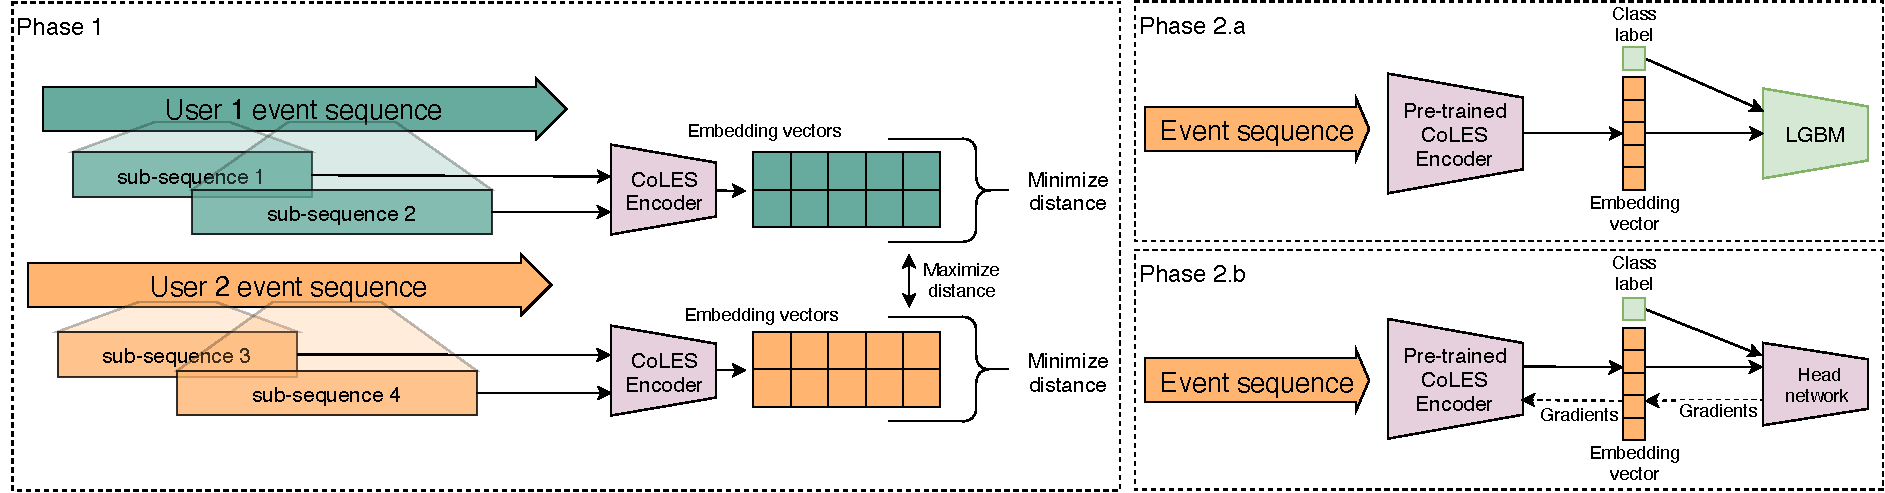
\includegraphics[width=\linewidth]{figures/CoLES.pdf}
    \caption{
        General framework.
        %
        Phase 1: Self-supervised training.
        %
        Phase 2.a Self-supervised embeddings as features for supevised model.
        %
        Phase 2.b: Pre-trained encoder fine-tuning.
    }
  \label{fig-arch}
\end{figure*}

\section{Related work} \label{sec-rel-work}

Contrastive learning has been successfully applied to constructing low-dimensional representations
(embeddings) of various objects, such as images~\citep{Chopra2005LearningAS,Schroff2015FaceNetAU},
texts~\citep{Reimers2019SentenceBERTSE}, and audio recordings~\citep{Wan2018GeneralizedEL}.
%, in a \textit{supervised} manner, where the same \textit{entity} can be represented by different \textit{samples}.
Although the aim of these studies is to identify the object based on its sample
\citep{Schroff2015FaceNetAU,Hu2014DiscriminativeDM,Wan2018GeneralizedEL}, these supervised
approaches are not applicable to our setting, since their training datasets explicitly contain
multiple independent samples per each particular object, which form positive pairs as
a critical component for learning. 

For situations when positive pairs are not available or their amount is limited, synthetic data
generation and augmentation techniques could be employed. One of the first such frameworks was
proposed by \citet{Dosovitskiy2014DiscriminativeUF}, who introduce surrogate classes by randomly
augmenting the same image. Several recent works, e.g. \citep{Bachman2019LearningRB,He2019MomentumCF,Chen2020ASF},
extended this idea by applying contrastive learning methods (see \citep{Falcon2020AFF}).
% Although augmentation techniques proposed in these studies provide good performance empirically,
% we note that no theoretical background behind different augmentation approaches has been proposed so far.
%
Contrastive Predictive Coding (CPC) is a self-supervised learning approach proposed for non-discrete
sequential data in \citep{Oord2018RepresentationLW}. The CPC employs an autoregressive predictive
model of the input sequence in order to extract meaningful latent representations, and as such
can be adapted the domain of discrete event sequences (see Section~\ref{sec-res} for comparison
with CoLES).
% CPC representations demonstrated strong performance on four distinct domains: audio, computer
% vision, natural language and reinforcement learning.

% One of the difficulties with applying a contrastive learning approach to the discrete event
% sequences is that the notion of semantic similarity as well as dissimilarity requires underlying
% domain knowledge and human labor-intensive labeling process to constrain positive and negative examples.

%In the computer vision domain, there are many other self-supervised approaches besides contrastive learning, they are nicely summarized in~\citep{Jing2020SelfsupervisedVF}. One of the common approaches to learn self-supervised representations is either traditional autoencoder~\citep{Rumelhart1986LearningIR} or variational autoencoder~\citep{Kingma2014AutoEncodingVB}. These methods are widely used for images, text and audio or aggregated event sequence data~\citep{Mancisidor2019LearningLR}. Although autoencoders have been successfully used in several domains listed above, they have not been applied to discrete event sequences, mainly due to the challenges of defining distances between the input and the output reconstructed sequences.

Several publications consider self-supervision for user behavior sequences in the recommender system
and user behavior analysis domains. CPC-like approach for self-supervised learning on user click
histories is proposed in \citep{Zhou2020ContrastiveLF}, while \citep{Ma2020DisentangledSI} use
\attn{an auxiliary self-supervised loss term}.
% \GG{For the reasons of formatting, authors do not appear in the text, and therefore, some references have now strange contexts (see examples just below). Please, find and review all "cite" contexts throughout the paper.}
% 
In~\citep{Zhou2020S3RecSL}, it was proposed to use ``Cloze'' task from BERT~\citep{Devlin2019BERTPO}
for self-supervision on purchase sequences.
% \attn{uninfromative: what is CLOZE, how it is used?}
% \GG{It is not conventional to use "[..]" as a subject that can act (proposes, adapts, ...)} 
A SimCLR-like approach for text-based tasks and tabular data was adapted in \citep{Yao2020SelfsupervisedLF}.
\revised{
In~\citep{Zhuang2019AttributedSE} authors propose an unsupervised autoregressive method
to produce embeddings of attributed sequences where a sequence of categorical tokens has additional
global attributes.
}
The aforementioned works consider sequences of ``items'', where each element is an item identifier.
We consider more complex sequences of events where an element of the sequence consists of several
categorical and numerical fields.
% Although there has been significant progress on contrastive learning, augmentation for contrastive
% learning does not have any theoretical grounding and is understudied in the domain of discrete event sequences.

There are papers dedicated to supervised learning for discrete event sequences, e.g. \citep{Wiese2009CreditCT,Tobback2019RetailCS,Babaev2019ETRNNAD,chatterjee2003modeling,sinha2014your},
but self-supervised pre-training is not used in those works.

% We briefly review its general idea. Assume that each entity $e$ is identified with a probabilistic
% distribution $P_e$ over all possible samples (e.g., in face recognition, a person is ``idenififed''
% with a distribution over all photos that can potentially be taken during their life). The idea is
% to train encoder $M$ such that samples of the same or similar entities represented in the feature
% space are closer to each other than samples of different (dissimilar) entities. Mapping $M$ defines
% a pushforward $P_M(e) := M\#P_e$ of distribution $P_e$ in the feature space $\R^d$ for each entity
% $e$. In these terms, contrastive learning tends to separate distributions $P_M(e)$ of different
% entities $e$ as much as possible.

\section{Problem formulation and overview of the CoLES method} \label{sec-method}

\subsection{Problem formulation} \label{sec:problem setting}

While the method proposed in this study could be studied in different domains, we focus on discrete
sequences of events. Assume there are some entities $e$, and the life activity of each entity~$e$ is
observed as a sequence of events $
    x_e := \{x_e(t)\}^{T_e}_{t=1}
$. Entities could be people or organizations or some other abstractions. Events $x_e(t)$ may have
any nature and structure (e.g., transactions of a client, click logs of a user), and their components
may contain numerical, categorical, and textual fields (see datasets description in Section~\ref{sec-exp}). 
% $\{x_e(t)\}^{T_e}_{t=1}$.

According to theoretical framework of contrastive learning proposed in \citep{Saunshi2019ICML}, each
entity $e$ is a latent class, which is associated with a distribution $P_e$ over its possible samples
(event sequences). However, unlike the problem setting of \cite{Saunshi2019ICML}, we have no positive
pairs, i.e. pairs of event sequences representing the same entity $e$. Instead, we have only one
sequence $x_e$ per entity~$e$. Formally, each entity $e$ is associated with a latent stochastic
process $
    \{X_e(t)\} = \{X_e(t)\}_{t\geq 1}
$, and we observe \emph{only a single} finite realisation $
    \{x_e\} = \{x_e(t)\}_{t=1}^{T_e}
$ of it. Our goal is to learn an \emph{encoder} $M$ that maps event sequences into a feature space~$\R^d$
in such a way that the obtained \emph{embedding} $
    \{x_e\} \mapsto c_e = M(\{x_e\}) \in \R^d
$ encodes the essential properties of $e$ and disregards irrelevant noise contained in the sequence.
That is, the embeddings $M(\{x'\})$ and $M(\{x''\})$ should be close to each other, if $x'$ and
$x''$ are paths generated by the same process $\{X_e(t)\}$, and further apart, if generated by distinct
processes.

The quality of representations can be examined by downstream tasks in the two ways:
\begin{enumerate}
    \item $c_e$ can be used as a feature vector for a task--specific model (see Figure~\ref{fig-arch}, Phase 2a),
    \item encoder $M$ can also be (jointly) fine-tuned~\citep{Yosinski2014HowTA} (see Figure~\ref{fig-arch}, Phase 2b).
\end{enumerate}

\subsection{Sampling of surrogate sequences as an augmentation procedure} \label{sec-pos-pairs}

When there is no sampling access to the latent processes $\{X_e(t)\}$, one could employ synthetic
augmentation strategies, which are akin to bootstrapping. Most augmentation techniques proposed
for continuous domains, such as image displacement, color jitter or random gray scale in CV, \citep{Falcon2020AFF},
are not applicable to discrete events. Thus, generating \emph{sub-sequences} from the same event
sequence $\{x_e(t)\}$, could be used as a possible augmentation.
%
The idea proposed below resembles the bootstrap method, \citep{Efron1994Bootstrap}, which, roughly,
posits that \emph{the empirical distribution} induced by the observed sample of \emph{independent}
datapoints, is a suitable proxy for the \emph{distribution of the population}.
% 
In our setting, however, the events are not independent observations, which prompts us to should
rely on different data assumptions.

The key property of event sequences that represent life activity is periodicity and repeatability
of its events (see Section~\ref{sec-period} for the empirical observations of these properties
for the considered datasets). This motivates the \emph{Random slices} sampling method applied
in CoLES, as presented in Algorithm~\ref{alg-slce-ss}. Sub-sequences $\{\tilde{x}_e\}$ are sampled
from a given sequence $\{x_e(t)\}$ as continuous segments, ``slices'', using the following three
steps.
\revised{
    First, the length of the slice is chosen uniformly from admissible values.
    Second, too short (and, optionally, too long) sub-sequences are discarded.
    Third, the starting position is uniformly chosen from all possible values.
}
The overview of the CoLES method is presented in Figure \ref{fig-arch}.
% It would seem that the mean length of obtained sub-sequences are less than the mean length
% of sequences in the dataset. However, we show in the next section that the distribution
% of sub-sequences is close to the initial distribution in some realistic assumptions.

\begin{algorithm}
    \SetAlgoLined
    \textbf{hyperparameters:}
        $m, M$: minimal and maximal possible length of a sub-sequence;
        $k$: number of samples.
    \\ %sub-sequences to be produced. \\
    \textbf{input:}
        A sequence $S = \{z_j\}_{j=0}^{T-1}$ of length $T$.
    \\
    \textbf{output:}
        $\mathcal{S}$: sub-sequences of $S$.
    \\
    \BlankLine
    \For{$i\leftarrow 1$ \KwTo $k$}{
        Generate a random integer $T_i$ uniformly from $[1, T]$;
        \\
        \uIf{$T_i\in [m, M]$}{  % burn-in and burn-out?
            Generate a random integer $s$ from $[0, T - T_i)$;
            \\
            Add the slice $
                \tilde{S}_i := \bigl\{z_{s + j}\bigr\}_{j=0}^{T_i - 1}  % S[s : s + T_i - 1]
            $ to $\mathcal{S}$;
            \\
        }
    }
    \caption{Random slices sub-sequence generation strategy}
    \label{alg-slce-ss}
\end{algorithm}


\subsection{Model training} \label{sec-training}

\textbf{Batch generation.} The following procedure creates a batch during CoLES. $N$ initial
sequences are randomly taken and $K$ sub-sequences are produced for each of one. Pairs of
sub-sequences of from same sequence are used as positive samples and pairs from different
sequences -- as negatives.
% Hence, after positive pair generation, each batch contains %$N \times K$ sub-sequences used
% as training samples. There are $NK(K-1)/2$ positive pairs and can potentially have $K^2N(N - 1)/2$
% negative pairs (not all negative pairs are considered, due to negative sampling).

%!!! REMOVED BLOCK
\begin{comment}
\begin{algorithm}
    \SetAlgoLined
    \textbf{hyperparameters:}
        $k$: number of sub-sequences to be produced.
    \\
    \textbf{input:}
        A sequence $S$ of length $l$.
    \\
    \textbf{output:}
        $S_1,...,S_k$: sub-sequences of $S$.
    \\
    \BlankLine
    Generate vector $inds$ of length $l$ with random integers from [1,k].\\
    \For{$i\leftarrow 1$ \KwTo $k$}{
        $S_i = S[inds == i]$
    }
    \caption{Disjointed sub-sequences generation strategy}
    \label{alg-disj-ss}
\end{algorithm}
\end{comment}

\revised{
In the experiment section we consider several baseline empirical strategies for the sub-sequence
generation to compare with Algorithm~\ref{alg-slce-ss}. The details of the comparison are presented
in Section~\ref{sec-ablation}.
}
% Note, that the order of events in generated sub-sequences is always preserved.

%\subsection{Contrastive learning losses} \label{sec-ml-loss}

% We consider several contrastive learning losses that showed promising performance on different
% datasets~\citep{Kaya2019DeepML} and some classical variants: contrastive~loss~\citep{Hadsell2006DimensionalityRB},
% binomial deviance loss~\citep{Yi2014DeepML}, triplet loss \citep{Hoffer2015DeepML}, histogram loss
% \citep{Ustinova2016LearningDE}, and margin loss \citep{Manmatha2017SamplingMI}. Among them,
% contrastive loss showed best performance in experiments (see Appendix~\ref{app-sec-design}).
% $
%     \mathcal{L}
%         = (1 - Y) \frac12 (D_W^i)^2
%         + Y \frac12\max\{0, m - D_W^i \}^2
% $
\textbf{Contrastive loss} We consider a classical variant of the contrastive loss, proposed in
\citep{Hadsell2006DimensionalityRB}, which minimizes the objective
\begin{equation*}
    \mathcal{L}_{u v}(M)
        = Y_{u v} \frac12 d_M(u, v)^2
        + (1 - Y_{u v}) \frac12\max\{0, \rho - d_M(u, v) \}^2
    \,,
\end{equation*}
with respect to $
    M \colon \mathcal{X} \to \mathbb{R}^n
$, where $
    d_M(u, v) = d(c_u, c_v)
$ is the distance between embeddings of the pair $(u, v)$, $
    c_* = M(\{\tilde{x}_*(\tau)\})
$, $Y_{u v}$ is a binary variable
identifying whether the pair $(u, v)$ is positive, and $\rho$ is the soft minimal margin between
dissimilar objects. The second term encourages separation of the embeddings in negative
pairs and prevents \emph{mode collapse} in $M$, when the entities are mapped to the same
point in the embedding space. $d(a, b)$ is the Euclidean distance, $
    d(a, b)
        = \sqrt{
            \sum_k (a_k - b_k)^2
        }
$, as proposed in~\citep{Hadsell2006DimensionalityRB}.
%  ATTN (ivannz) this could use some survey reference from
% https://lilianweng.github.io/lil-log/2021/05/31/contrastive-representation-learning.html
The sequences $\{\tilde{x}_u(\tau)\}$ and $\{\tilde{x}_v(\tau)\}$ of a pair with $Y_{u v} = 1$
are obtained through random slice generation (Algorithm~\ref{alg-slce-ss}) from the \emph{same}
observation $\{x_e(t)\}$, while in pairs with $Y_{u v} = 0$ the sequences are sampled from
$\{x_e(t)\}$ and $\{x_g(t)\}$, respectively, for $e \neq g$.

\revised{
In the experiment section we compare the basic variant of the contrastive loss
with alternative variants. The results of the comparison is presented in Section~\ref{sec-ablation}.
}
%(see Appendix~\ref{app-sec-pair-dist}).

\textbf{Negative sampling.} One challenge in contrastive learning approach is that positive pairs
are overwhelmed by potential negative pairs. Furthermore, some of negative pairs are distant enough,
to not provide any valuable feedback through $\mathcal{L}$ to $M$ during training, \citep{SimoSerra2015DiscriminativeLO,Schroff2015FaceNetAU}. We compare the common negative sampling
methods in Section~\ref{sec-res}. Since certain negative sampling approaches are distance-aware and
to make the overall distance computation less inefficient we restrict the encoder $M$ to the class
of maps that output vectors on a unit hyper-sphere in $\R^d$. Therefore the pairwise distance $
    d_M(u, v)^2
$ is just $2 - 2 c_u^\top c_v$, which only requires pairwise dot products between embeddings $
    c_v = M(\{\tilde{x}_u(t)\})
$.

\subsection{Encoder architecture} \label{sec-enc-arch}

Embedding a sequence of events into a vector of fixed size requires encoding individual events
followed by aggregating the entire sequence. The composite encoder model $M$ in CoLES is of
the form $
    M(\{x_t\})
        := \phi_{\mathrm{seq}}(\{\phi_{\mathrm{evt}}(x_t)\})
$, where $\phi_{\mathrm{evt}}$ and $\phi_{\mathrm{seq}}$ are event-level and sequence-level networks,
respectively, trained in an end-to-end manner.

\textbf{The event encoder} $\phi_{\mathrm{evt}}$ takes a set of attributes of each event $x_t$
and outputs its intermediate representation in $\R^d$: $z_t = \phi_{\mathrm{evt}}(x_t)$. This
encoder consists of several embedding layers and batch normalization layers. Each categorical
attribute is encoded by \attn{its corresponding embedding layer}. Batch normalization is applied
to numerical attributes of events. Outputs of all embedding and batch normalization layers are
concatenated to produce $z_t$.

\textbf{The sequence encoder} $\phi_{\mathrm{seq}}$ takes the intermediate representations of
the events $ z_{1:T} = z_1, z_2, \cdots z_T $ and outputs the representation $c_t$ of their
sequence up to the time $t$: $c_t = \phi_{\mathrm{seq}}(z_{1:t})$. The last output $c_T$ is used
as the embedding of the whole event sequence.
\revised{
In our experiments, we use GRU, \citep{Cho2014OnTP}, recurrent network which demonstrats
robust performance on the sequential data, \citep{Babaev2019ETRNNAD}. In this case, $\phi_{\mathrm{seq}}$
is computed with the recurrence $c_{t+1} = \mathrm{GRU}(z_{t+1}, c_t)$ starting from $c_0 = 0$.
We note, that other architecture choice are possible, including LSTM and transformers, \citep{Hochreiter1997LongSM,Vaswani2017AttentionIA} (see Section~\ref{sec-ablation}).
}

\medskip
To summarise, CoLES consists of three major ingredients: the event sequence encoder, the positive
and negative pair generation strategy, and the loss function for contrastive learning.

% In the next section, we describe our experiments of the comparison of the proposed method
%  with several strong baselines on several public datasets.

\section{Experiments} \label{sec-exp}

\subsubsection{Datasets}

We compare our method with existing baselines on several publicly available datasets of
event sequences from various data science competitions. We chose datasets with sufficient
amounts of discrete events per user.

\textbf{Age group prediction competition}%
\footnote{
    \url{https://ods.ai/competitions/sberbank-sirius-lesson}
}
The dataset of 44M an\-onymized credit card transactions representing 50K individuals
was used to predict the age group of a person.
\attn{The label is known for 30K records, other 20K are unlabelled.}
The group ratio is balanced in the dataset. Each transaction includes the date, type,
and amount being charged.

% \textbf{Gender prediction competition}%
% \footnote{
%     \url{https://www.kaggle.com/c/python-and-analyze-data-final-project/}
% }
% The dataset of 6.8M anonymized card transactions representing 15K clients was used to
% predict gender. Each transaction is characterized by date, type, amount and Merchant Category Code.

\textbf{Churn prediction competition}%
\footnote{
    \url{https://boosters.pro/championship/rosbank1/}
}
The dataset of 1M an\-onymiz\-ed card transactions representing 10K clients was used to
predict churn probability. Each transaction is characterized by date, type, amount and
Merchant Category Code. 5K clients have labels, 5.2K clients are unlabelled labels.
Target is binary, almost balanced with proportions $55:45$.

\textbf{Assessment prediction competition}%
\footnote{
    \url{https://www.kaggle.com/c/data-science-bowl-2019}
}
The task is to predict the in-game assessment results based on the history of children's
gameplay data. Target is one of four grades, with shares $0.50$, $0.24$, $0.14$, $0.12$.
The dataset consists of 12M gameplay events combined in 330K gameplays representing 18K
children. 17.7K gameplays are labeled, the remaining 312K gameplays are not labeled.
Each gameplay event is characterized by a timestamp, an event code, an incremental counter
of events within a game session, time since the start of the game session, etc.

\textbf{Retail purchase history age group prediction}%
\footnote{
    \url{https://ods.ai/competitions/x5-retailhero-uplift-modeling}
}
The task is to predict the age group of a client based on their retail purchase history.
The group ratio is balanced in the dataset. Only labeled data is used. The dataset consists
of 45.8M retail purchases representing 400K clients. Each purchase is characterized by
time, product level, segment, amount, value, loyalty program points received.

\textbf{Scoring competition}%
\footnote{
     \url{https://boosters.pro/championship/alfabattle2/overview}
}
The dataset of 443M anonymized credit card transactions representing 1.47M persons was
used to predict the probability of credit product default. The label is known for 0.96M
persons, other 0.51M are unlabelled. The default rate is 2.76\% in the dataset. Each
transaction includes the set of date features, set of type features, and amount being
charged.

% As we can see in Figure~\ref{fig-seq-len} (Appendix~\ref{app-sec-data}), these datasets satisfy the power law assumption for the sequence length distribution of Theorem~\ref{thm:distribution}. Also, as shown in Figure~\ref{fig-subseq-kl} (Appendix~\ref{app-sec-data}) the datasets satisfy the periodicity and repeatability assumption.

\subsubsection{Repeatability and periodicity of the datasets} \label{sec-period}

\begin{figure*}
  \centering
  \begin{subfigure}{0.25\linewidth}
    \caption{Age group}
    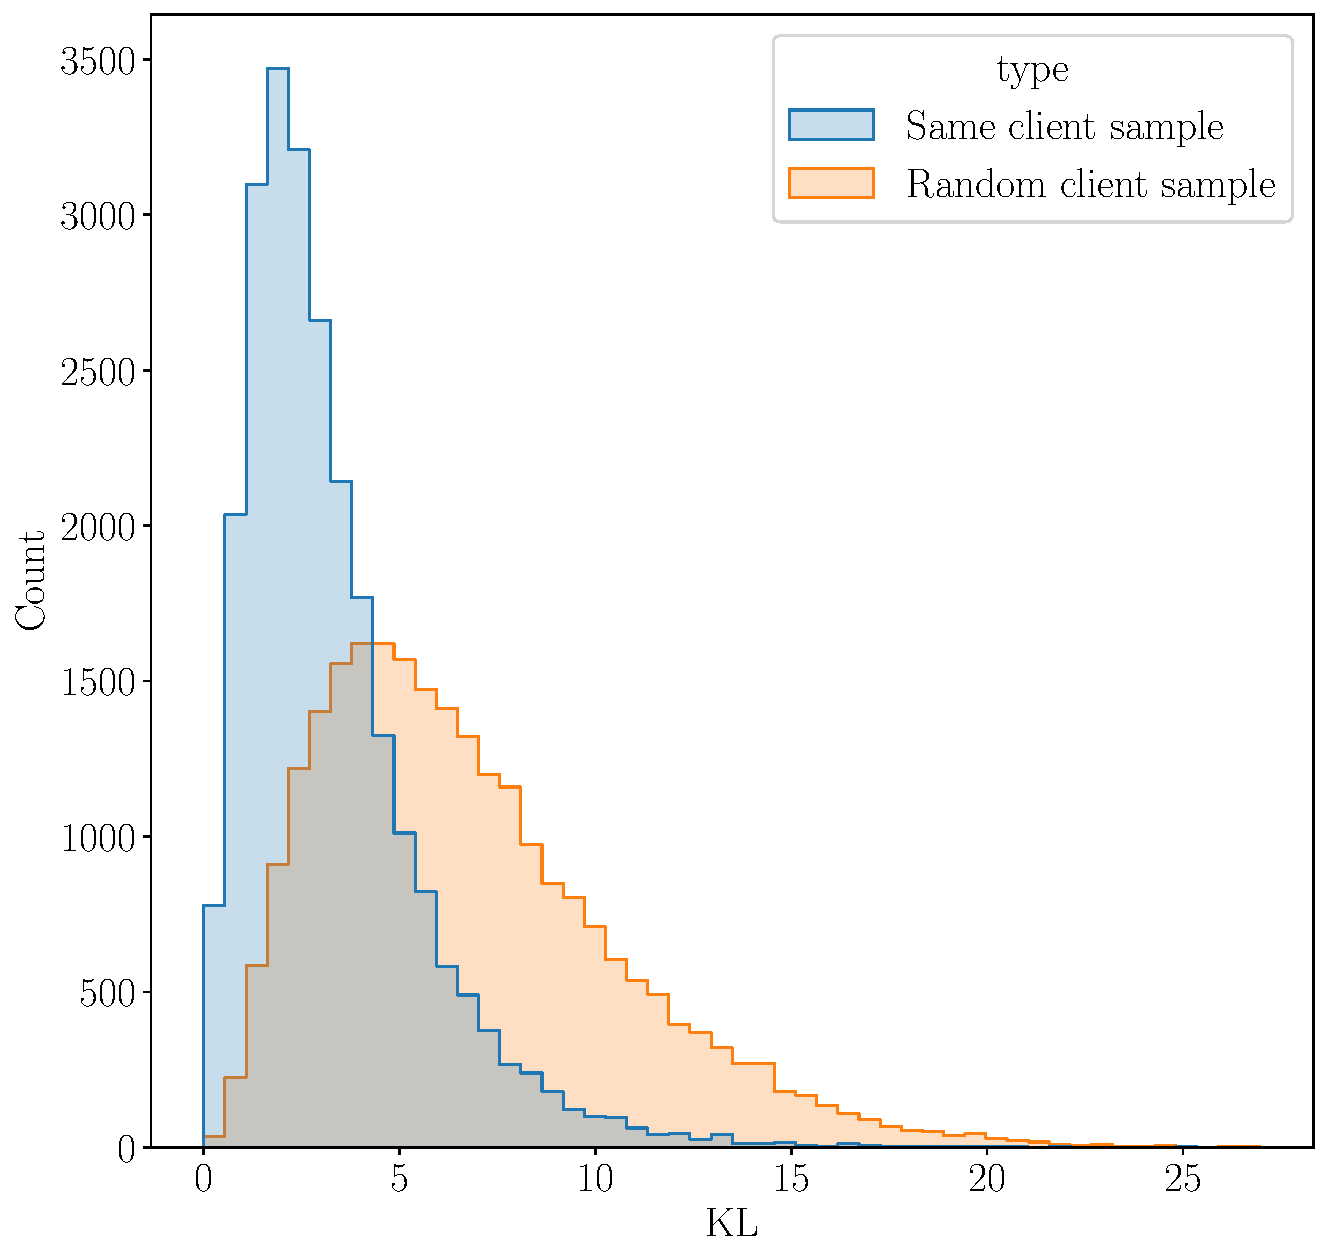
\includegraphics[width=\linewidth]{figures/kl_dis_age_group.pdf}
  \end{subfigure}%
  %\begin{subfigure}{0.5\linewidth}
  %  \caption{Churn}
  %  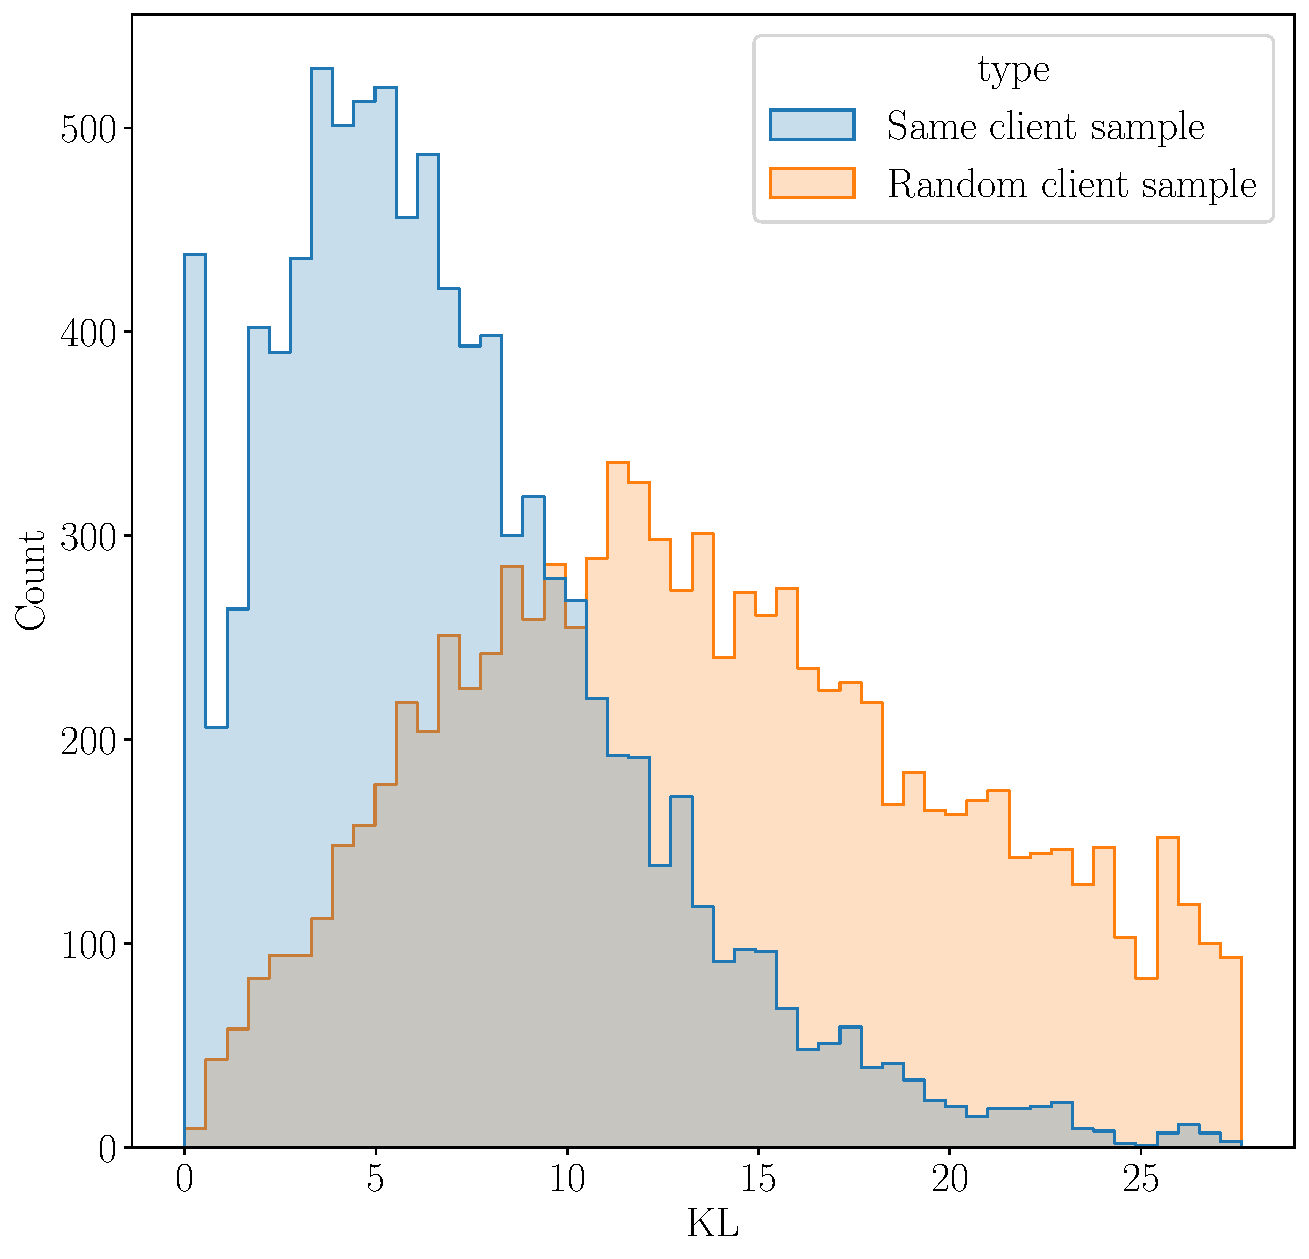
\includegraphics[width=\linewidth]{figures/kl_dis_churn.pdf}
  %\end{subfigure}
  \begin{subfigure}{0.25\linewidth}
    \caption{Assessment}
    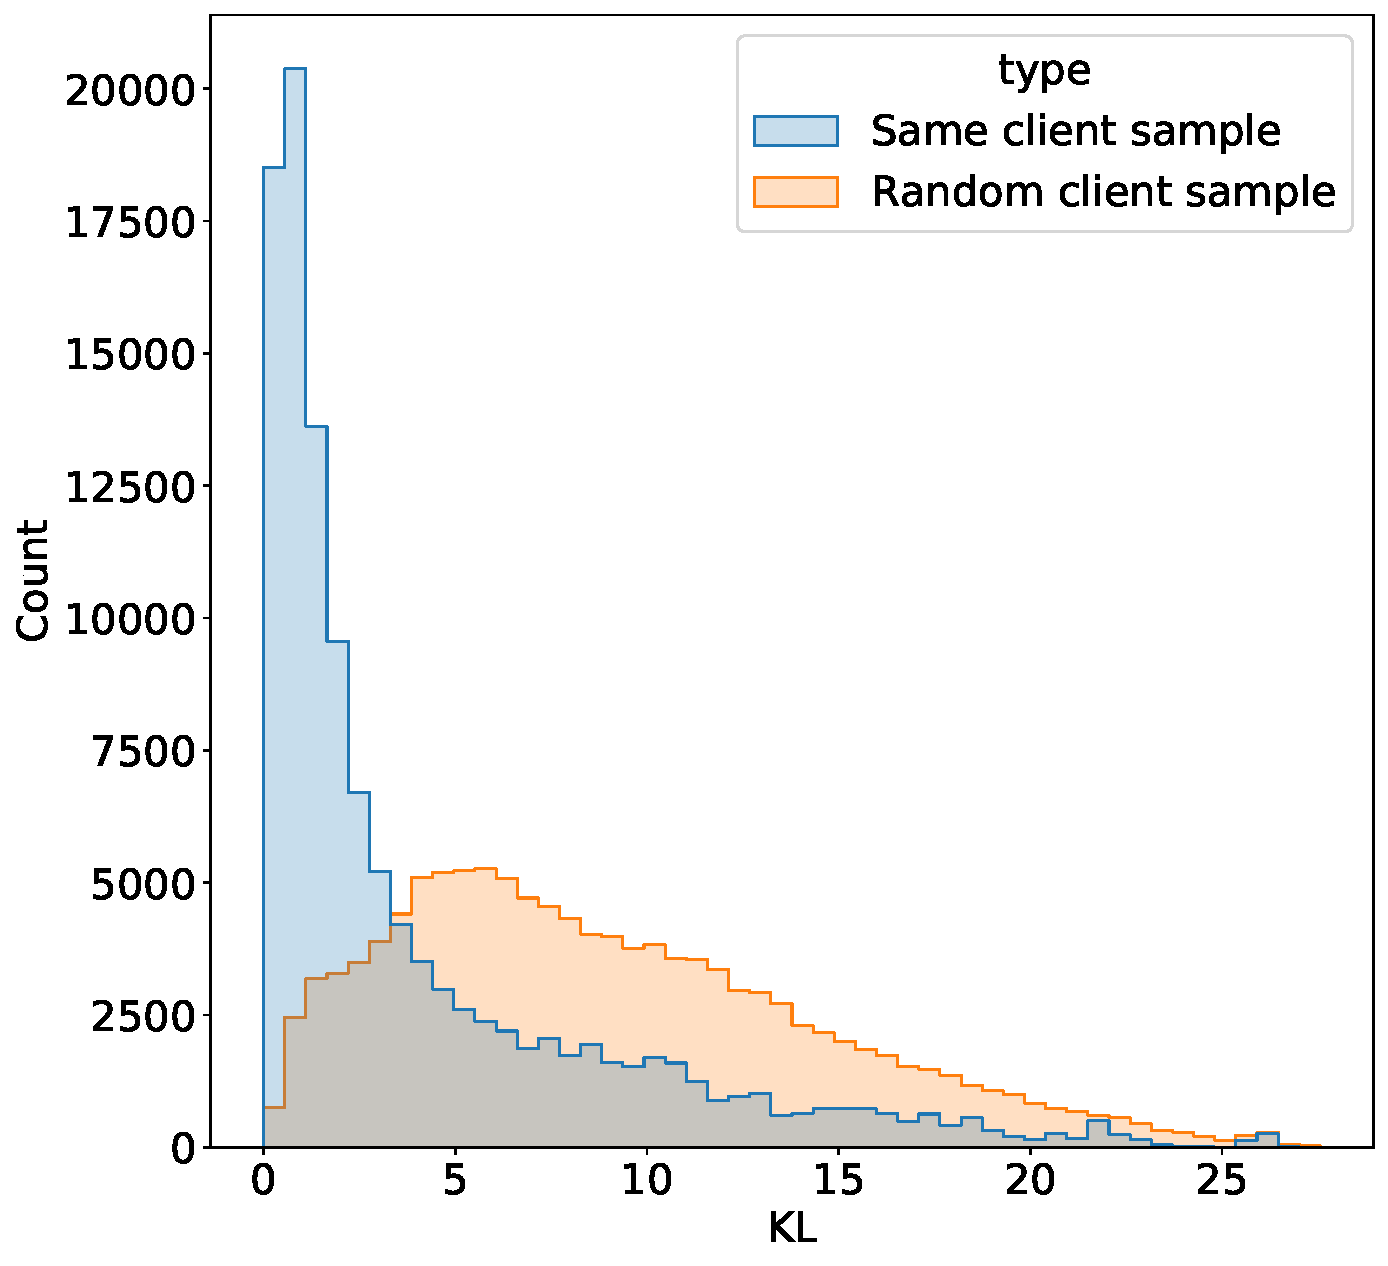
\includegraphics[width=\linewidth]{figures/kl_dis_assessment.pdf}
  \end{subfigure}%
  \begin{subfigure}{0.25\linewidth}
    \caption{Retail}
    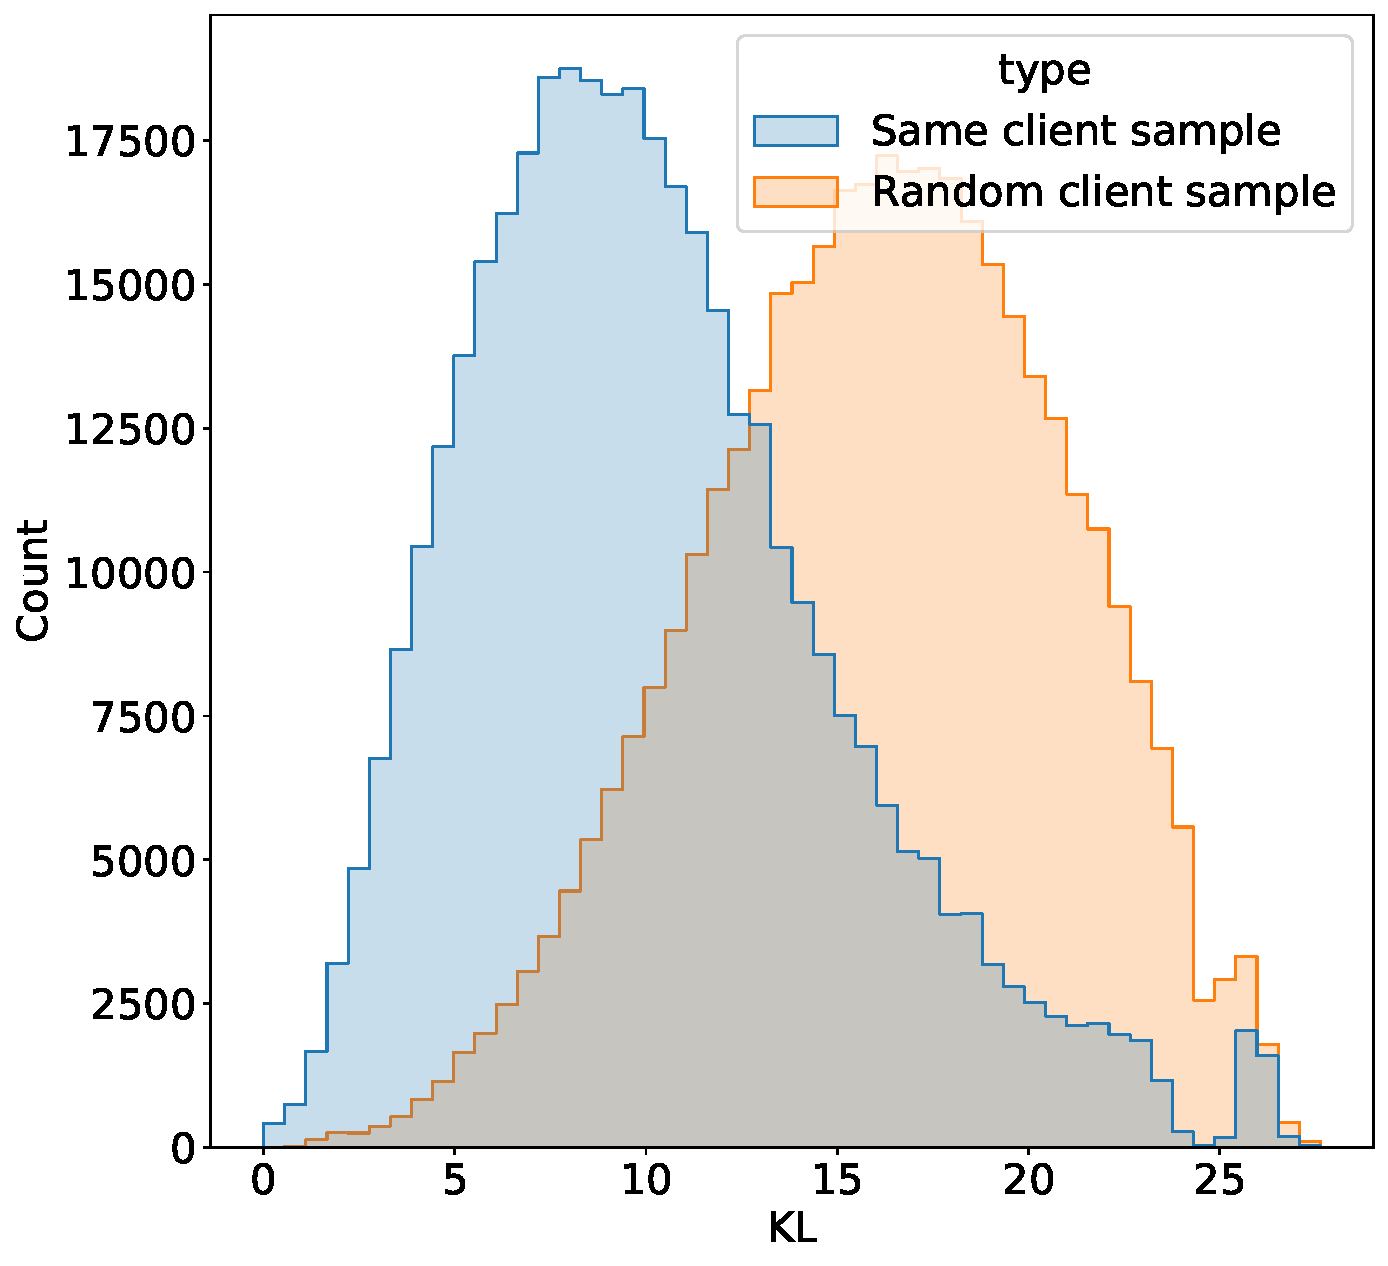
\includegraphics[width=\linewidth]{figures/kl_dis_retail.pdf}
  \end{subfigure}%
  \begin{subfigure}{0.25\linewidth}
    \caption{Texts}
    \centerline{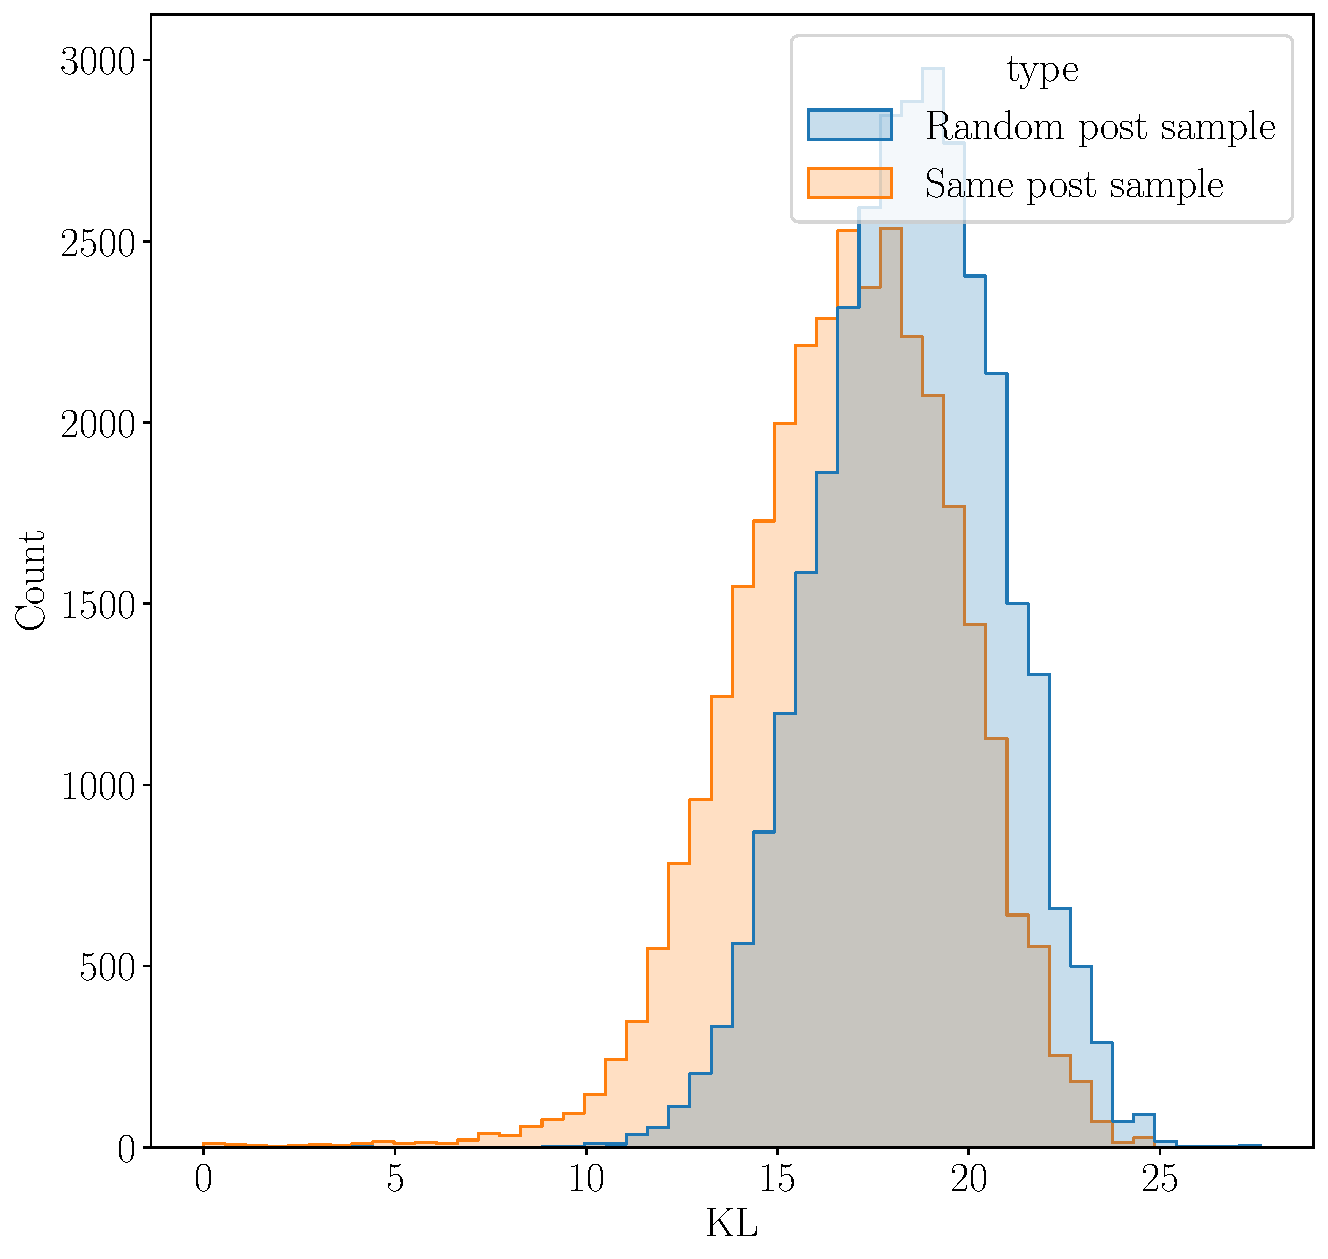
\includegraphics[width=\linewidth]{figures/kl_dis_text.pdf}}
    \label{fig-subseq-kl-texts}
  \end{subfigure}
  \caption{
    Periodicity and repeatbility of the data. KL-divergence between event types
    of two random sub-sequences from the same sequence is compared with KL-divergence
    between sub-sequences of different sequences. Additional plot (\ref{fig-subseq-kl-texts})
    is provided as an example for data without any repeatable structure.
  }
  \label{fig-subseq-kl}
\end{figure*}

To check that considered datasets follow our repeatability and periodicity assumption
made in Section~\ref{sec-pos-pairs}
%and used for theoretical analysis in Section~\ref{sec-theory}
we performed the following experiments. We measure the KL-divergence between two kinds
of samples:
(1) between random slices of the same sequence, generated using a modified version of
Algorithm~\ref{alg-slce-ss} where overlapping events are dropped, and
(2) between random sub-samples taken from different sequences. The results are shown in
Figure~\ref{fig-subseq-kl}, which shows that the KL-divergence between sub-sequences of
the same sequence of events is relatively small compared to the typical KL-divergence between
sub-samples of different sequences of events. This observation supports our repeatability
and periodicity assumption.
Also note that additional plot (\ref{fig-subseq-kl-texts}) is provided as an example for
data without any repeatable structure.

\subsubsection{Dataset split}

For each dataset, we set apart 10\% persons from the labeled part of the data as the \textit{test set} that we used for evaluation of different models. The rest 90\% of labeled data and unlabeled data constitute our \textit{training set} used for learning. For all methods, a random search on 5-fold cross-validation over the training set is used for hyper-parameter selection. The hyper-parameters with the best out-of-fold performance are then chosen.
For the learning of semi-supervised/self-supervised techniques (including CoLES), we used all transactions of training sets including unlabeled data. The unlabelled parts of the datasets were ignored while training supervised models.

\subsubsection{Training performance}

Neural network training was performed on a single Tesla P-100 GPU card. For the training part of CoLES, the single training batch is processed in 142 milliseconds. For example, in the age group prediction dataset the single training batch contains 64 unique persons with 5 sub-sequences per person, i.e. 320 training sub-sequences in total, the mean number of transactions in a sub-sequence is 90, hence, each batch contains about 28800 transactions.

\subsubsection{Hyperparameters}

Unless we explicitly specify, we use contrastive loss and random slices pair generation strategy for CoLES in our experiments (see Section~\ref{sec-res} for motivation). The final set of hyper-parameters used for CoLES is shown in the Table \ref{tab-hyper}.

\begin{table}
\centering
\caption{Hyper-parameters for CoLES training}
\begin{tabularx}{\linewidth}{Xcccc}
\toprule
\textbf{Dataset} & \textbf{Age} & \textbf{Churn} & \textbf{Assess} & \textbf{Retail} \\
\midrule
\textbf{Embedding size} & 800 & 1024 & 100 & 800 \\
\textbf{Learning rate} & 0.001 & 0.004 & 0.002 & 0.002 \\
\textbf{N samples in batch} & 64 & 128 & 256 & 256 \\
\textbf{N epochs} & 150 & 60 & 100 & 30 \\
\textbf{Min sequence length} & 25 & 15 & 100 & 30 \\
\textbf{Max sequence length} & 200 & 150 & 500 & 180 \\
\textbf{Encoder} & GRU & LSTM & GRU & GRU \\
\bottomrule
\end{tabularx}
\small{For all methods, a random search on 5-fold cross-validation over the train set is used for hyper-parameter selection. The number of sub-sequences generated for each sequence was always 5 for each dataset.}
\label{tab-hyper}
\end{table}

\subsection{Baselines} \label{sec-baselines}

%We compare our CoLES method with the following baselines.

\subsubsection{LightGBM}

We consider the Gradient Boosting Machine (GBM)~\citep{Friedman2001GreedyFA} as the method to create a model for the downstream task (see Figure~\ref{fig-arch}, Phase 2a). GBM can be considered as a strong baseline in cases of tabular data with heterogeneous features.
% In particular, GBM-based approaches achieve state-of-the-art results in a variety of practical tasks including web searches, weather forecasting, fraud detection, and many others
~\citep{Wu2009AdaptingBF, Vorobev2019LearningTS, Zhang2015AGB, Niu2019ACS}. We used LightGBM~\citep{Ke2017LightGBMAH} implementation of the GBM algorithm.

GBM based model requires its input to be a flat vector of the fixed length. In our experiments we consider the following types of the input: (1) the vector of of hand-crafted aggregate features produced from the raw transactional data, (2) the embedding of the sequence of transactions, produced by the encoder network (see Section~\ref{sec-enc-arch}). The encoder model is trained in the self-supervised way either with CoLES or one of the alternative methods, described in the Section~\ref{sec-ss-base}.

\subsubsection{Hand-crafted features} \label{sec-hand-features}

We use the following approach to produce hand-crafted features. All attributes of each transaction are either numerical (e. g. amount) or categorical (e.g. merchant category (MCC code), transaction type, etc.).
For the numerical type of attribute we apply aggregation functions, such as 'sum', 'mean', 'std', 'min', 'max', over all transactions per user. For example, if we apply 'sum' for the numerical field 'amount' we obtain a feature 'sum of all transaction amounts per user'.
For the categorical type of attribute we apply aggregation functions in a slightly different way. For each unique value of categorical attribute we apply aggregation functions, such as 'count', 'mean', 'std' over all transactions per user's numerical attribute. For example, if we apply 'mean' for the numerical attribute 'amount' grouped by categorical attribute 'MCC code' we obtain one feature 'mean amount of all transactions for the specific MCC code per user.
% For example, for age prediction task we have one categorical attribute (small group) with 200 unique values, combining it with amount we can produce $200 * 3$ features ('group0 x amount x count',  'group1 x amount x count', ..., 'group199 x amount x count', 'group0 x amount x mean', ...). In total we use approx 605 features for this task.

\subsubsection{Self-supervised baselines} \label{sec-ss-base}

We compared CoLES method against major existing approaches to create self-supervised embeddings, which can be applied to the event sequence data.

\textbf{NSP.} We consider a simple baseline inspired by the \textit{next sentence prediction} task used in BERT~\citep{Devlin2019BERTPO}. Specifically, we generate two sub-sequences A and B, in a way that 50\% of the time B is the sub-sequence from the same sequence as A and follows it (positive pair), and 50\% of the time it is a random sub-sequence taken from another sequence (negative pair).

\textbf{SOP.} Another simple baseline is the same as \textit{sequence order prediction} task from ALBERT~\citep{Lan2020ALBERTAL}. It uses two consecutive sub-sequences as a positive pair, and two consecutive sub-sequences with swapped order as a negative pair.

\textbf{RTD.} We also adapt the \textit{replaced token detection} approach from ELECTRA~\citep{Clark2020ELECTRAPT} for event sequences as a baseline for our research. We replaced 15\% of events from the sequence with random events, taken from other sequences and train a model to predict whether an event is replaced or not.

\textbf{CPC.} As the last self-supervised baseline, we selected Contrastive Predictive Coding (CPC)~\citep{Oord2018RepresentationLW}, a self-supervised learning method that produced an excellent performance on sequential data of such traditional domains as audio, computer vision, reinforcement learning and recommender systems~\citep{Zhou2020ContrastiveLF}.
% We adapted the CPC method to the discrete event sequences by making the model task to distinguish true future events from other types of events by using a series of previous events as an input.

\subsection{Results} \label{sec-res}

\begin{table}
\centering
\caption{Comparison of batch generation strategies}
\begin{tabularx}{\linewidth}{Xcccc}
\toprule
\makecell{\textbf{Sample} \\ \textbf{method}} &
\makecell{\textbf{Age} \\ \small{Accuracy}} &
\makecell{\textbf{Churn} \\ \small{AUROC}} &
\makecell{\textbf{Assess} \\ \small{Accuracy}} &
\makecell{\textbf{Retail} \\ \small{Accuracy}} \\
\midrule
\textbf{Random samples} & 0.613 & 0.820 & 0.563 & 0.523 \\
\textbf{Random disjoint samples} & 0.619 & 0.819 & 0.563 & 0.505 \\
\textbf{Random slices} & \textbf{0.639} & \textbf{0.823} & \textbf{0.618} & \textbf{0.542} \\
\bottomrule
\end{tabularx} \\
\small{5-fold cross-validation metric is shown}
\label{tab-pair-gen}
\end{table}

\subsubsection{Design choices observations} \label{sec-ablation}

To evaluate the proposed method of sub-sequence generation (see Section~\ref{sec-pos-pairs}) we compared it with two alternative strategies: \revised{(1) The random sampling without replacement strategy and (2) random disjoint samples strategy. The random disjoint samples strategy produces sub-sequences by the random splitting of the initial sequence to several connected segments without intersection between them.
To generate k sub-sequences, the following procedure should be repeated k times: take a random number of elements from the sequence \textit{without replacement}. The motivation is that intersections between sub-sequences may possibly lead to overfitting since exact sub-sequences of events are the same and may be "remembered" without learning a deeper level of similarities.} Also, note that the random samples strategy is similar to the augmentation strategy proposed by \cite{Yao2020SelfsupervisedLF}, and the random disjoint samples strategy is similar to sub-sequence generation proposed by \cite{Ma2020DisentangledSI}.

The results of the comparison are presented in Table~\ref{tab-pair-gen}. The proposed random slices sub-sequence generation strategy significantly outperforms alternative strategies.
%, what confirm theoretical results (see Section \ref{sec-theory}).

\revised{We evaluated several contrastive learning loss functions that showed promising performance on different datasets~\citep{Kaya2019DeepML} and some classical variants, namely: contrastive~loss~\citep{Hadsell2006DimensionalityRB}, binomial deviance loss~\citep{Yi2014DeepML}, triplet loss \citep{Hoffer2015DeepML}, histogram~loss~\citep{Ustinova2016LearningDE}, and margin~loss~\citep{Manmatha2017SamplingMI}. The results of comparison are shown in the Table~\ref{tab-loss-type}. 
It is interesting to observe that even contrastive loss that can be considered as the basic variant of contrastive learning loss allows to get strong results on the downstream tasks. Our hypothesis is that an increase in the model performance on contrastive learning task does not always lead to an increase in performance on downstream tasks.}

We also compared popular negative sampling strategies (distance-weighted sampling~\citep{Manmatha2017SamplingMI}, and hard-negative mining~\citep{Schroff2015FaceNetAU}) with random negative sampling strategy.
The results are shown in the Table \ref{tab-neg-sampl}.
We found that hard negative mining leads to a significant increase in quality on downstream tasks in comparison to random negative sampling.

\revised{Yet another possible design choice of the method is the encoder architecture. We compared several popular options for the sequence encoder: GRU~\citep{Cho2014OnTP}, LSTM~\citep{Hochreiter1997LongSM} and Transformer~\citep{Vaswani2017AttentionIA}. As shown in Table~\ref{tab-enc-type}, the choice of encoder architecture does not significantly affect the performance of the proposed method.}

\begin{table}
\centering
\caption{Comparison of encoder types}
\begin{tabular}{lcccc}

\toprule
\textbf{Dataset} &
\makecell{\textbf{Age group} \\ \small{Accuracy}} &
\makecell{\textbf{Churn} \\ \small{AUROC}} &
\makecell{\textbf{Assess} \\ \small{Accuracy}} &
\makecell{\textbf{Retail} \\ \small{Accuracy}} \\
\midrule

\textbf{LSTM} & 0.621 & \textbf{0.823} & \textbf{0.620} & 0.535 \\
\textbf{GRU} & \textbf{0.638} & 0.812 & 0.618 & \textbf{0.542} \\
\textbf{Transformer} & 0.622 & 0.780 & 0.542 & 0.499 \\

\bottomrule
\end{tabular} \\
\small{5-fold cross-validation metric is shown}
\label{tab-enc-type}
\end{table}

\begin{table}
\centering
\caption{Comparison of contrastive learning losses}
\begin{tabularx}{\linewidth}{Xcccc}
\toprule
\textbf{Dataset} &
\makecell{\textbf{Age group} \\ \small{Accuracy}} &
\makecell{\textbf{Churn} \\ \small{AUROC}} &
\makecell{\textbf{Assess} \\ \small{Accuracy}} &
\makecell{\textbf{Retail} \\ \small{Accuracy}} \\
\midrule

\textbf{Contrastive} \small{margin=0.5} & \textbf{0.639} & \textbf{0.823} & \textbf{0.618} & \textbf{0.542} \\
\textbf{Binomial deviance} & 0.621 & 0.769 & 0.589 & 0.535 \\
\textbf{Histogram} & 0.632 & 0.815 & 0.615 & 0.533 \\
\textbf{Margin} & 0.638 & \textbf{0.823} & 0.612 & 0.541 \\
\textbf{Triplet} & 0.636 & 0.781 & 0.600 & 0.541 \\

\bottomrule
\end{tabularx} \\
\small{5-fold cross-validation metric is shown}
\label{tab-loss-type}
\end{table}

\begin{table}
\centering
\caption{Comparison of negative sampling strategies}
\begin{tabularx}{\linewidth}{Xcccc}
\toprule
\textbf{Dataset} &
\makecell{\textbf{Age group} \\ \small{Accuracy}} &
\makecell{\textbf{Churn} \\ \small{AUROC}} &
\makecell{\textbf{Assessment} \\ \small{Accuracy}} &
\makecell{\textbf{Retail} \\ \small{Accuracy}} \\
\midrule

\textbf{Hard negative mining} & \textbf{0.639} & \textbf{0.823} & \textbf{0.618} & \textbf{0.542} \\
\textbf{Random negative sampling} & $0.626$ & $0.815$ & $0.593$ & $0.530$ \\
\textbf{Distance-weighted sampling} & $0.629$ & $0.821$ & $0.603$ & $0.536$ \\

\bottomrule
\end{tabularx} \\
\small{5-fold cross-validation metric is shown}
\label{tab-neg-sampl}
\end{table}

\revised{Figure \ref{fig-emb-dim} shows that the performance quality on the downstream task increases with the dimensionality of an embedding. After the best quality is achieved, a further increase in the dimensionality of an embedding dramatically reduces quality.
These results can be interpreted as the bias-variance trade-off. When the embedding dimensionality is too small, too much information can be discarded (high bias). On the other hand, when embedding dimensionality is too large, too much noise is added (high variance).
Note, that increasing the embedding size will also linearly increase the training time and the volume of consumed memory on the GPU.}

\begin{figure*}
  \centering
  \caption{Embedding dimensionality vs. quality}
  \begin{subfigure}{0.25\linewidth}
    \caption{Age group}
    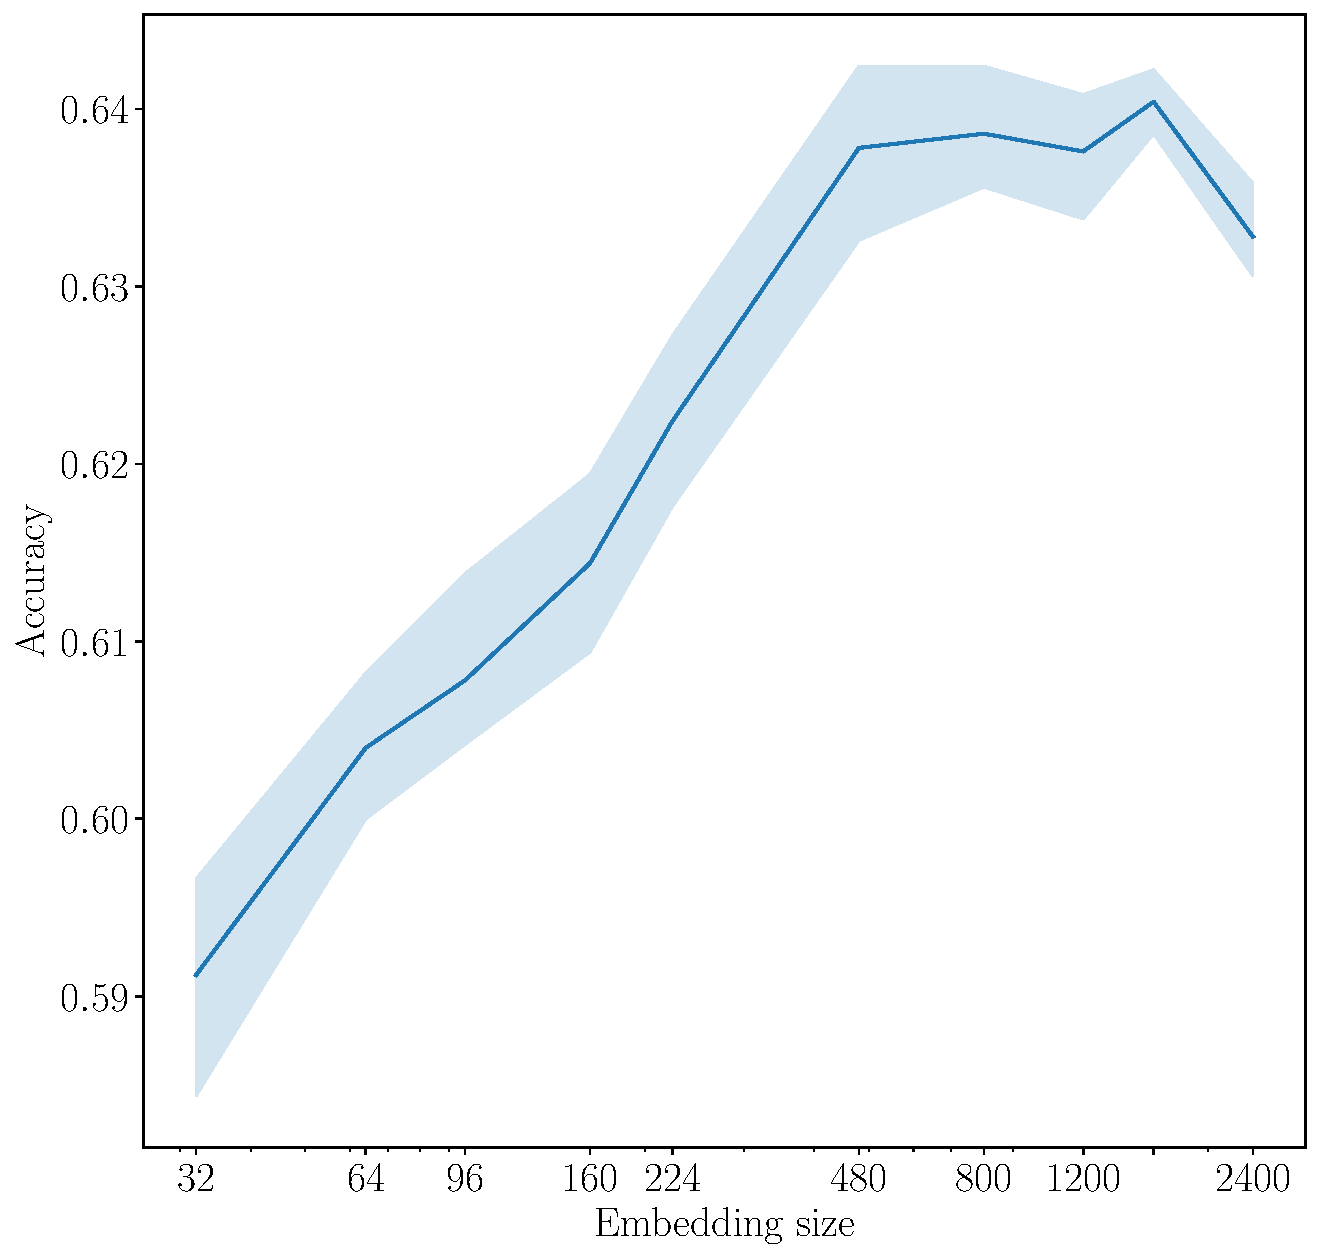
\includegraphics[width=\linewidth]{figures/hidden_size_age_pred.pdf}
  \end{subfigure}%
  \begin{subfigure}{0.25\linewidth}
    \caption{Churn}
    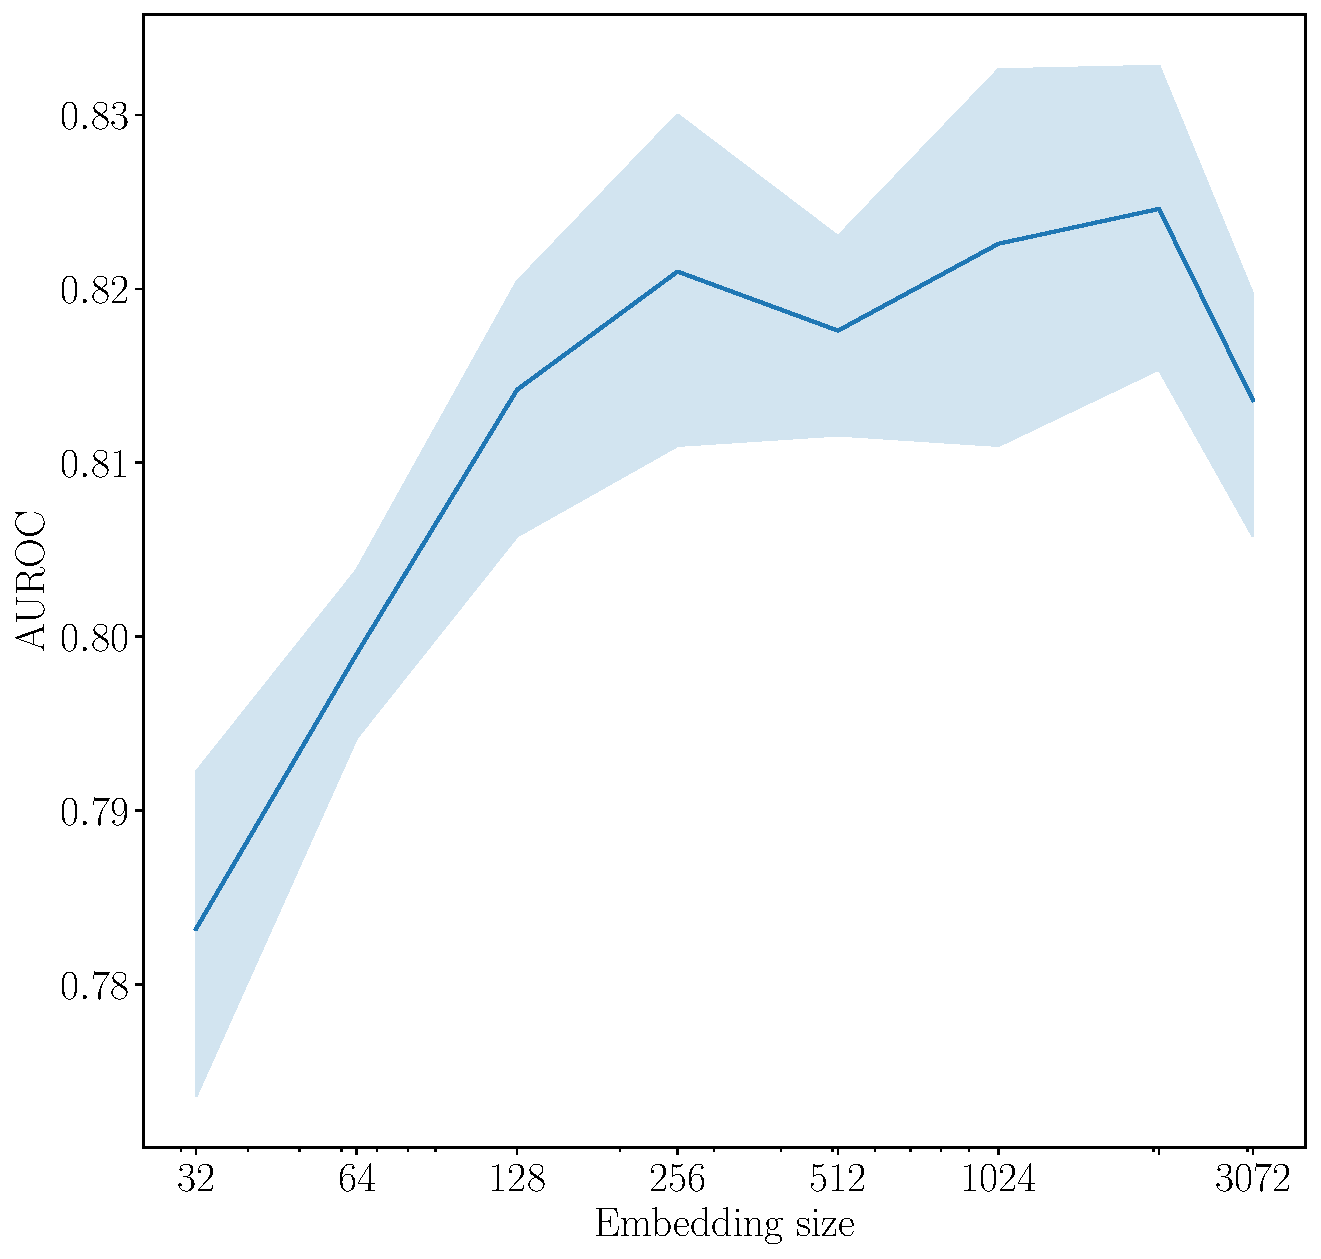
\includegraphics[width=\linewidth]{figures/hidden_size_rosbank.pdf}
  \end{subfigure}%
  \begin{subfigure}{0.25\linewidth}
    \caption{Assessment}
    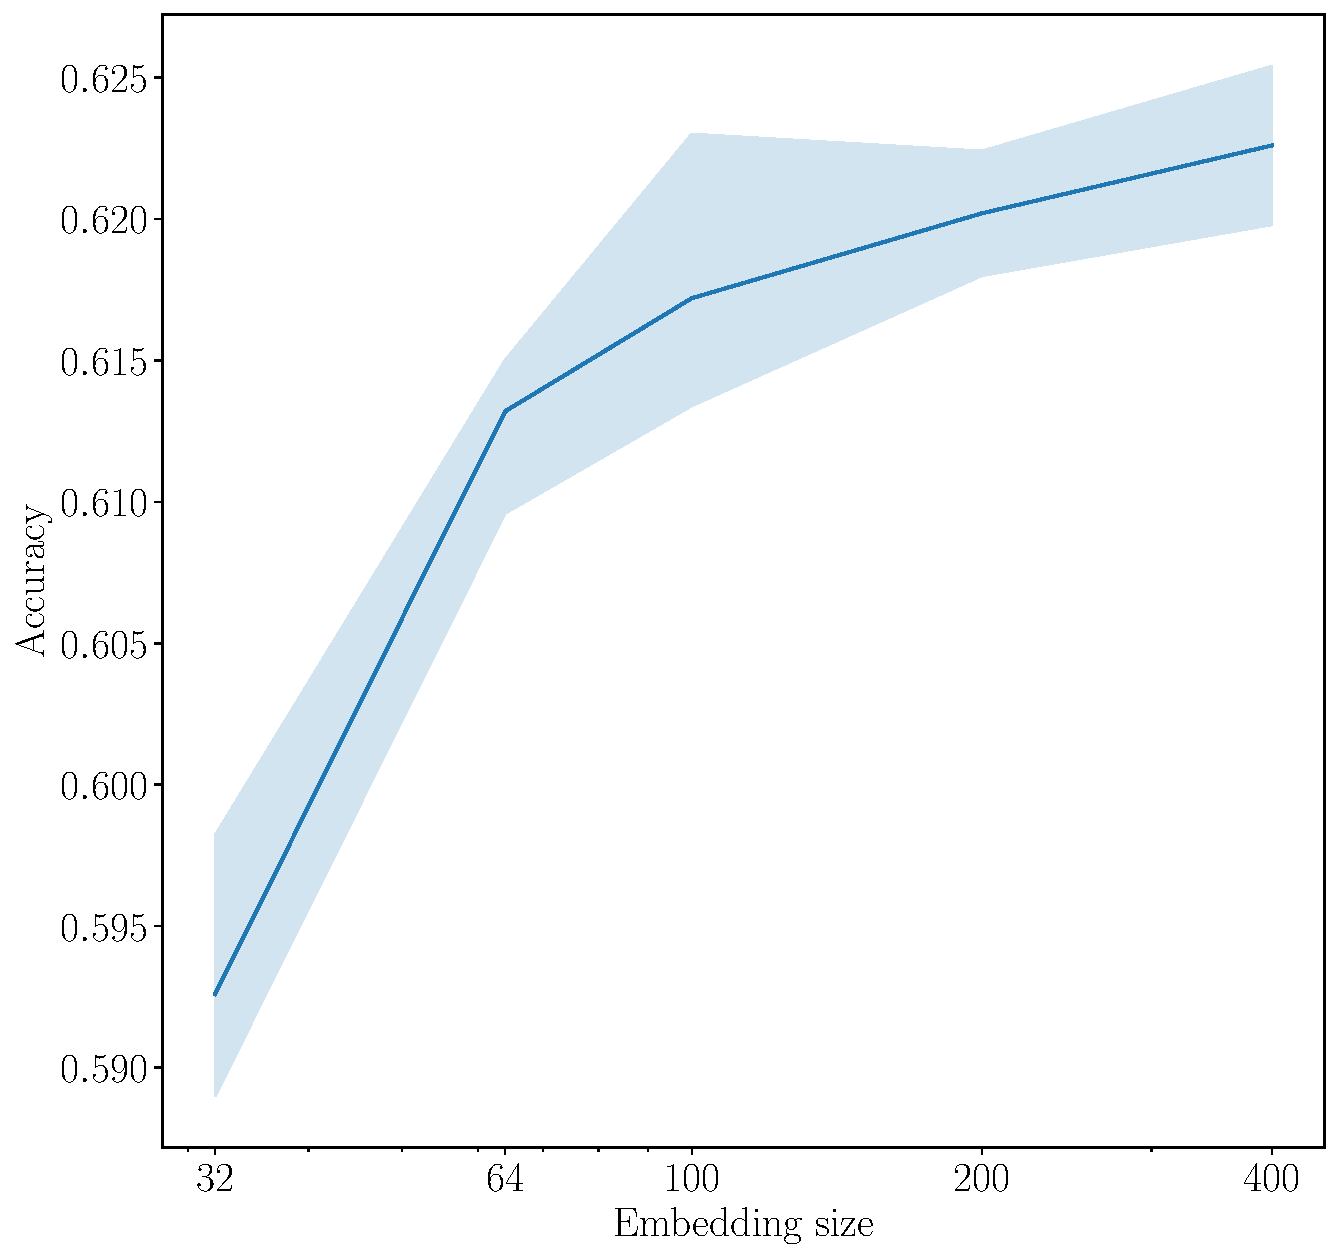
\includegraphics[width=\linewidth]{figures/hidden_size_bowl2019.pdf}
  \end{subfigure}%
  \begin{subfigure}{0.25\linewidth}
    \caption{Retail}
    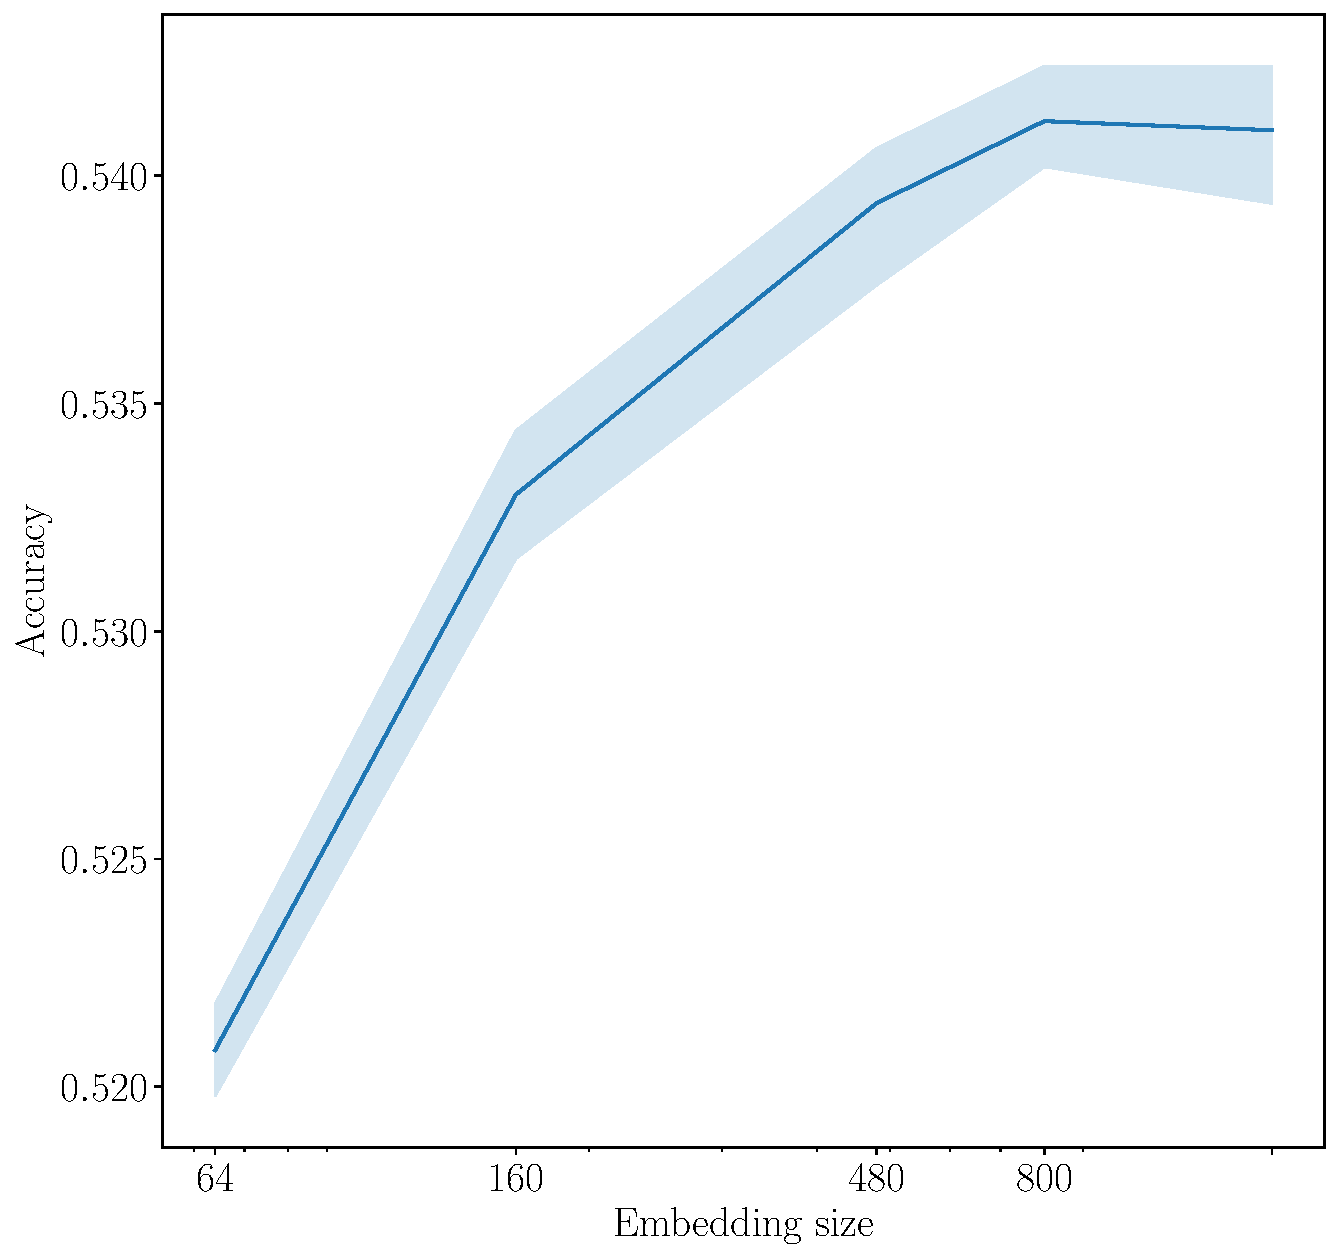
\includegraphics[width=\linewidth]{figures/hidden_size_x5.pdf}
  \end{subfigure}
  \label{fig-emb-dim}
\end{figure*}

\subsubsection{Self-supervised embeddings}

We compared CoLES with baselines described in Section~\ref{sec-baselines} in two scenarios. First, we compared embeddings produced by the CoLES encoder with other types of embeddings and with manually created aggregates by using them as input features of a downstream task model (see Figure~\ref{fig-arch}, Phase 2a). The downstream task model is trained by LightGBM~\citep{Ke2017LightGBMAH} independently from the sequence encoder. As Table~\ref{tab-downstream-res-emb} demonstrates, our method generates sequence embeddings of sequential data that achieve strong performance results in comparison to the case of manually crafted features when used on the downstream tasks.
In particular, Table~\ref{tab-downstream-res-emb} shows that even unsupervised CoLES embeddings perform on par and sometimes even better than hand-crafted features. Also note that CoLES embeddings consistenlty outperform embeddings produced by the other self-supervised baselines on \revised{the four of the five considered datasets}.

\revised{On the scoring dataset, which is significanly larger than the other datasets CoLES, CPC and RTD, significantly outperform hand-crafted features baseline. Since more recent information is more valuable for the credit scoring task CPC, wich is autoregressive method is also effective on this dataset. RTD method is trained on the unusual event detection task is also effective for credit scoring.}

\revised{Simple hand-crafted features can achieve competitive results if the events have a clear structure for designing them. E.g. it is easy to calculate some aggregate statistics per MCC code for the card transactions history. In the commercial settings (which we consider in Section~\ref{sec-commercial}) we've seen different situation: it was hard to develop effective hand-crafted features for the transactions of the legal entities since it is not clear how they can be grouped. We discuss the difference between simple events (card transactions) and more complex events (transactions of the legal entities) at the end of Section~\ref{sec-commercial}.}

\begin{comment}
\begin{table}
\centering
\caption{Quality of unsupervised embeddings as features for the downstream task}
\begin{tabularx}{\linewidth}{Xcccc}

\toprule
\textbf{Method} &
\makecell{\textbf{Age} \\ \small{Accuracy}} &
\makecell{\textbf{Churn} \\ \small{AUROC}} &
\makecell{\textbf{Assess} \\ \small{Accuracy}} &
\makecell{\textbf{Retail} \\ \small{Accuracy}}\\
\midrule

\textbf{Designed features} & $0.631$\tiny{$\pm 0.003$} & $0.825$\tiny{$\pm 0.004$} & \bm{$0.602$}\tiny{$\pm 0.005$} & \bm{$0.547$}\tiny{$\pm 0.001$} \\

\textbf{SOP} & $0.493$\tiny{$\pm 0.002$} & $0.782$\tiny{$\pm 0.005$} & $0.577$\tiny{$\pm 0.002$} & $0.428$\tiny{$\pm 0.001$}\\

\textbf{NSP} & $0.622$\tiny{$\pm 0.004$} & $0.830$\tiny{$\pm 0.004$} & $0.581$\tiny{$\pm 0.003$} & $0.425$\tiny{$\pm 0.002$}\\

\textbf{RTD} & $0.632$\tiny{$\pm 0.002$} & $0.801$\tiny{$\pm 0.004$} & $0.580$\tiny{$\pm 0.003$} & $0.520$\tiny{$\pm 0.001$}\\

\textbf{CPC} & $0.594$\tiny{$\pm 0.002$} & $0.802$\tiny{$\pm 0.003$} & $0.588$\tiny{$\pm 0.002$} & $0.525$\tiny{$\pm 0.001$}\\

\textbf{CoLES} & \bm{$0.638$}\tiny{$\pm 0.007$} & \bm{$0.843$}\tiny{$\pm 0.003$} & $0.601$\tiny{$\pm 0.002$} & $0.539$\tiny{$\pm 0.001$} \\

\bottomrule
\end{tabularx} \\
\small{average test set quality metric and its standard deviation for 5 runs on different folds is shown}
\label{tab-downstream-res-emb}
\end{table}
\end{comment}

\begin{table*}
\centering
\caption{Quality of unsupervised embeddings as features for the downstream task}
\begin{tabularx}{\linewidth}{Xccccc}

\toprule
\textbf{Method} &
\makecell{\textbf{Age} \\ \small{Accuracy}} &
\makecell{\textbf{Churn} \\ \small{AUROC}} &
\makecell{\textbf{Assess} \\ \small{Accuracy}} &
\makecell{\textbf{Retail} \\ \small{Accuracy}} &
\makecell{\revised{\textbf{Scoring}} \\ \small{AUROC}}\\
\midrule

\textbf{Designed features} & $0.631$\tiny{$\pm 0.003$} & $0.825$\tiny{$\pm 0.004$} & \bm{$0.602$}\tiny{$\pm 0.005$} & \bm{$0.547$}\tiny{$\pm 0.001$} & $0.779$\tiny{$\pm 0.001$} \\

\textbf{SOP} & $0.493$\tiny{$\pm 0.002$} & $0.782$\tiny{$\pm 0.005$} & $0.577$\tiny{$\pm 0.002$} & $0.428$\tiny{$\pm 0.001$} & $0.724$\tiny{$\pm 0.001$} \\

\textbf{NSP} & $0.622$\tiny{$\pm 0.004$} & $0.830$\tiny{$\pm 0.004$} & $0.581$\tiny{$\pm 0.003$} & $0.425$\tiny{$\pm 0.002$} & $0.766$\tiny{$\pm 0.001$} \\

\textbf{RTD} & $0.632$\tiny{$\pm 0.002$} & $0.801$\tiny{$\pm 0.004$} & $0.580$\tiny{$\pm 0.003$} & $0.520$\tiny{$\pm 0.001$} & $0.791$\tiny{$\pm 0.001$} \\

\textbf{CPC} & $0.594$\tiny{$\pm 0.002$} & $0.802$\tiny{$\pm 0.003$} & $0.588$\tiny{$\pm 0.002$} & $0.525$\tiny{$\pm 0.001$} & $0.791$\tiny{$\pm 0.001$} \\

\textbf{CoLES} & \bm{$0.638$}\tiny{$\pm 0.007$} & \bm{$0.843$}\tiny{$\pm 0.003$} & $0.601$\tiny{$\pm 0.002$} & $0.539$\tiny{$\pm 0.001$} & \bm{$0.792$}\tiny{$\pm 0.001$} \\

\bottomrule
\end{tabularx} \\
\small{average test set quality metric and its standard deviation for 5 runs on different folds is shown}
\label{tab-downstream-res-emb}
\end{table*}

\subsubsection{Fine-tuned embeddings}

In the second scenario, we fine-tune pre-trained models for specific downstream tasks (see Figure~\ref{fig-arch}, Phase 2b). The models are pre-trained using CoLES and other self-supervised learning approaches and then are additionally trained on the labeled data for the specific task.

\revised{The fine-tuning step is done by adding the classification sub-network $h$ to the pre-trained encoder network $e$ (see Section~\ref{sec-enc-arch}). Both subnetworks are jointly trained on the downstream task target, i. e. the classification sub-network takes encoder output and produces a prediction: $\hat{y} = h(e(x))$. One-layer neural net with softmax activation is used as $h$.}

In addition to the aforementioned baselines, we compare our method with a supervised learning approach where the encoder network $e$ is not pre-trained using self-supervised target.

As Table~\ref{tab-downstream-res} shows, CoLES representations obtained after fine-tuning achieve superior performance on all the considered datasets, outperforming all other methods by significant margins.

\begin{table}
\centering
\caption{Quality of the pre-trained model on the downstream tasks}
\begin{tabularx}{\linewidth}{Xcccc}
\toprule
\textbf{Method} & \makecell{\textbf{Age} \\ \small{Accuracy}} & \makecell{\textbf{Churn} \\ \small{AUROC}} & \makecell{\textbf{Assess} \\ \small{Accuracy}} & \makecell{\textbf{Retail} \\ \small{Accuracy}}\\
\midrule
\textbf{Designed features} & $0.631$\tiny{$\pm 0.003$} & \bm{$0.825$}\tiny{$\pm 0.004$} & $0.602$\tiny{$\pm 0.005$} & $0.547$\tiny{$\pm 0.001$} \\

\textbf{Super\-vised learning} & $0.628$\tiny{$\pm 0.004$} & $0.817$\tiny{$\pm 0.009$} & $0.602$\tiny{$\pm 0.005$} & $0.542$\tiny{$\pm 0.001$}\\

\textbf{RTD pretrain} & $0.635$\tiny{$\pm 0.006$} &  $0.819$\tiny{$\pm 0.005$} & $0.586$\tiny{$\pm 0.003$} & $0.544$\tiny{$\pm 0.002$} \\

\textbf{CPC pretrain} & $0.615$\tiny{$\pm 0.009$} &  $0.810$\tiny{$\pm 0.006$} & $0.606$\tiny{$\pm 0.004$} & $0.549$\tiny{$\pm 0.001$} \\

\textbf{CoLES pretrain} & \bm{$0.644$}\tiny{$\pm 0.004$} & \bm{$0.827$}\tiny{$\pm 0.004$} & \bm{$0.615$}\tiny{$\pm 0.003$} & \bm{$0.552$}\tiny{$\pm 0.001$} \\

\bottomrule
\end{tabularx} \\
\small{average test set quality metric and its standard deviation for 5 runs on different folds is shown}
\label{tab-downstream-res}
\end{table}

\subsubsection{Semi-supervised setup}

Here we study the applicability of our method in scenarios where the amount of labeled examples is limited. We performed a series of experiments where only a random fraction of available labels is used to train the downstream task models. As in the case of the supervised setup, we compare the proposed method with LigthGBM over hand-crafted features, CPC, and supervised learning without pre-training.

The results of this comparison are presented in Figure \ref{fig-semi-main}. Note that the performance improvement of CoLES with respect to supervised-only methods increases as we decrease the portion of labeled examples in the training dataset. Also note that CoLES consistently outperforms CPC for different volumes of labeled data.

\begin{figure*}
  \centering
  \begin{subfigure}{0.25\linewidth}
    \caption{Age group}
    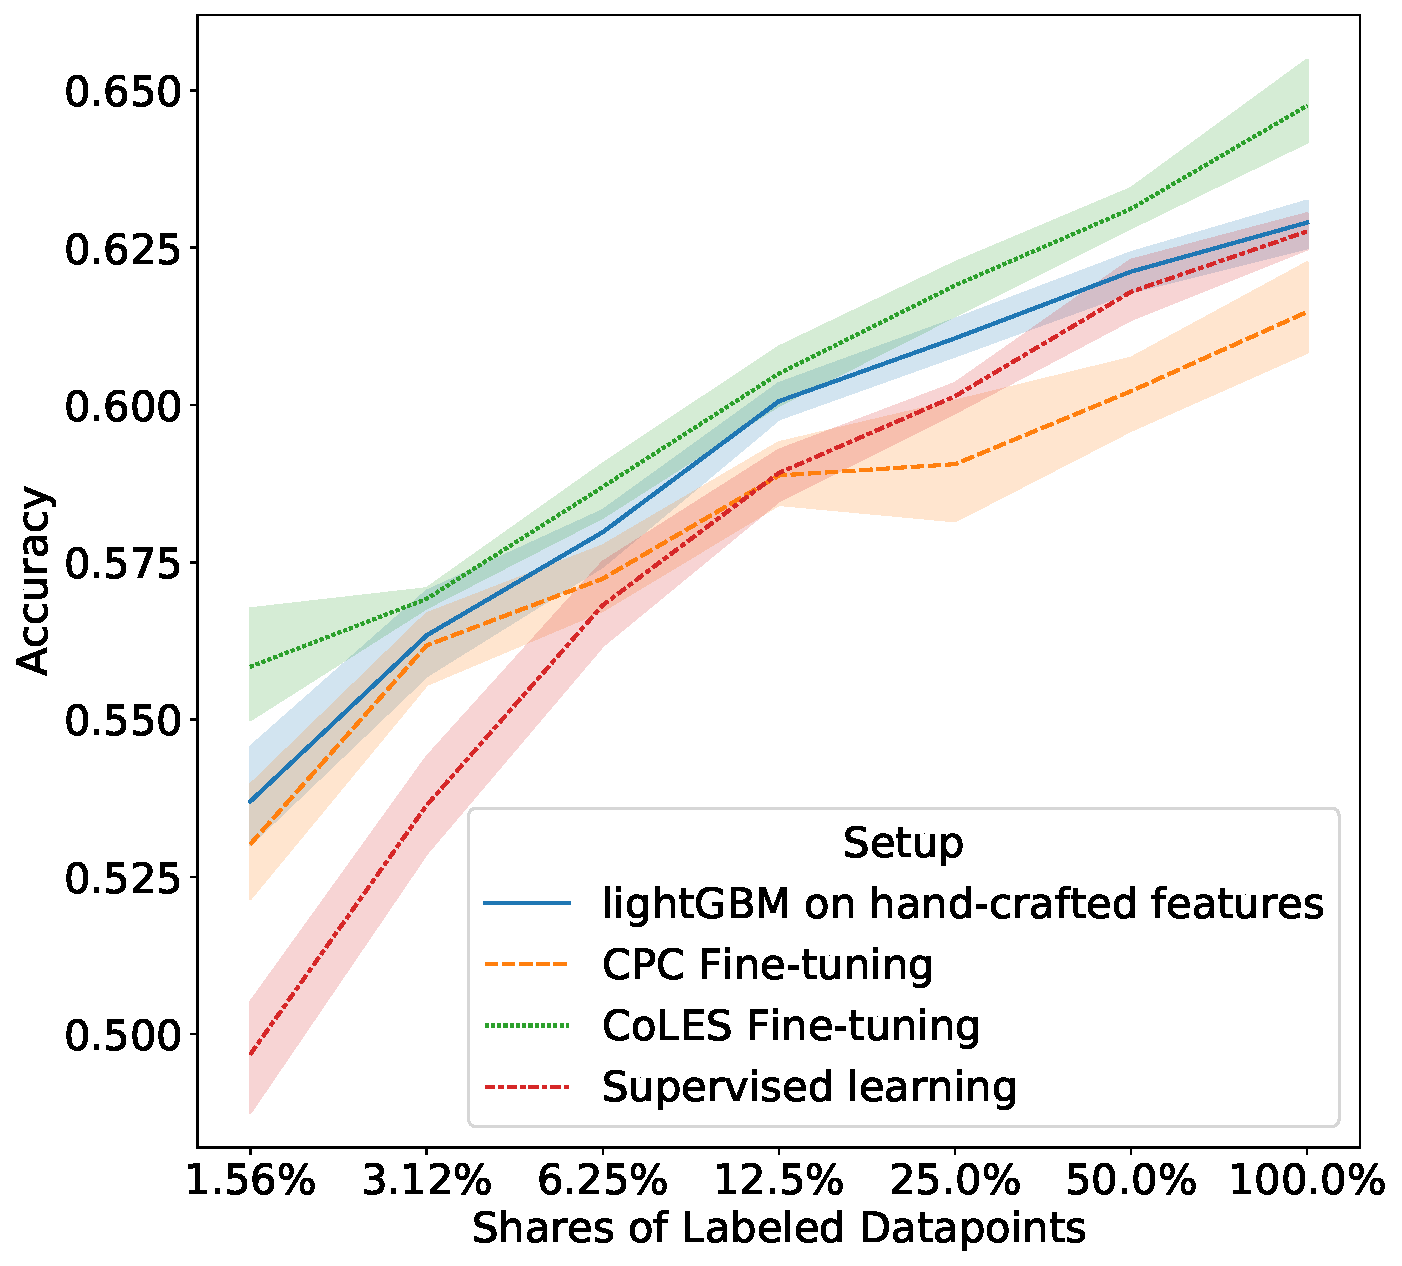
\includegraphics[width=\linewidth]{figures/ss_age_pred_per.pdf}
  \end{subfigure}%
  \begin{subfigure}{0.25\linewidth}
    \caption{Churn}
    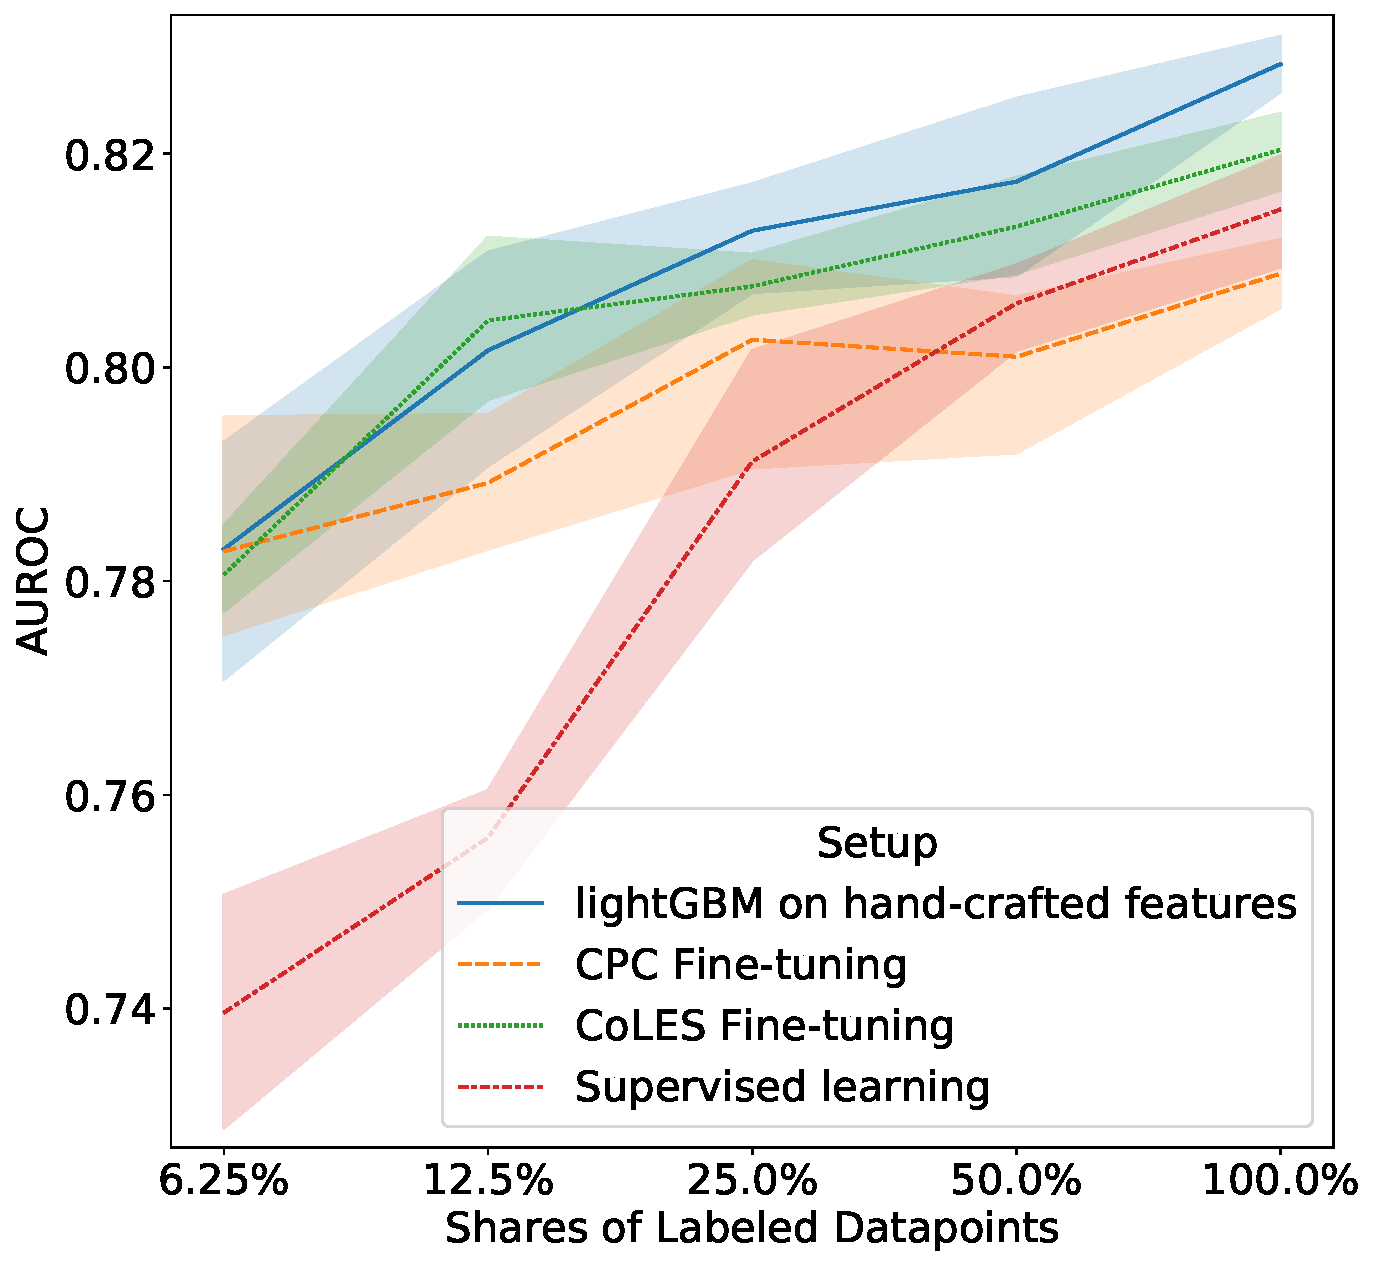
\includegraphics[width=\linewidth]{figures/ss_rosbank_per.pdf}
  \end{subfigure}%
  \begin{subfigure}{0.25\linewidth}
    \caption{Assessment}
    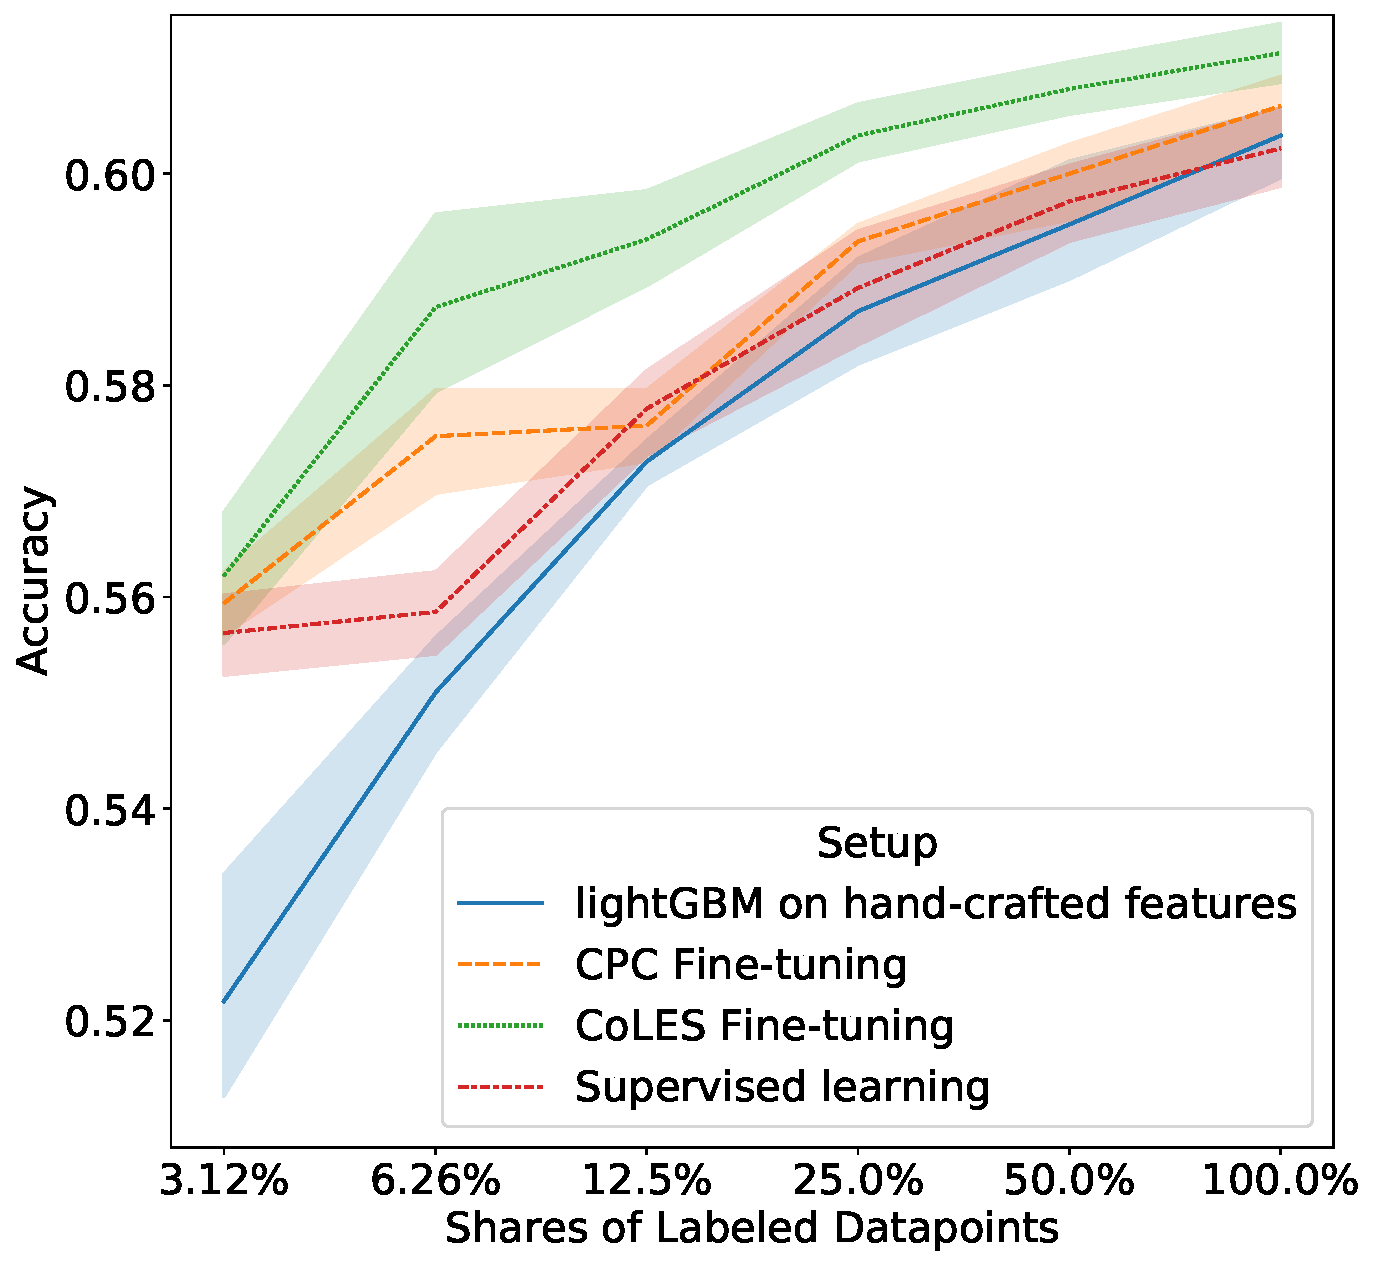
\includegraphics[width=\linewidth]{figures/ss_bowl2019_per.pdf}
  \end{subfigure}%
  \begin{subfigure}{0.25\linewidth}
    \caption{Retail}
    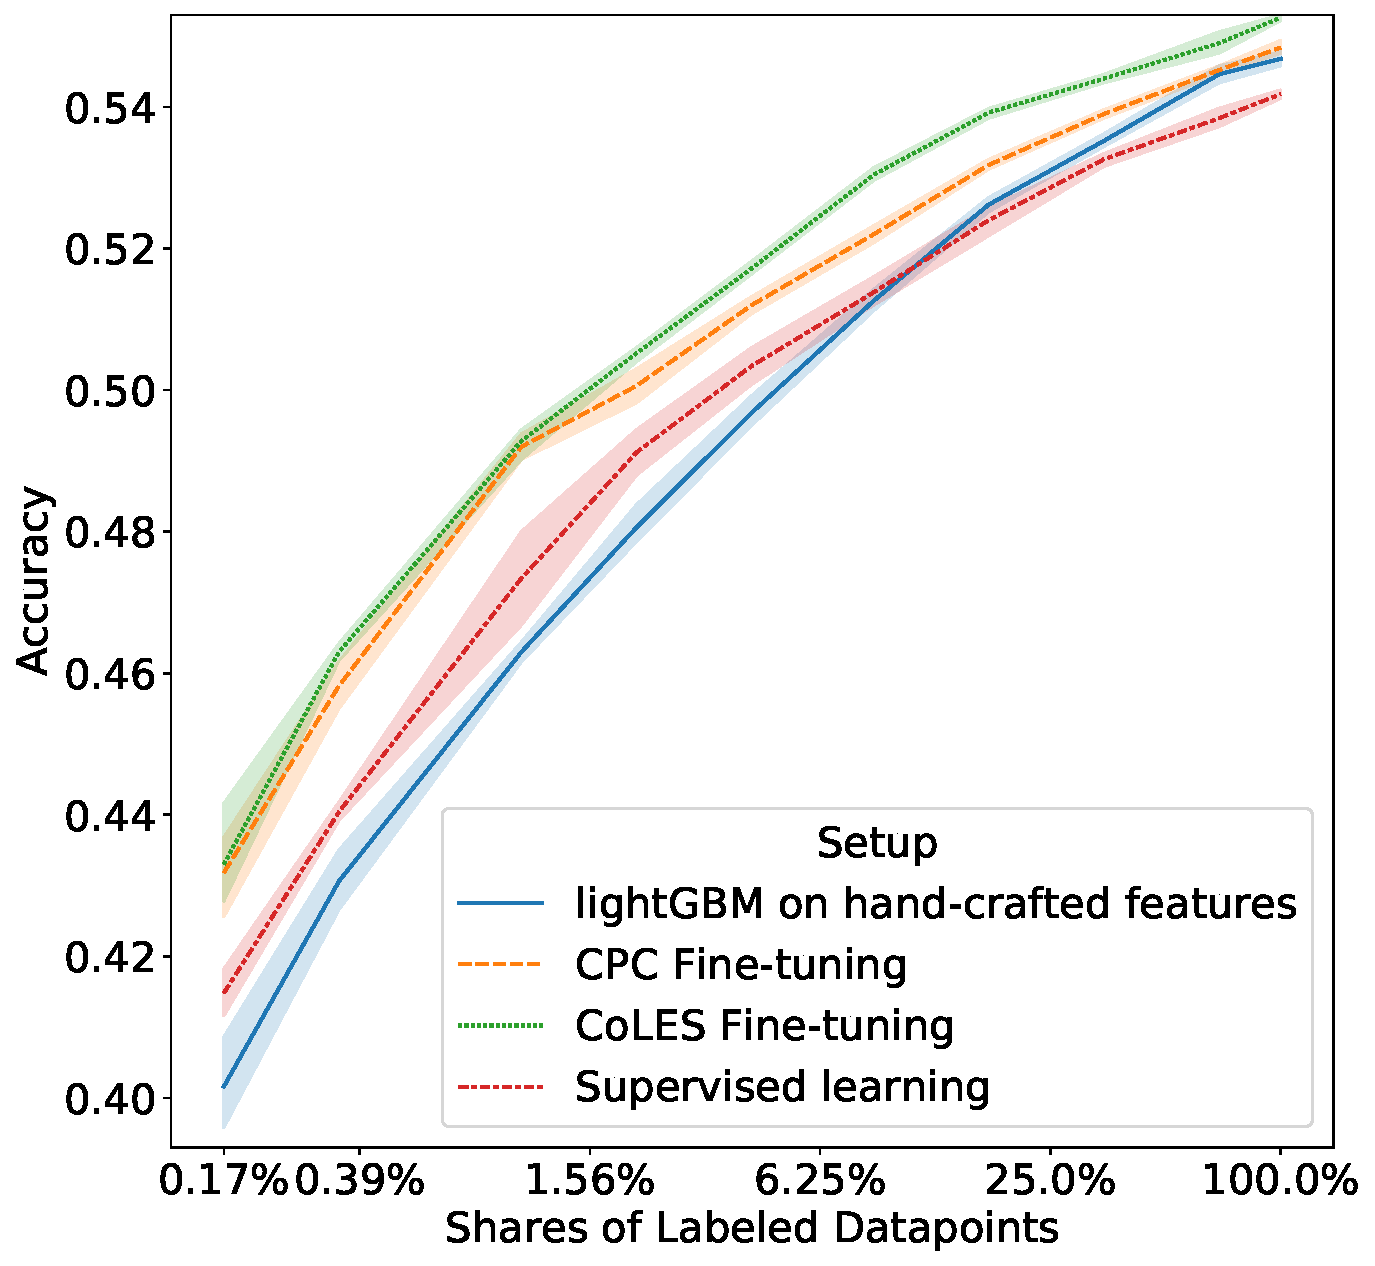
\includegraphics[width=\linewidth]{figures/ss_x5_per.pdf}
  \end{subfigure}
  \caption{Model quality for different dataset sizes} \small{The rightmost point corresponds to all labels and supervised setup.}
  \label{fig-semi-main}
\end{figure*}

\subsection{CoLES Embeddings in Commercial Settings} \label{sec-commercial}

\begin{table}
\centering
\caption{Data structure of the credit card transactions}
\begin{tabular}{llllll}
\toprule
\textbf{Date} & \textbf{Amount} & \textbf{Currency} & \textbf{Country} & \makecell{\textbf{Merchant} \\ \textbf{Type}} \\
\midrule
Jun 21 & 230 & EUR & France & Restaurant \\
Jun 21 & 5 & USD & US & Transportation \\
Jun 22 & 40 & USD & US & \makecell[l]{Household \\ Appliance} \\
\bottomrule
\end{tabular}
\label{tab-tr-data}
\end{table}


\begin{table}
\centering
\caption{Data structure of the money transfers between legal entities}
\begin{tabular}{lllllll}
\toprule
\textbf{Date} & \textbf{Amount} & \textbf{Currency} & \textbf{Sender} & \textbf{Receiver} & \textbf{Type} \\
\midrule
Jul 11 & 20000 & EUR & 1232323 & 6345433 & 23 \\
Jul 11 & 5000 & USD & 5424443 & 1232323 & 12 \\
Jul 12 & 14000 & USD & 1232323 & 5424443 & 14 \\
\bottomrule
\end{tabular}
\small{The information about company business and the company region is encoded in the first letters of the company identifier stored in "Sender" and "Receiver" fields.}
\label{tab-org-tr-data}
\end{table}

Self-supervised CoLES embenddings are widely used in the ecosystem of a large European financial services company.
In particular, we created two types of embeddings: (1) \emph{legal entity embeddings} of the small and medium--size companies,
based on commercial transactions and operational histories of their businesses and (2) \emph{personal embeddings} of individual/retail customers %of the company, their embeddings are%
based on their debit/credit card transactional histories. Table~\ref{tab-tr-data} and Table~\ref{tab-org-tr-data} provide some examples of the transactional data used for building personal and legal entities embeddings. Overall, the dataset of 10 million corporate clients with the mean number of 200 transactions per client was used to train the model for legal entities embeddings, and the dataset of 5 million clients with the mean number of 400 transactions per client was used to train the model for personal embeddings. These two "in-house" commercial datasets are much larger than the public datasets described in Section~\ref{sec-exp}, and this availability of extensive amounts of self-supervised training data allowed us to generate embeddings of significantly higher quality than on the publicly available data.

We performed an extensive evaluation of CoLES embeddings on these in-house datasets by applying them to different downstream modelling tasks.
Legal entity embeddings were applied in the following use cases:
\begin{itemize}
    \item \textbf{Corporate medical insurance lead generation.} In this task, the model should be able to predict client's interest in a corporate medical insurance product.
    \item \textbf{Credit lead generation} for small and medium size businesses. In this task, the model should predict an interest of a company in taking a credit.
    \item \textbf{Credit scoring} for small and medium size businesses. In this task, the model should predict the the probability of a company's default.
    \item \textbf{Holding structure restoration.} In this task, the model should predict if a pair of companies are in the same holding of companies.
    \item \textbf{Fraudulent money transfers monitoring.} In this task, the model is used to estimate the likelihood that a particular transaction is fraudulent.
\end{itemize}
Personal embeddings are applied to the following downstream~tasks:
\begin{itemize}
    \item \textbf{Retail credit scoring.} In this task, the model should estimate the probability of default when a client is taking a retail credit.
    \item \textbf{Customer churn prediction.} In this task, the model should predict the possibility that a client would stop using the company products (cards and deposits).
    \item \textbf{Life insurance lead generation.} In this task, the model should predict an interest in a life insurance product.
\end{itemize}


We considered the following three scenarios in most of these tasks: (1) the baseline scenario, where only the hand-crafted features were used for predictive modelling; (2) the CoLES scenario, where self-supervised embeddings, generated using the propsoed method, subsequently used as features of predictive models; (3) the hybrid (Baseline + CoLES) scenario where both the hand-crafted features and the CoLES embeddings were used for predictive modelling. In all of these three scenarios, we used the LightGBM method~\citep{Ke2017LightGBMAH} for predictive modelling.
In the 1st and the 3rd scenarios, we deployed the existing sets of hand-crafted features previously developed in the organization for the considered use cases (see Section~\ref{sec-hand-features} for some examples of the hand-crafted features).
%These features were partly based on the aggregate statistics of the transaction history and partly on some additional attributes obtained from other data sources.

The results of our experiments are presented in Table~\ref{tab-internal-company} and Table~\ref{tab-internal-person}. We observe a significant increase in model performance thanks to the addition of CoLES embeddings to the hand-crafted features.

Note that it is more difficult to design valuable hand-crafted features for companies than for individual customers. A typical feature is some statistic aggregated over groups of transactions on some level. For example, one can aggregate card transactions of an individual customer on the level of their "merchant type" (MCC) field. On the contrary, it is not clear how to group funds transfers of a company using "receiver" field (see example transfers in Table~\ref{tab-org-tr-data}). It is hard to manually find a perfect level of aggregation for receivers, since they can be grouped in many different ways, e.g., by region, by size, by the type of business, etc. We believe, CoLES is able to automatically learn a suitable aggregation level. This is one of the reasons why legal entity embeddings show better relative improvements with respect to hand-crafted features than personal embeddings in our experiments.

\subsubsection{Deployment details} \label{sec-deployment}

\revised{The application of our method in the production envinronment consists from two parts: the training of encoder neural net (training part) and calculation of embeddings using trained model (inference part). We used only part of the available client data for the training (10 million corporate clients, and 5 million individual clients), but applied the trained model to the all available transactional data which were more than 90 million cards in total. We did not use any of the available distributed training techniques~\citep{Recht2011HogwildAL, Zhao2016FastAP, Kennedy2019APA} during the training part. During the inference part we used popular horizontal scaling scheme, when sequences of the different clients are processed independently on different nodes of the Hadoop cluster. We used Apache Spark for distributed job runnig.}

In order to minimise the efforts of deploying CoLES embeddings inside the company, we used an ETL process for systematic recalculation of embeddings when new transactional data arrives.

In particular, the encoder based on an RNN-type architecture such as GRU~\citep{Cho2014LearningPR} allows to calculate embedding $c_{t+k}$ by updating embedding $c_t$ instead of calculating embedding $c_{t+k}$ from the whole sequence of past events $z_{1:t}$: $c_k = rnn(c_t, z_{t+1:k})$. We use this optimization to reduce the inference time to update already existing client embeddings with new transactional events that occurred after the previous calculation of embeddings. This is possible due to the recurrent nature of RNN-like networks.

Furthermore, compact version of embeddings can be used to minimize their storage (or transfer) volume. To produce the compact version, we discretized the components of the embedding vectors, i.e. we mapped 8-byte float values to the discrete set of values in the range from 0 to 15. After discretization, each component of the embedding vector is stored in 4 bits, hence, a 256-dimensional embedding can be stored in 128 bytes. The discretization operation is partly receiversible, hence, it is still possible to update discretized embedding as discussed in previous paragraph.

\begin{table}
\centering
\caption{Performance comparison of CoLES-based models with the baselines across downstream tasks for the legal entities}
\begin{tabularx}{\linewidth}{Xccc}
\toprule
\textbf{Task} & \textbf{Baseline } & \textbf{CoLES} & \makecell{\textbf{Baseline} \\ \textbf{+ CoLES}} \\ 
\midrule
\textbf{Insurance lead generation} & 0.71 & 0.85 & \textbf{0.85} \\
\textbf{Credit lead generation} & 0.75 & 0.79 & \textbf{0.79} \\
\textbf{Credit scoring} & 0.73 & 0.71 & \textbf{0.77} \\
\textbf{Holding structure restoration} & 0.92 & 0.97 & \textbf{0.97} \\
\textbf{Fraud monitoring} & 0.82 & 0.84 & \textbf{0.85} \\
\bottomrule
\end{tabularx}
\small{Baseline includes both transactional and non-transactional hand-crafted features. AUROC is used as quality metric.}
\label{tab-internal-company}
\end{table}



\begin{table}
\centering
\caption{Performance comparison of CoLES-based models with the baselines across downstream tasks for the retail customers}
\begin{tabularx}{\linewidth}{Xccc}
\toprule
\textbf{Task } & \textbf{Baseline} & \textbf{CoLES} & \makecell{\textbf{Baseline}\\\textbf{+ CoLES}} \\
\midrule
\textbf{Retail credit scoring} & 0.88 & 0.87 & \textbf{0.92} \\
\textbf{Customer churn} & 0.74 & 0.65 & \textbf{0.76} \\
%\textbf{Telehealth lead generation} & 0.82 & 0.86 & 0.87 \\
%\textbf{Company positive recommendation prediction} & 0.62 & & 0.65 \\
\textbf{Insurance lead generation} & 0.75 & 0.74 & \textbf{0.78} \\ %Life insurance
\bottomrule
\end{tabularx}

\small{Baseline includes both transactional and non-transactional hand-crafted features. AUROC is used as quality metric.}
\label{tab-internal-person}
\end{table}


\section{Conclusions} \label{sec-conclusions}

In this paper, we present \emph{Contrastive Learning for Event Sequences (CoLES)}, a novel self-supervised method for building embeddings of discrete event sequences.
In particular, the CoLES method can be effectively
%used for pre-training neural networks in semi-supervised settings. It can also be
used to produce embeddings of complex event sequences that can be effectively used in various downstream tasks.

We empirically demonstrate that our approach achieves strong performance results on several downstream tasks and consistently outperforms both classical machine learning baselines on hand-crafted features, as well as on other  previously introduced  self-supervised and semi-supervised learning baselines adapted to the event sequence domain.
In the semi-supervised setting, where the number of labeled data is limited, our method demonstrates even stronger results: the lesser is the labeled data, the larger is the performance margin between CoLES and the supervised-only methods.
Finally, we demonstrated superior performance of CoLES in several production-level applications internally used in our financial services company.

Furthermore, the proposed method of generating embeddings is very useful in production environments since pre-calculated embeddings can be easily used for different downstream tasks \emph{without} performing complex and time-consuming computations on the raw event data.
%Moreover, it is even possible to incrementally update the already calculated embeddings when new data arrives for some encoder architectures, as is shown in Section~\ref{sec-deployment}, which is important in many production environments.

More generally, the proposed method can be applied to the event sequence data that is extensively used by the core businesses of many large companies, including financial institutions, internet companies, retail and telecommunications.

%!!! SECTION IS REMOVED
\begin{comment}

\section*{Broader Impact}

This paper focused on developing a general novel contrastive learning method for the task of self-supervised learning for the discrete event sequences. Therefore, it can be applied to a broad range of practical applications, many of them having strong social and business impacts, such as educational applications dealing with logs of educational activities of  students, security applications dealing with logs of internet access activities and system logs protecting users from various types of malicious cyber-attacks, logs of online games, retail purchase histories, bank transactions and various other types of sequences. 

Furthermore, our method has strong fairness mechanisms built into it since it focuses on the analysis of the granular event sequences and, therefore, does not have to deal with the problem of biased decisions and predictions stemming from poorly computed aggregate data leading to various types of social biases.

Another advantage of using event sequence based embeddings, instead of the raw explicit event data, is that it is exceptionally difficult to restore the exact input sequence from its embeddings due to the fact, that lots of information is dropped during the transformation to embeddings. Therefore, the usage of embeddings leads to better privacy and data security for the end-users than when working directly with the raw event data, and all this is achieved without sacrificing valuable information for downstream tasks.
\end{comment}

\bibliographystyle{ACM-Reference-Format}
\bibliography{sigmod2022}

%!!! APPENDIX IS REMOVED
\begin{comment}

\clearpage

\appendix

\section{Pair distance calculation} \label{app-sec-pair-dist}

In order to select negative samples, we need to compute pair-wise distance between all possible pairs of embedding vectors of a batch. For the purpose of making this procedure more computationally effective we perform normalization of the embedding vectors, i.e. project them on a hyper-sphere of unit radius. Since $D(A,B) = \sqrt{\sum_i(A_i - B_i)^2} = \sqrt{\sum_i A_i^2 + \sum_i B_i^2 - 2\sum_i A_i B_i} $ and $||A||= ||B||=1$, to compute the euclidean distance we only need to compute: $\sqrt{2 - 2(A \cdot B)}$.

To compute the dot product between all pairs in a batch we just need to multiply the matrix of all embedding vectors of a batch by itself transposed, which is a highly optimized computational procedure in most modern deep learning frameworks. Hence, the computational complexity of the negative pair selection is $O(n^2h)$ where $h$ is the size of the output embeddings and $n$ is the size of the batch.

\section{Theoretical analysis} \label{sec-theory}

Assume that process $\{X_e(t)\}_{t=1}^{T_e}$ is a segment of a latent process $\{\widehat{X}_e(t)\}_{t=1}^{\infty}$, which generates sequence of all events in the potentially infinite life of entity $e$. That is, we assume that $X_e(t)=\widehat{X}_e(t+s_e)$ for some random starting point $s_e\in \{0,1,\ldots\}$ and horizon $T_e$. Thus we observe, in our data, segment $[s_e+1,s_e+T_e]$ of the life of $e$. We also make the following Assumptions:
\begin{enumerate}
    \item Process $\{\widehat{X}_e(t)\}_{t=1}^{\infty}$ is cyclostationary (in the strict sense)~\citep{Gardner2006Cyclostationarity} with some period $\widehat{T}$.
    \item Starting $s_e$ is independent, and the distribution of $(s_e \mod \widehat{T})$ is uniform over $[0,\widehat{T}-1]$.
    \item Horizon $T_e$ is independent and follows a power--law distribution on $[m,\infty]$.
\end{enumerate}
These assumptions correspond to a scenario where some persons become clients of a service at a random moment and for some random time span and their behaviour obey some periodicity.    %First assumption is $\ldots$ 
\begin{thm}\label{thm:distribution}
If sequences $\{x_e(t)\}$ in the dataset are generated from latent processes $\{\widehat{X}_e(t)\}$ as described above with a lower bound $m$ for the length of a sequence $\{x_e(t)\}$, then sub-sequences obtained by Algorithm~\ref{alg-slce-ss} from $\{x_e(t)\}$ follow the same distribution as $\{x_e(t)\}$ up to a slight alteration of the distribution of the length $T_e$. Namely, if $T_e$ follows power law with an exponent $\alpha <-1$, then the density function for the length $T'_e$ of a sub-sequence satisfy 
\begin{multline}\label{probability_ratio}
    \left (\frac{m-1}{m}\right )^{-\alpha} p(T_e=k)\leq p(T'_e=k) \leq \left(\frac{k}{k-1/2}\right )^{-\alpha} p(T_e=k)  \quad \\ \mbox{for any } k\in [m,\infty].
\end{multline}
\end{thm}
This theorem means that a sub-sequence obtained by Algorithm~\ref{alg-slce-ss} is a representative sample of entity~$e$ and follows its latent distribution $P_e$. Combining this result with generalization guarantees proved for setting with explicitly observed positive pairs~(\cite{Saunshi2019ICML}), we obtain theoretical background for our implicit self-supervised setting.   
%Further in this paper, we empirically examine whether pairs of such sub-sequences are useful for contrastive learning-based self-supervision.
See Appendix~\ref{app-sec-proof} for the proof of Theorem~\ref{thm:distribution}.

\section{Proof of Theorem 1} \label{app-sec-proof}

In this section, we provide proof of Theorem 1 (Section~\ref{sec-theory}) that justifies the Random Slices sub-sequence generation strategy proposed in the paper.

%First, we give the statement of Theorem~1 for convenience.

%Assume that process $\{X_e(t)\}_{t=1}^{T_e}$ is a segment of a latent process $\{\widehat{X}_e(t)\}_{t=1}^{\infty}$, which generates sequence of all events in the potentially infinite life of entity $e$. That is, we assume that $X_e(t)=\widehat{X}_e(t+s_e)$ for some random starting point $s_e\in \{0,1,\ldots\}$ and horizon $T_e$. Thus we observe, in our data, segment $[s_e+1,s_e+T_e]$ of the life of $e$. We also make the following Assumptions:
%\begin{enumerate}
%    \item Process $\{\widehat{X}_e(t)\}_{t=1}^{\infty}$ is cyclostationary (in the strict sense)~\citep{Gardner2006Cyclostationarity} with some period $\widehat{T}$.
%    \item Starting $s_e$ is independent, and the distribution of $(s_e \mod \widehat{T})$ is uniform over $[0,\widehat{T}-1]$.
%    \item Horizon $T_e$ is independent and follows a power--law distribution on $[m,\infty]$.
%\end{enumerate}
%\begin{thm}
%If sequences $\{x_e(t)\}$ in the dataset are samples of processes $\{X_e(t)\}$, then sub-sequences obtained by the Random Slices generation strategy from $\{x_e(t)\}$ follow the same distribution as $\{x_e(t)\}$ up to a slight alteration of the distribution of the horizon $T_e$. Namely, if $T_e$ follows power law with an exponent $\alpha <-1$, then the density function for the length $T'_e$ of a sub-sequence satisfy 
%\begin{equation}\label{probability_ratio}
%\P(T'_e=k)/\P(T_e=k)\in \left [\left (\frac{m-1}{m}\right %)^{-\alpha},\left (\frac{k}{k-1/2}\right )^{-\alpha}\right %].    
%\end{equation}

%\end{thm}

\begin{proof}
First, we state the following straightforward lemma:
\begin{lem}\label{stationary}
Let a stochastic process $\{Y(t)\}_{t=1}^{\infty}$ be a shift of another stochastic process $\{\widehat{Y}(t)\}_{t=1}^{\infty}$ by independent random time $s$, i.e. $Y(t) = \widehat{Y}(t+s)$ with integer $s\geq 0$. If process $\{\widehat{Y}(t)\}_{t=1}^{\infty}$ is cyclostationary with period $\widehat{T}$ and $(s_e \mod \widehat{T})$ is uniform over $[0,\widehat{T}-1]$, then process $\{Y(t)\}_{t=1}^{\infty}$ is stationary.
\end{lem}
Lemma~\ref{stationary} implies that process $\{X_e(t)\}_{t=1}^{T_e}$ is stationary, and all its segments $\{X_e(t)\}_{t=s'+1}^{T'_e+s'}$ of a given length $T'_e$ define the same distribution over sequences as its starting segment $\{X_e(t)\}_{t=1}^{T'_e}$ does. Furthermore, integrating over $s'$, we conclude that the conditional distribution of a sub-sequence obtained via Random Slices generation strategy given its length $T'_e$ follows the process $\{X_e(t)\}_{t=1}^{T'_e}$. To finish the proof, it remains to prove Equation~\ref{probability_ratio}.

Assume $\P(T_e=k)\propto k^{\alpha}$ for $k\in [m,\infty]$. By the law of total probability, we have $\P(T'_e=k_0)= \sum_{k}\P(T_e=k)\P(T'_e=k_0\mid T_e=k)$, that is,
$$
\P(T'_e=k_0) = C \sum_{k=k_0}^{\infty} k^{\alpha-1},
$$
where $C$ is the normalization constant. To estimate the sum of the series, notice that
\begin{equation}\label{int_inequal}
\int_{k_0-\frac{1}{2}}^\infty x^{\alpha-1} dx > \sum_{k=k_0}^{\infty} k^{\alpha-1} > \int_{k_0}^\infty x^{\alpha-1} dx,    
\end{equation}
where the former inequality follows from the fact that $\int_{k-1/2}^{k+1/2} x^{\alpha-1}> k^{\alpha-1}$ as long as function $f(x)=x^{\alpha-1}$ is convex. After integration, we rewrite Equation~\ref{int_inequal} as follows:
\begin{equation}\label{inequal}
\frac{-1}{\alpha} \left ( k_0-\frac{1}{2}\right )^{\alpha} > \sum_{k=k_0}^{\infty} k^{\alpha-1} > \frac{-1}{\alpha} k_0^{\alpha}. \end{equation}
Using these inequalities, we obtain the upper bound for $\P(T'_e=k)%/\P(T_e=k)
$ in the following way:
\begin{multline*}
\P(T'_e=k_0) = \sum_{k=k_0}^{\infty} k^{\alpha-1} / \sum_{l=m}^\infty \sum_{k=l}^{\infty} k^{\alpha-1} < \\
< \frac{-1}{\alpha} \left ( k_0-\frac{1}{2}\right )^{\alpha} / \sum_{l=m}^\infty \frac{-1}{\alpha} l^{\alpha} = \\
=\left (\frac{k_0}{k_0-1/2}\right )^{-\alpha} k_0^\alpha/\sum_{l=m}^\infty l^{\alpha} = \left (\frac{k_0}{k_0-1/2}\right )^{-\alpha} \P(T_e=k_0).
\end{multline*}
At last, the lower bound for $\P(T'_e=k)%/\P(T_e=k)
$ can be obtained using Equation~\ref{inequal} as follows:
\begin{multline*}
\P(T'_e=k_0) = \sum_{k=k_0}^{\infty} k^{\alpha-1} / \sum_{l=m}^\infty \sum_{k=l}^{\infty} k^{\alpha-1} > k_0^{\alpha} / \sum_{l=m}^\infty  \left (l-\frac{1}{2}\right )^{\alpha} > \\
> \left (\frac{m-1/2}{m}\right )^{-\alpha} k_0^\alpha/\sum_{l=m}^\infty l^{\alpha} = \left (\frac{m-1/2}{m}\right )^{-\alpha} \P(T_e=k_0).
\end{multline*}
The latter inequality in these calculations follows from the fact that $\left (\frac{l-\frac{1}{2}}{l}\right )^{\alpha}<\left (\frac{m-\frac{1}{2}}{m}\right )^{\alpha}$ for $l>m$.

\end{proof}

\section{Data properties} \label{app-sec-data}

To check that sequence lengths of the considered datasets follow the power-low distribution we measured their distribution of lengths. As Figure~\ref{fig-seq-len} shows, the event sequence length distribution is close to the power-law distribution for every considered dataset.

\begin{figure}
  \centering
  \caption{Event sequence length distribution}
  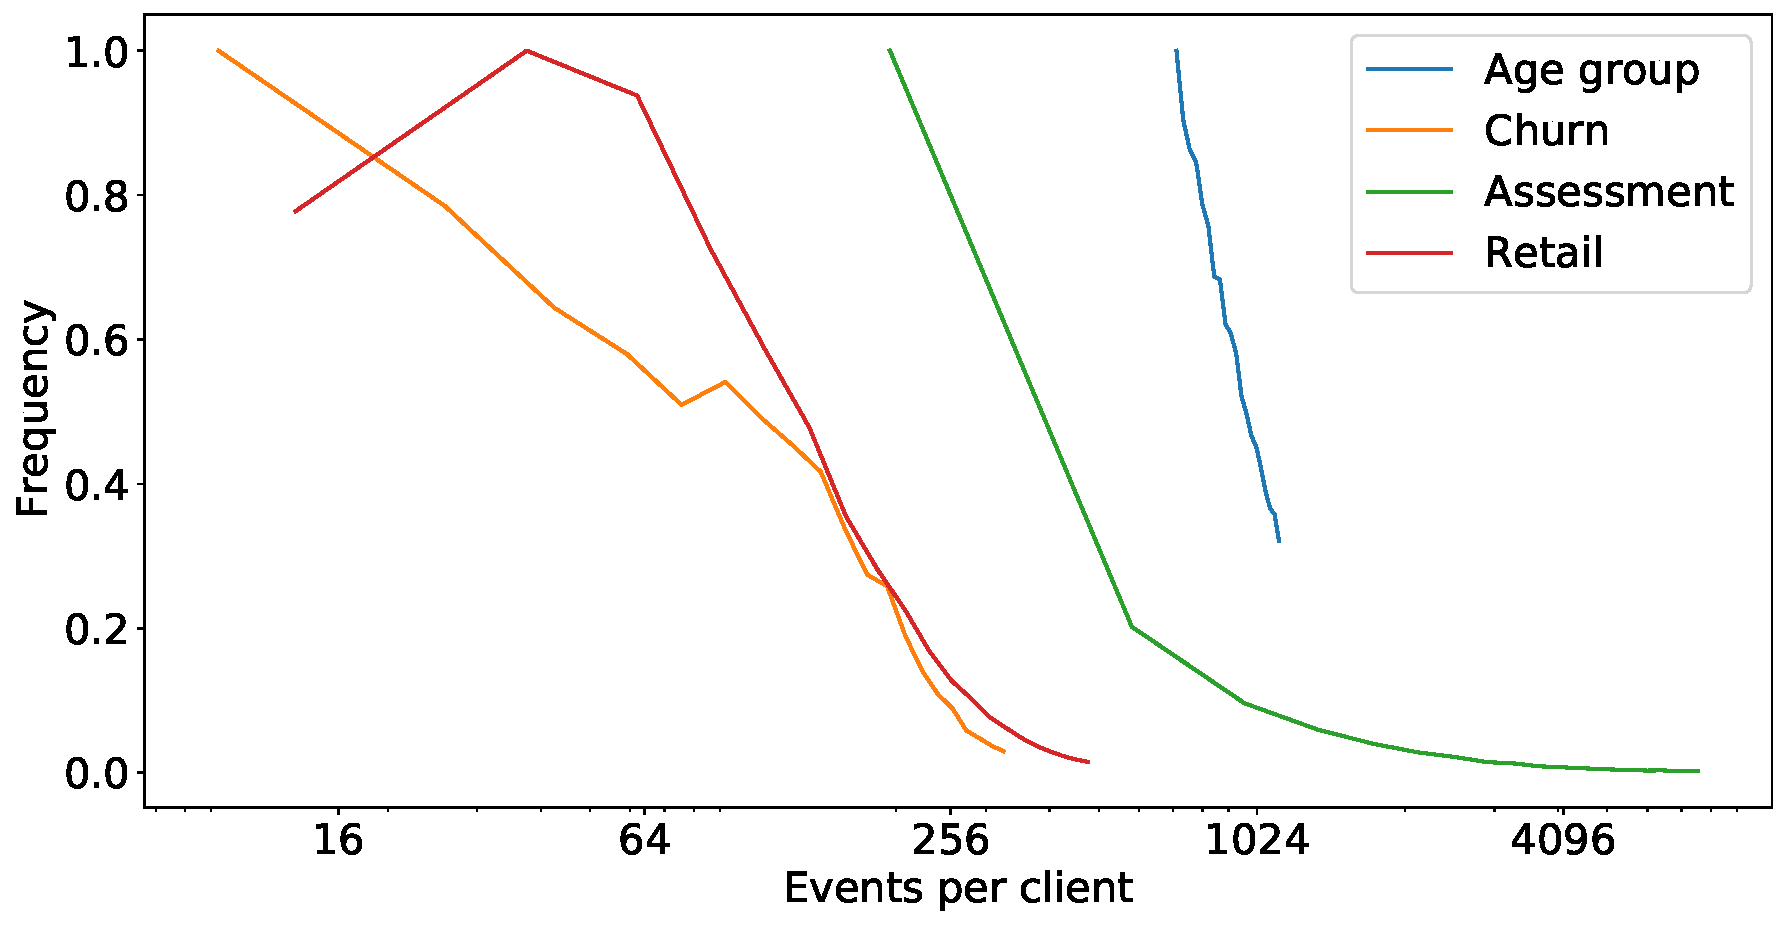
\includegraphics[width=\linewidth]{figures/all_scenario_events_per_client.pdf}
  \label{fig-seq-len}
\end{figure}

\section{Experiment setup} \label{app-sec-exp-setup}

For all methods, a random search on 5-fold cross-validation over the train set is used for hyper-parameter selection. The hyper-parameters with the best out-of-fold performance on the train set are then chosen. The final set of hyper-parameters used for CoLES is shown in Table \ref{tab-hyper}. The number of sub-sequences generated for each sequence was always 5 for each dataset.

\begin{table}
\centering
\caption{Hyper-parameters for CoLES training}
\begin{tabularx}{\linewidth}{Xcccc}
\toprule
\textbf{Dataset} & \textbf{Age group} & \textbf{Churn} & \textbf{Assessment} & \textbf{Retail} \\
\midrule
\textbf{Output size} & 800 & 1024 & 100 & 800 \\
\textbf{Learning rate} & 0.001 & 0.004 & 0.002 & 0.002 \\
\textbf{N samples in batch} & 64 & 128 & 256 & 256 \\
\textbf{N epochs} & 150 & 60 & 100 & 30 \\
\textbf{Min sequence length} & 25 & 15 & 100 & 30 \\
\textbf{Max sequence length} & 200 & 150 & 500 & 180 \\
\textbf{Encoder} & GRU & LSTM & GRU & GRU \\
\bottomrule
\end{tabularx}
\label{tab-hyper}
\end{table}

\subsection{Hand-crafted features} \label{app-sec-hand}

Here we describe the details of producing hand-crafted features. All attributes of each transaction are either numerical (e. g. amount) or categorical (e.g. merchant type (MCC code), transaction type, etc.). 
For the numerical type of attribute we apply aggregation functions, such as 'sum', 'mean', 'std', 'min', 'max', over all transactions per user. For example, if we apply 'sum' for the numerical field 'amount' we obtain a feature 'sum of all transaction amounts per user'. 
For the categorical type of attribute we apply aggregation functions in a slightly different way. For each unique value of categorical attribute we apply aggregation functions, such as 'count', 'mean', 'std' over all transactions per user' numerical attribute. For example, if we apply 'mean' for the numerical attribute 'amount' grouped by categorical attribute 'MCC code' we obtain a feature 'mean amount of all transactions for each MCC code per user'. 
For example, for age prediction task we have one categorical attribute (small group) with 200 unique values, combining it with amount we can produce $200 * 3$ features ('group0 x amount x count',  'group1 x amount x count', ..., 'group199 x amount x count', 'group0 x amount x mean', ...). In total we use approx 605 features for this task. % For gender prediction task we have two categorical features: 'MCC code' with approx 200 unique values and 'tr type' with approx 100 unique values. So in total we use $200 * 3 + 100 * 3 + 5 = 905$ features.
Note, that hand-crafted features contain information about user spending profile but omit information about transactions temporal order.

\section{Results} \label{app-sec-res}

\subsection{Semi-supervised setup} \label{app-sec-semi}

To evaluate our method in case of the restricted amount of labeled data, we use only part of the available target labels for the semi-supervised experiment, see Section~\ref{sec-res} for details. As in the case of the supervised setup, we compare the proposed method with LigthGBM over hand-crafted features, CPC, and supervised learning without pre-training. In figure \ref{fig-semi} we provide learning curves for all considered datasets.

\begin{figure}
  \centering
  \begin{subfigure}{0.5\linewidth}
    \caption{Age group}
    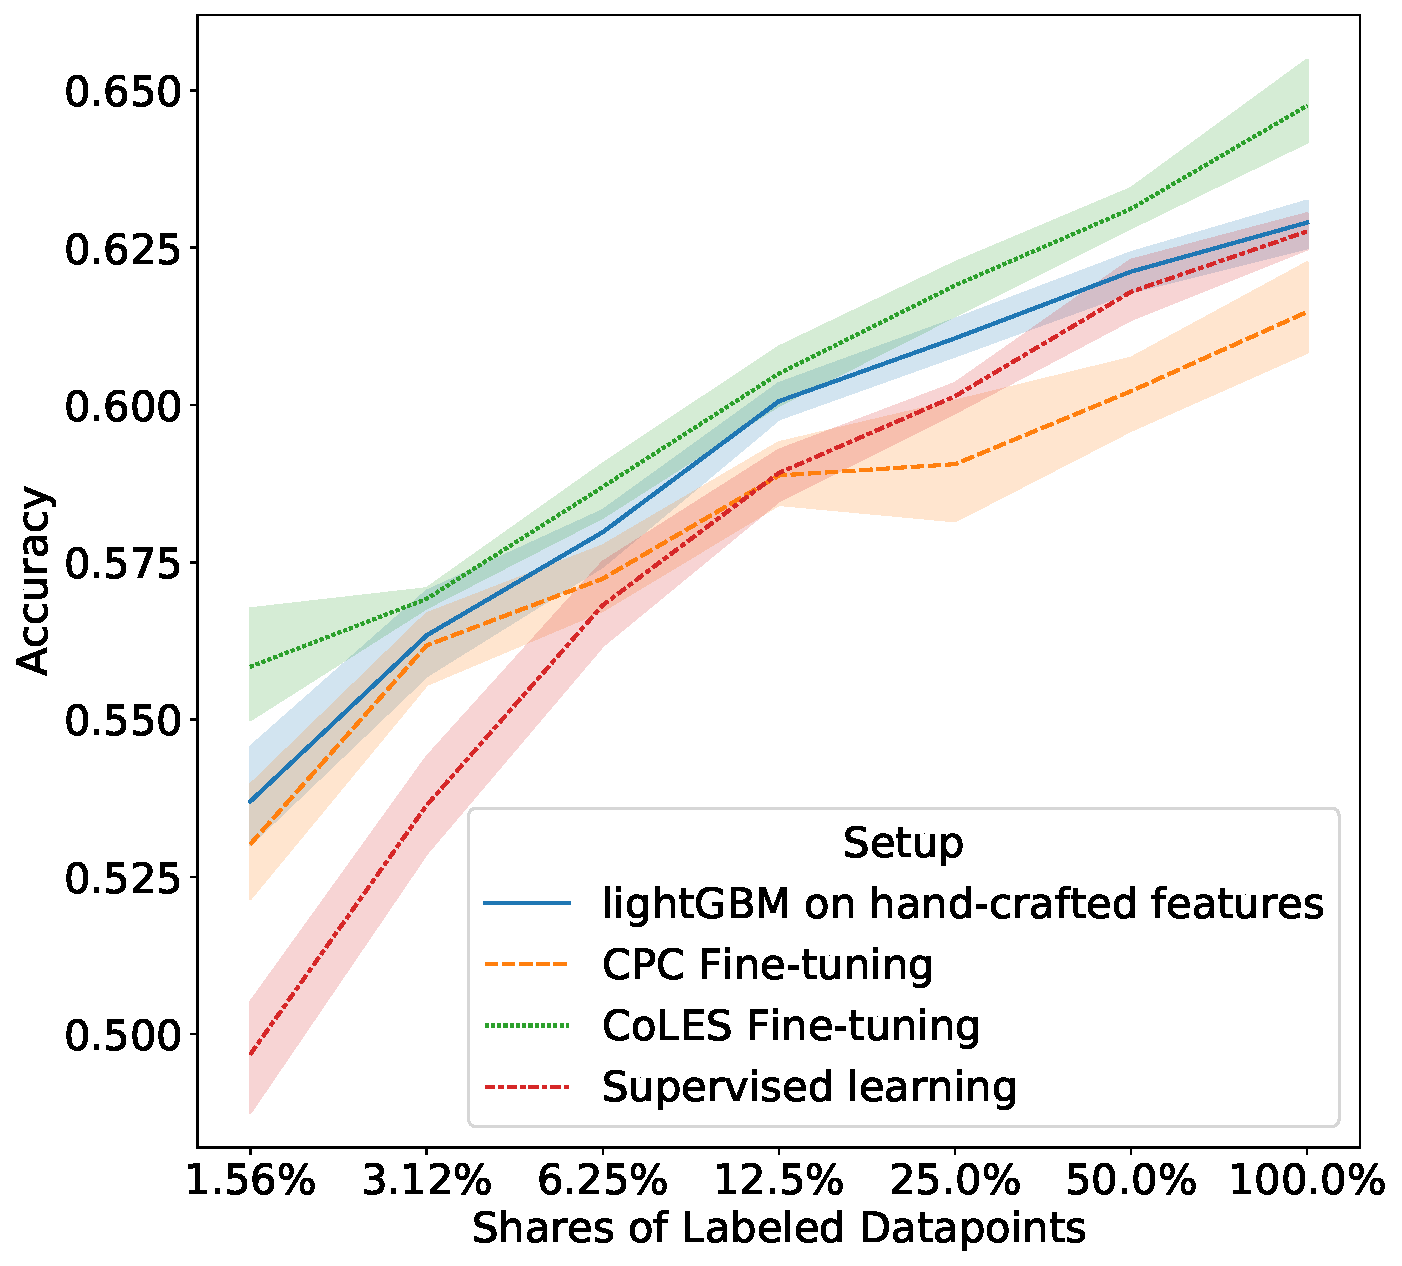
\includegraphics[width=\linewidth]{figures/ss_age_pred_per.pdf}
    \label{fig-semi-age2}
  \end{subfigure}%
  \begin{subfigure}{0.5\linewidth}
    \caption{Churn}
    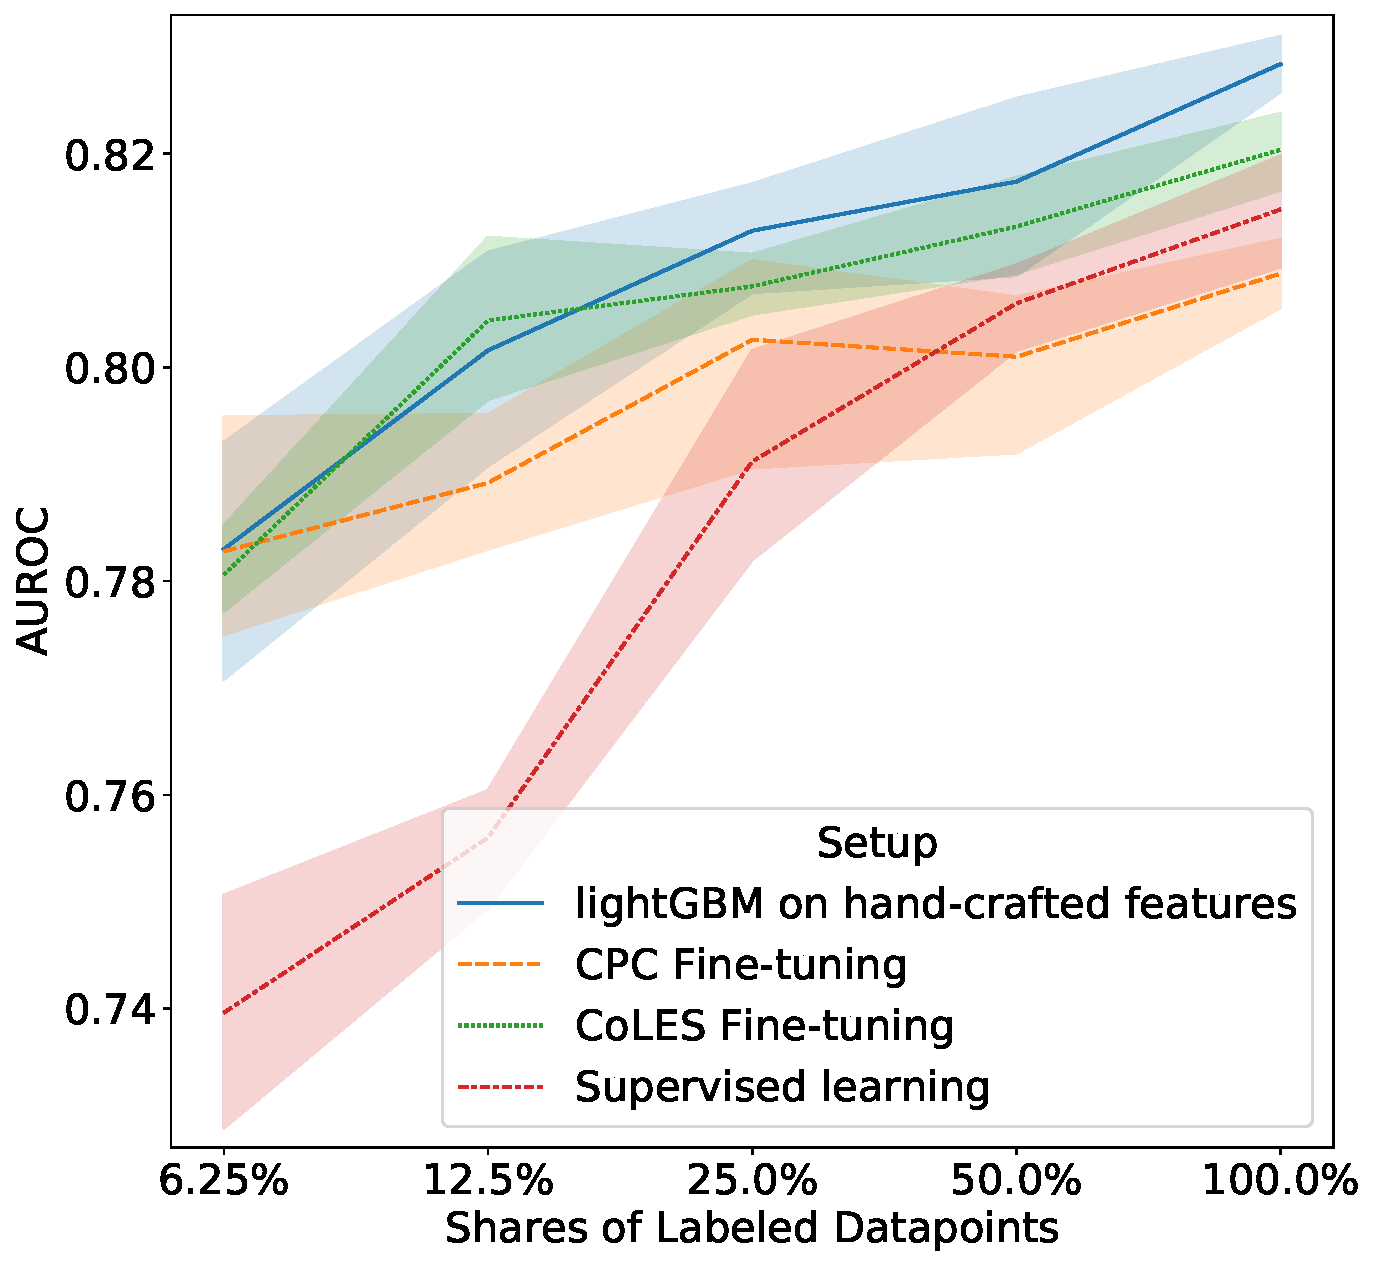
\includegraphics[width=\linewidth]{figures/ss_rosbank_per.pdf}
    \label{fig-semi-churn}
  \end{subfigure}
  \begin{subfigure}{0.5\linewidth}
    \caption{Assessment}
    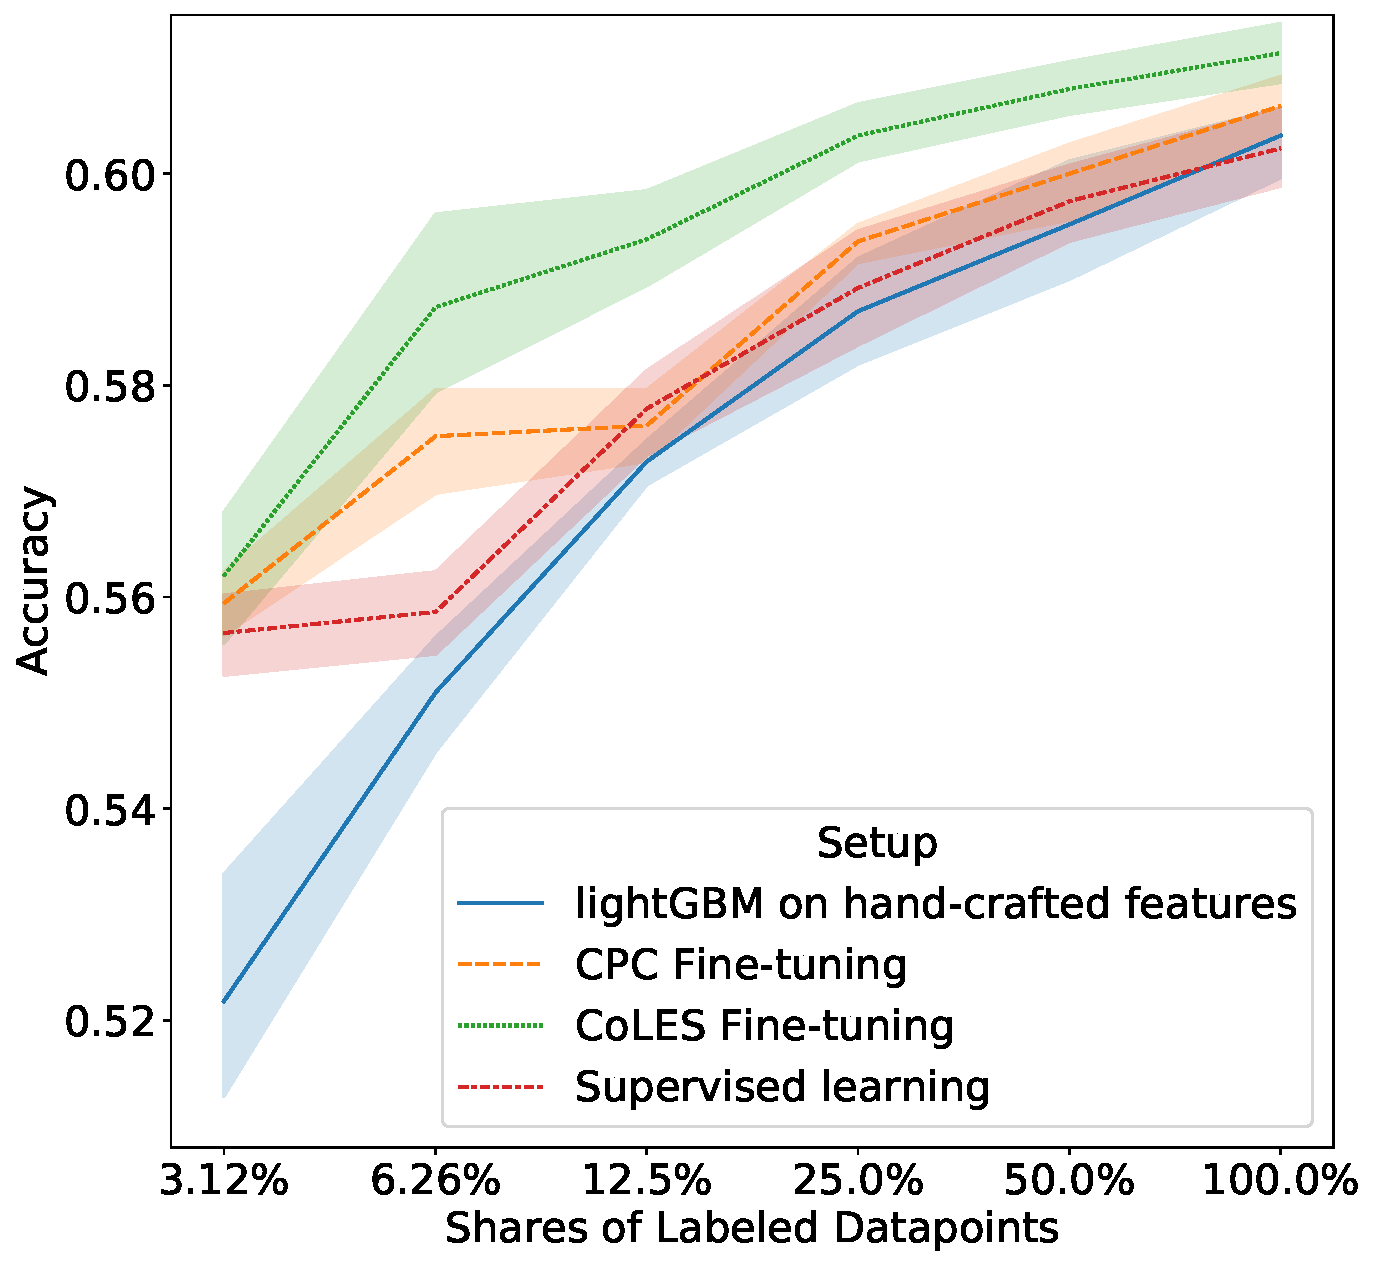
\includegraphics[width=\linewidth]{figures/ss_bowl2019_per.pdf}
    \label{fig-semi-assessment2}
  \end{subfigure}%
  \begin{subfigure}{0.5\linewidth}
    \caption{Retail}
    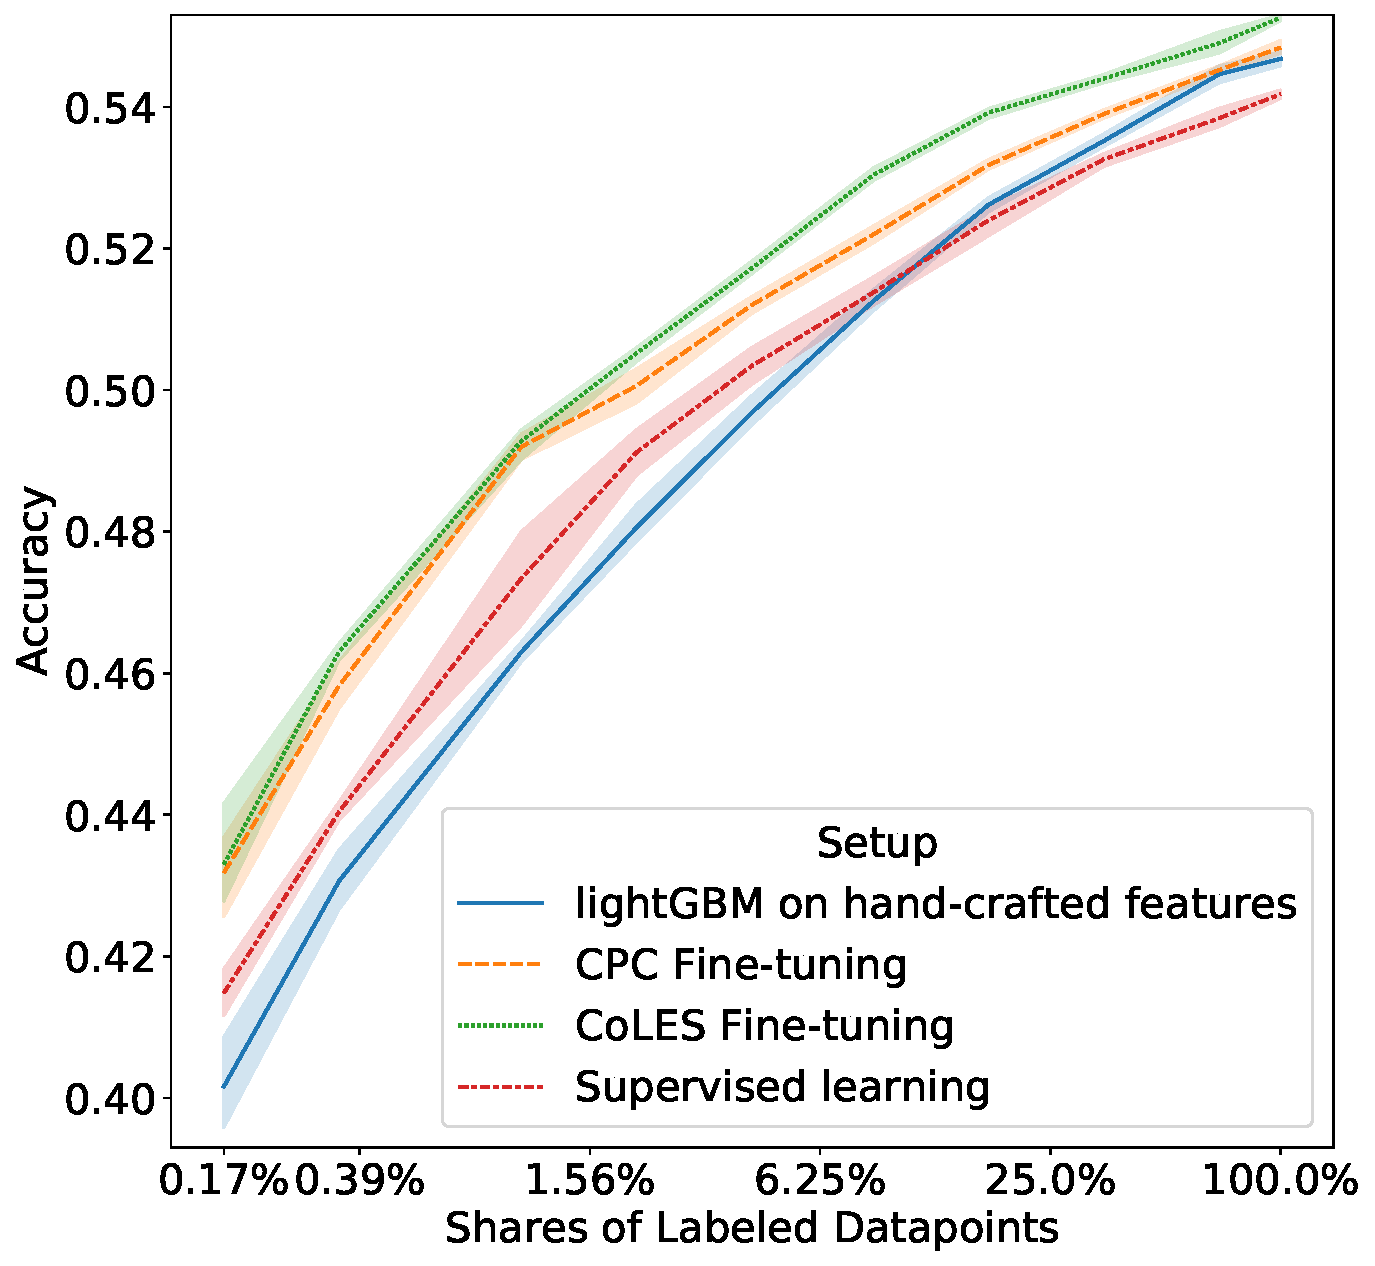
\includegraphics[width=\linewidth]{figures/ss_x5_per.pdf}
    \label{fig-semi-retail}
  \end{subfigure}
  \caption{Model quality for different dataset sizes} \small{The rightmost point corresponds to all labels and supervised setup.}
  \label{fig-semi}
\end{figure}

\subsection{Embedding visualization} \label{app-sec-vis}

In order to visualize CoLES embeddings in 2-dimensional space, we applied tSNE transformation~\citep{Maaten2008VisualizingDU} on them. tSNE transforms high--dimensional space to low--dimensional based on local relationships between points, so neighbor vectors in high-dimensional embedding space are pushed to be close in 2-dimensional space. We colorized 2-dimensional vectors using the target values of the datasets.

Note, that embeddings was learned in a fully self-supervised way from raw user transactions without any target information. The sequence of transactions represent user' behavior, thus the CoLES model captures behavioral patterns and outputs embeddings of users with similar patterns nearby.
As shown below, local clusters in embedding space correspond to the distribution of user's attributes either age or churn fact.

tSNE vectors from the age prediction dataset are presented in Figure \ref{fig-tsne-age2}. We can observe 4 clusters: clusters for group '1' and '2' are on the opposite side of the cloud, clusters for groups '2' and '3' are in the middle.

Taking into account that age is an ordinal attribute, we can make an assumption about the ordering of age groups: $age(1) < age(3) < age(0) < age(2)$ or vice versa. ($age(bin)$ returns age of user for specific group).

tSNE points from the churn prediction dataset are presented in Figure \ref{fig-tsne-churn}. There are areas where one type of label dominates over the other.

\begin{figure}
  \centering
  \caption{2D tSNE mapping of CoLES embeddings colored by target labels}
  \begin{subfigure}{0.5\textwidth}
    \caption{Age group}
    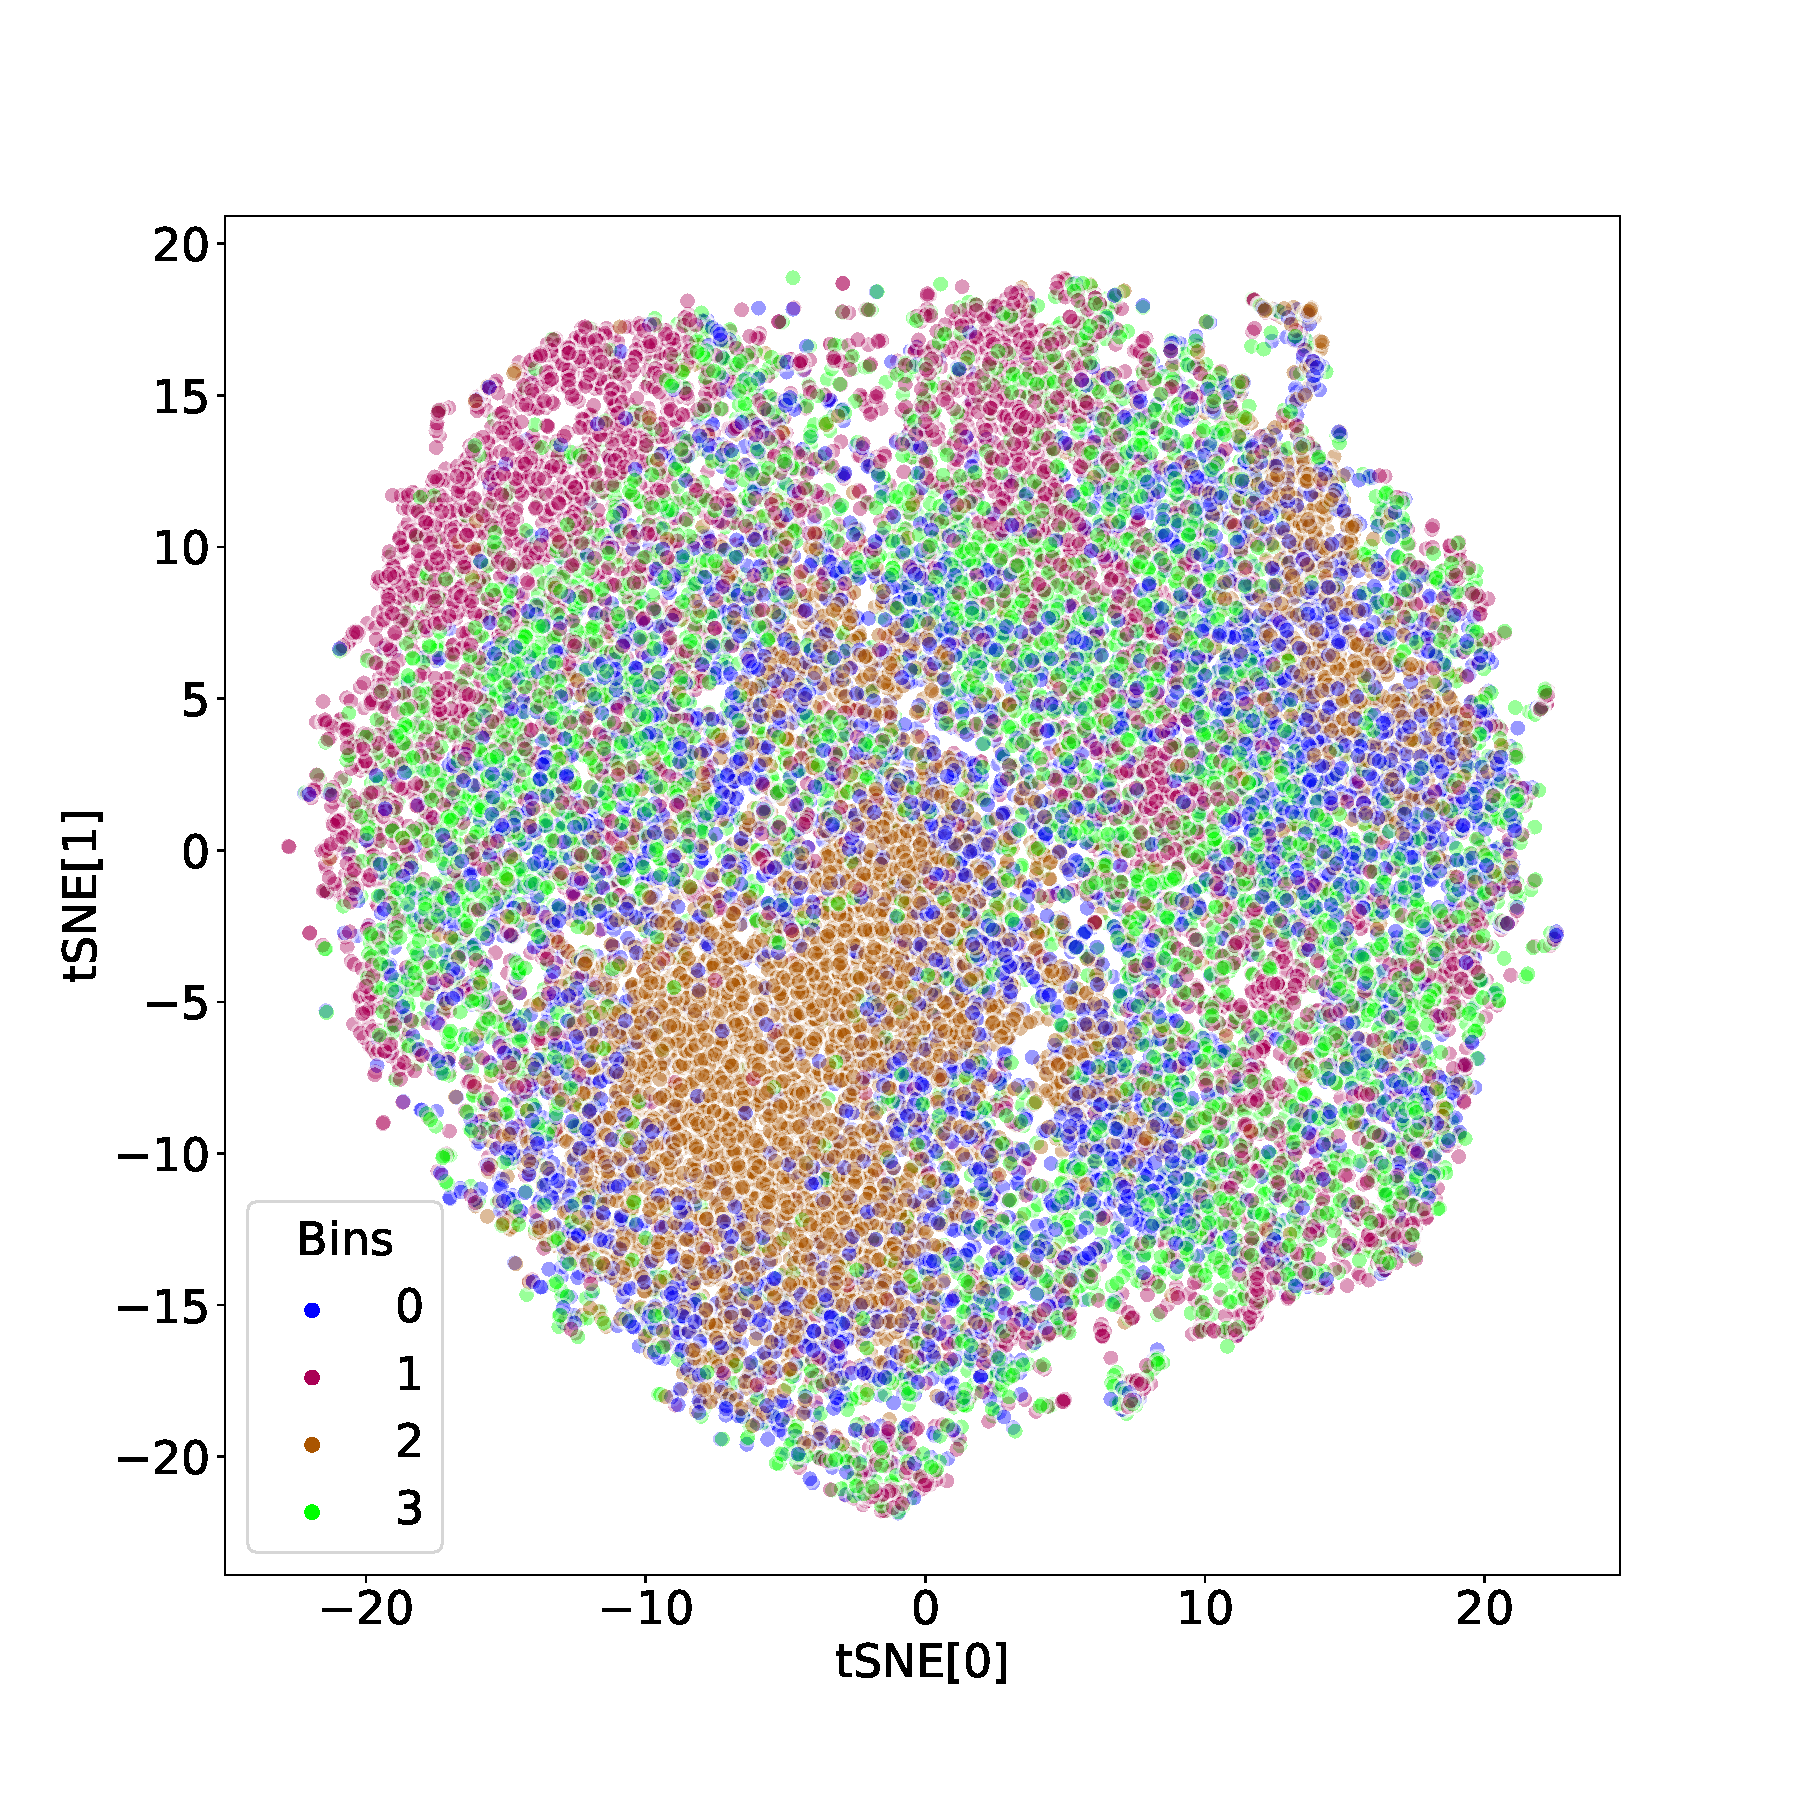
\includegraphics[width=\textwidth]{figures/iclr-age-pred-tsne.pdf}
    \label{fig-tsne-age2}
  \end{subfigure}%
  \begin{subfigure}{0.5\textwidth}
    \caption{Churn}
    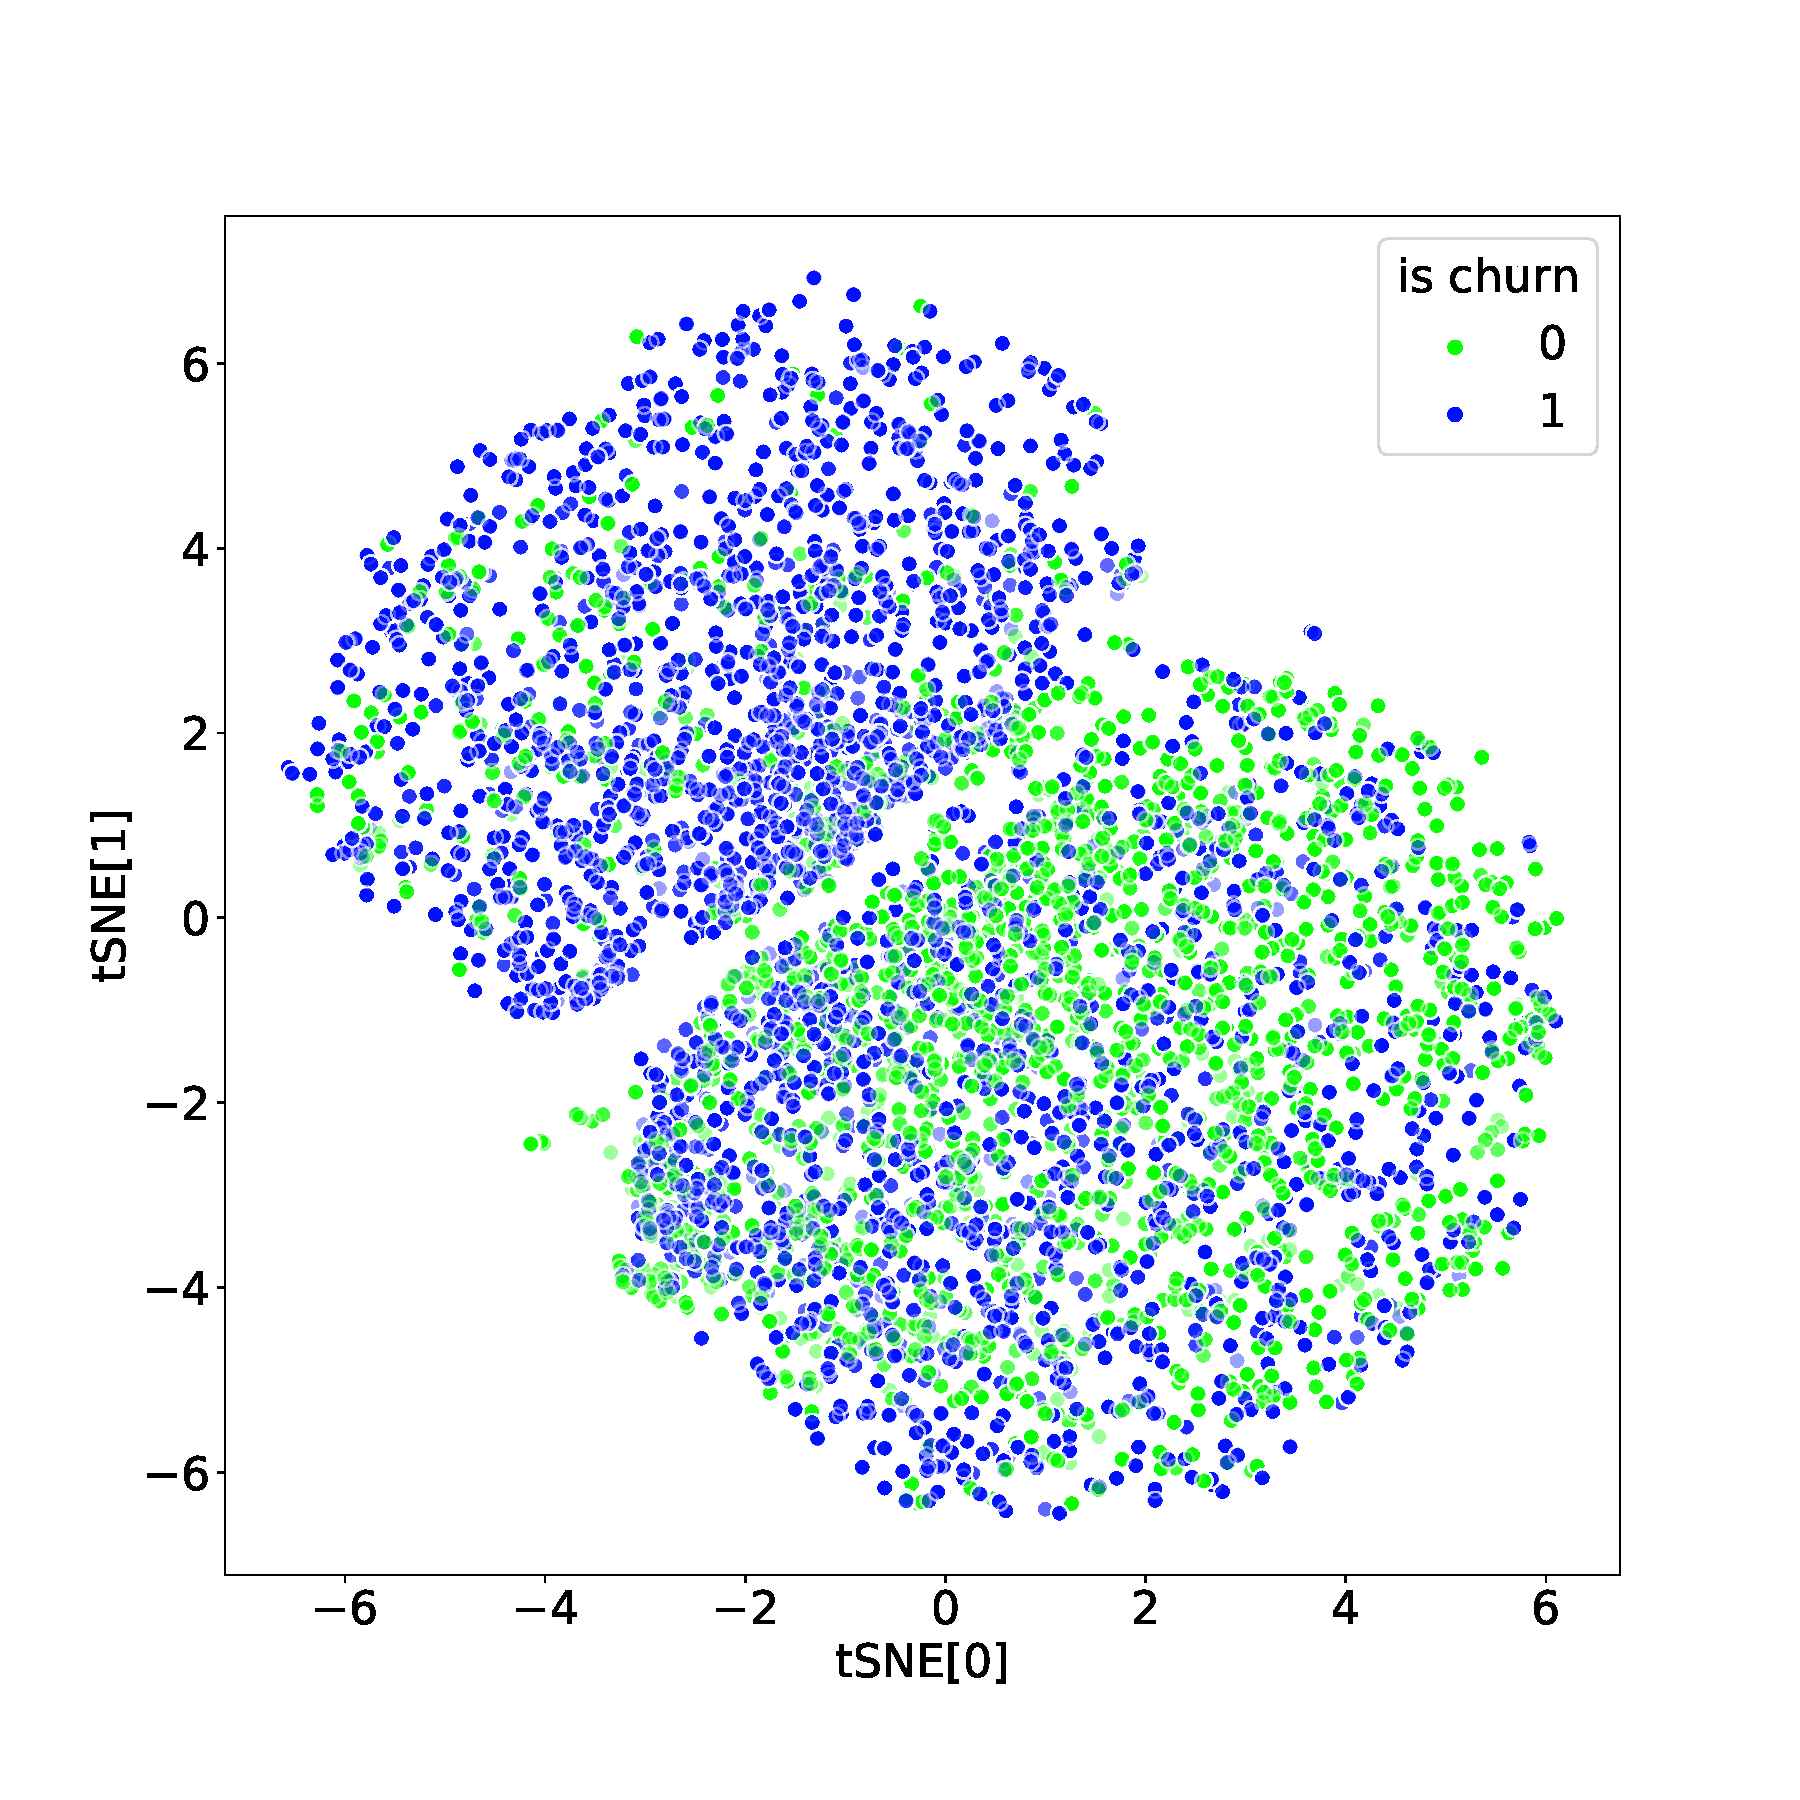
\includegraphics[width=\textwidth]{figures/iclr-churn-tsne.pdf}
    \label{fig-tsne-churn}
  \end{subfigure}
  \begin{subfigure}{0.5\textwidth}
    \caption{Assessment}
    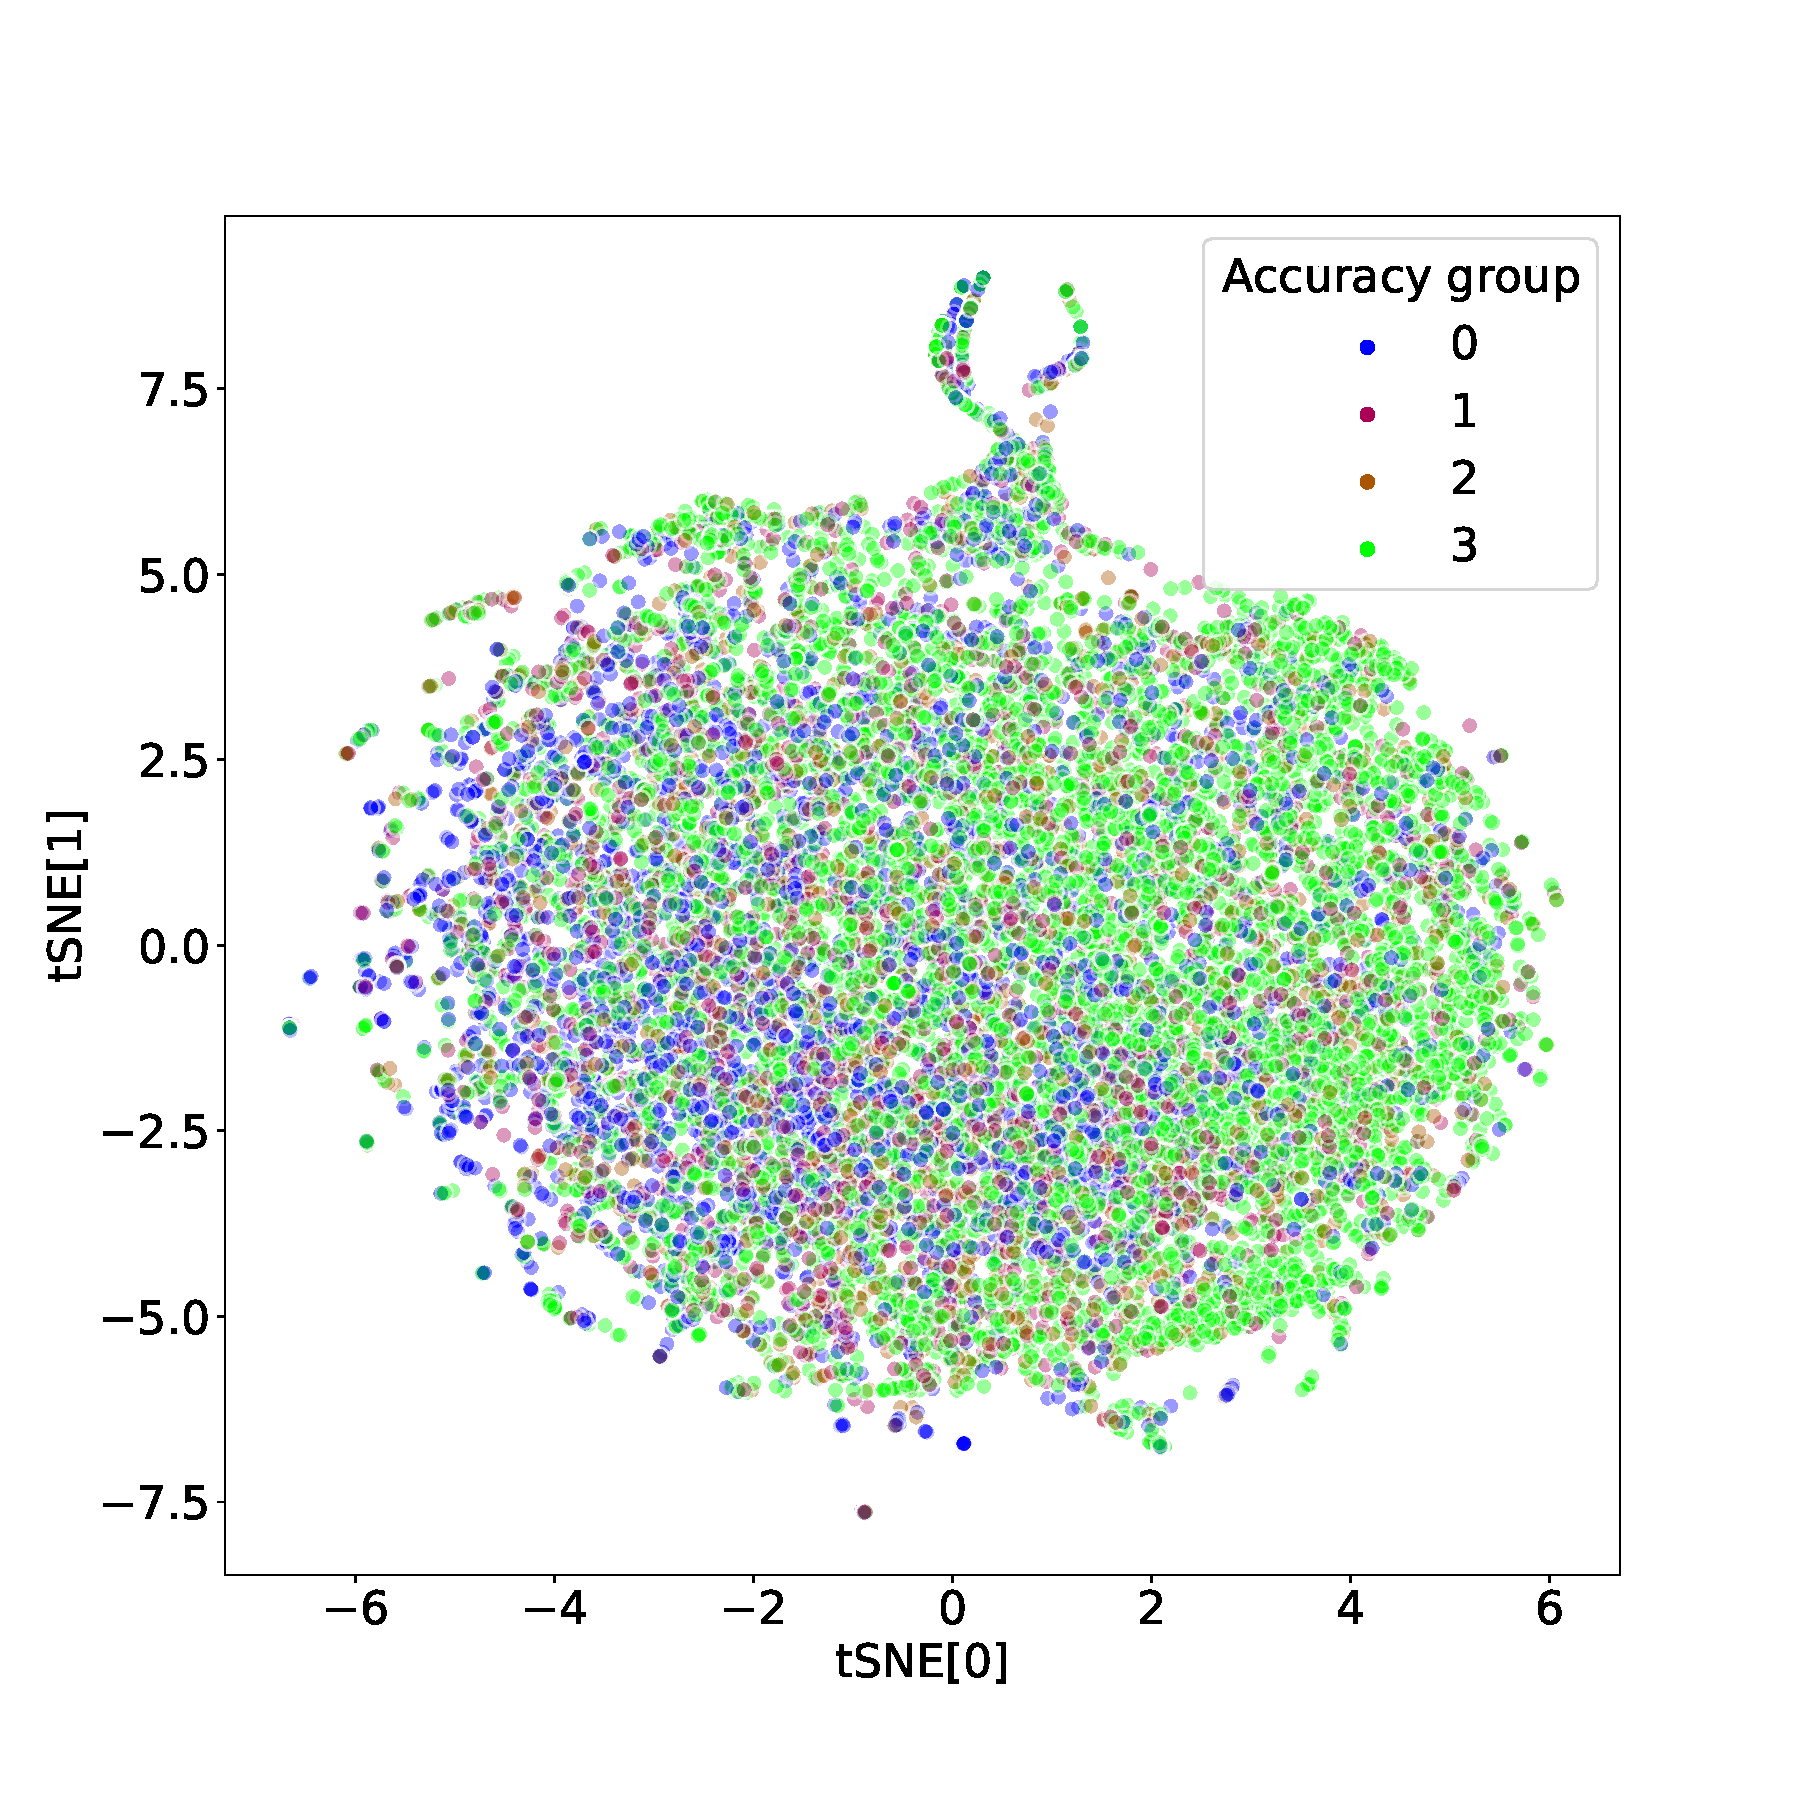
\includegraphics[width=\textwidth]{figures/iclr-bowl-tsne-accuracy_group.pdf}
    \label{fig-tsne-bowl}
  \end{subfigure}%
  \begin{subfigure}{0.5\textwidth}
    \caption{Retail}
    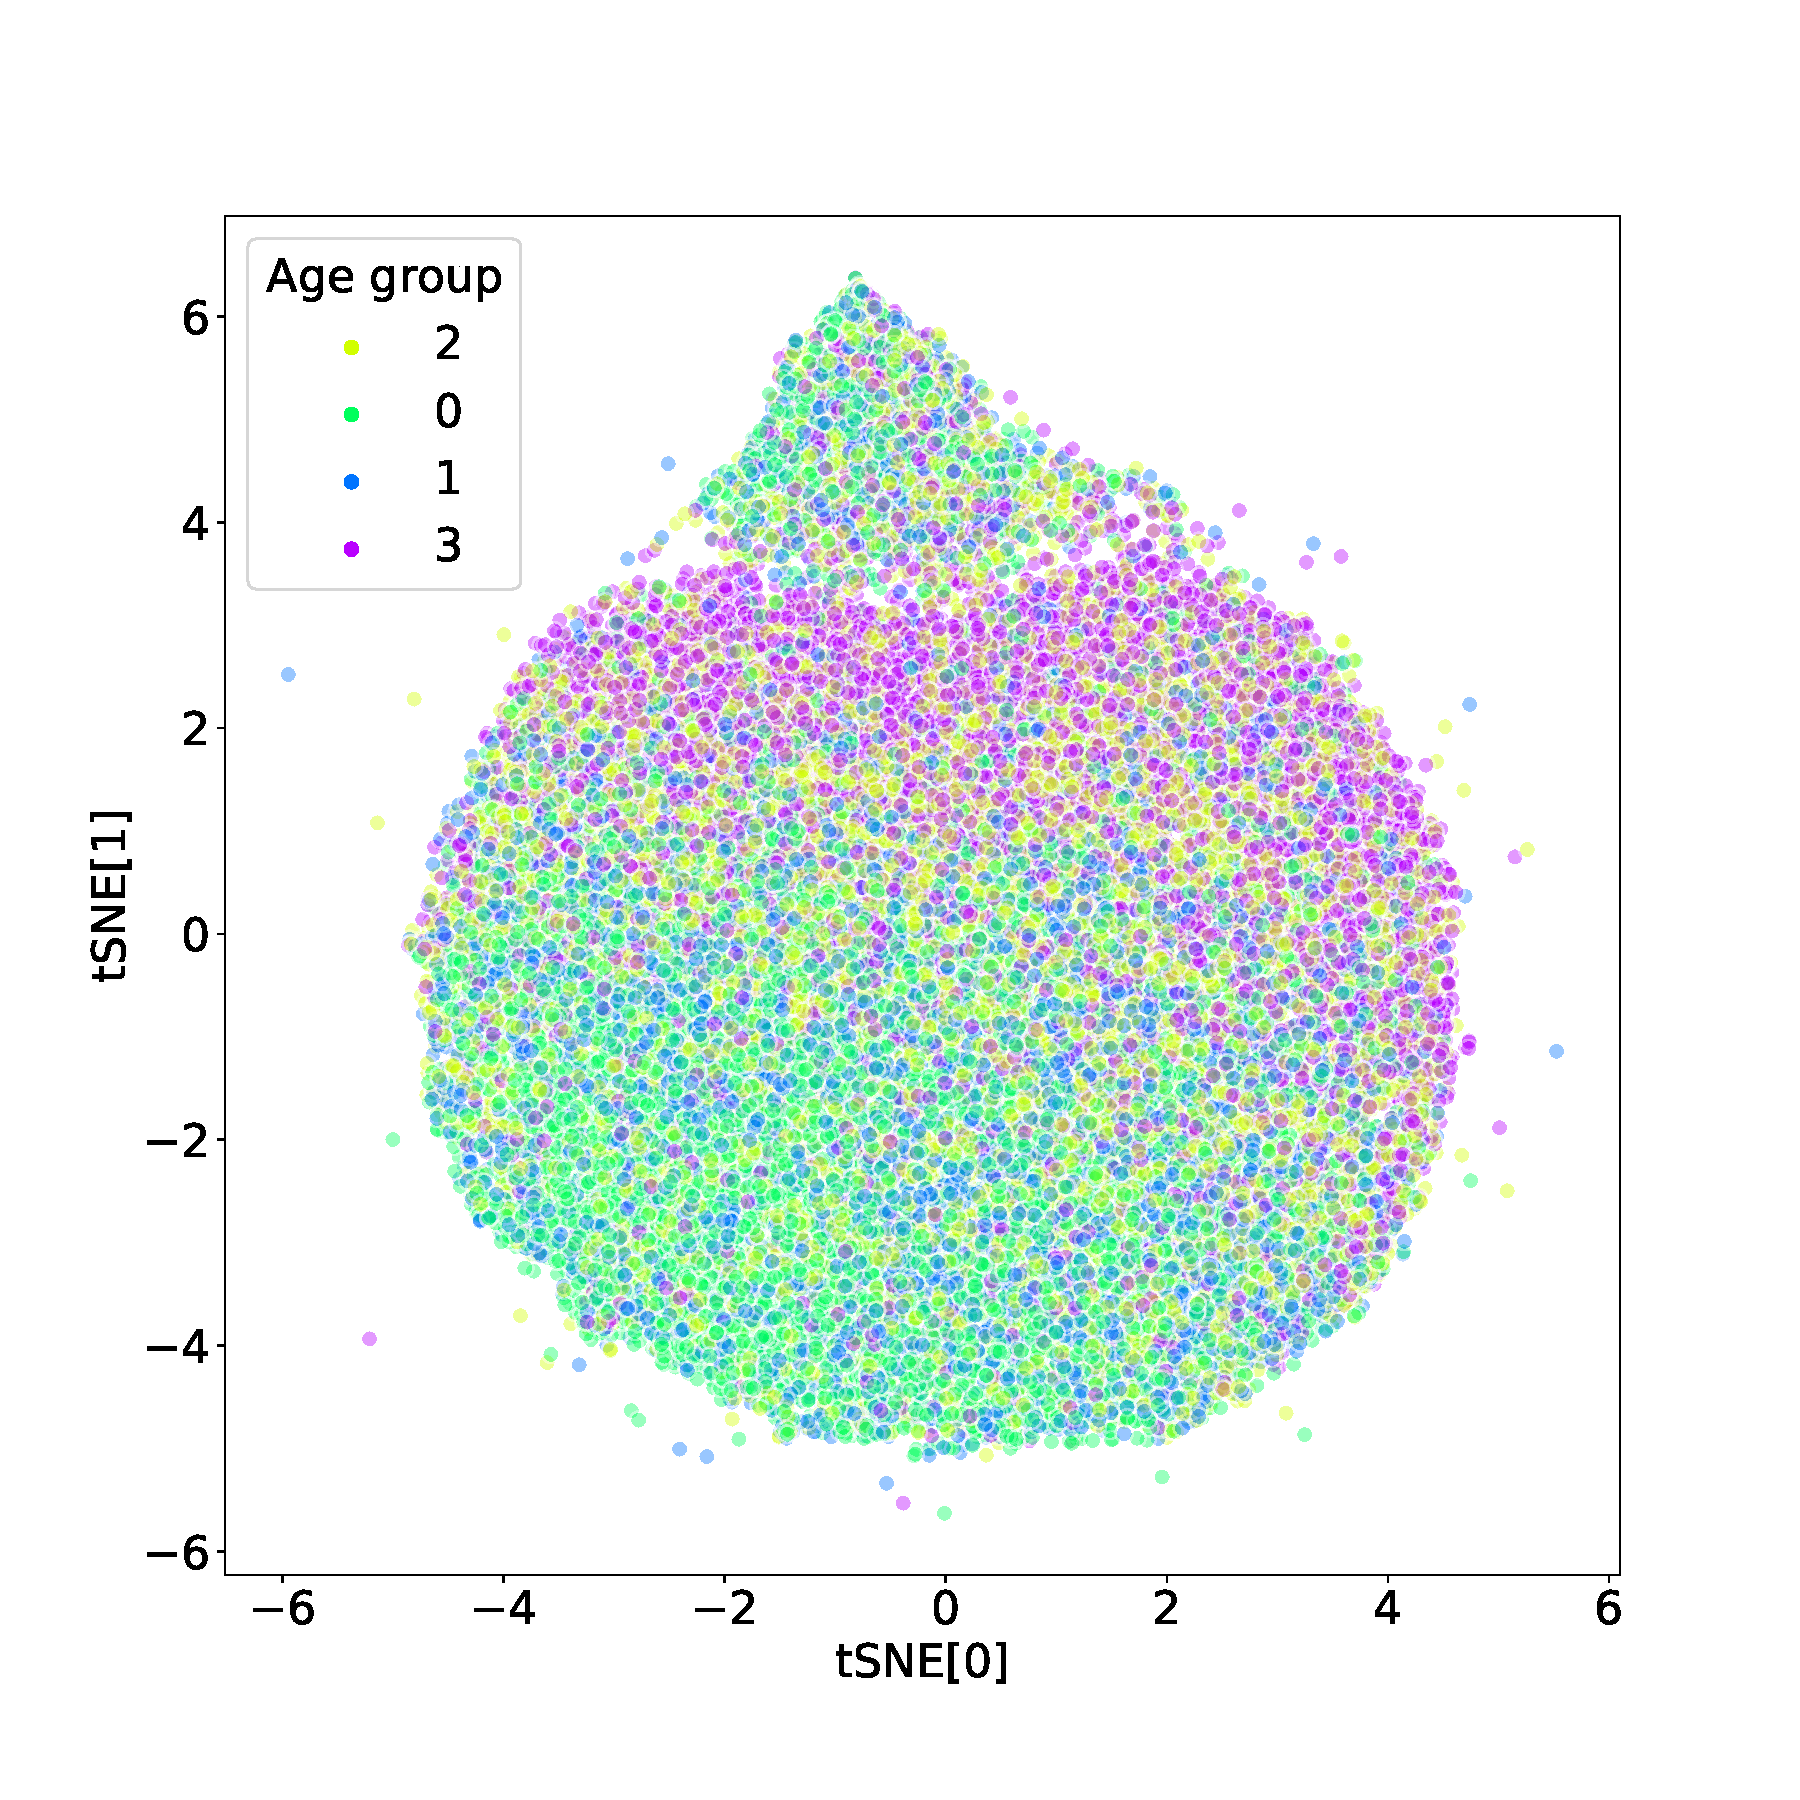
\includegraphics[width=\textwidth]{figures/iclr-x5-tsne-age_bin.pdf}
    \label{fig-tsne-x5}
  \end{subfigure}
\end{figure}

\clearpage

\end{comment}

\end{document}
